% Created 2025-07-31 Thu 17:26
% Intended LaTeX compiler: xelatex
\documentclass[a4paper,11pt]{book}
\usepackage{graphicx}
\usepackage{longtable}
\usepackage{wrapfig}
\usepackage{rotating}
\usepackage[normalem]{ulem}
\usepackage{amsmath}
\usepackage{amssymb}
\usepackage{capt-of}
\usepackage{hyperref}
\usepackage{minted}
\usepackage[paperwidth=6in,paperheight=9in,margin=1in]{geometry}
\setlength{\headheight}{25pt} % Pour éviter l'avertissement fancyhdr
\usepackage{fontspec}
\setmainfont{Palatino} % Conserver Palatino
\setsansfont{Helvetica Neue} % Ou .SF Pro Text
\setmonofont{Courier} % Une police monospace présente sur macOS
\usepackage{unicode-math}
\setmathfont{STIX Two Math} % Tentative avec STIX Two Math (plus fiable)
\usepackage{polyglossia}
\setmainlanguage{french}
\setotherlanguage{english}
\usepackage{csquotes}
\MakeAutoQuote*{«}{»} % Guillemets français automatiques
\usepackage{fancyhdr}
\pagestyle{fancy}
\fancyhf{} % Clear all headers and footers
\fancyhead[L]{\nouppercase{\leftmark}} % Chapter name on left header
\fancyhead[R]{\thepage} % Page number on right header
\fancyfoot[C]{\nouppercase{\rightmark}} % Section name on center footer
\renewcommand{\headrulewidth}{0.4pt}
\renewcommand{\footrulewidth}{0.4pt}
\fancypagestyle{plain}{\fancyhf{}\renewcommand{\headrulewidth}{0pt}\renewcommand{\footrulewidth}{0pt}} % Pour la première page de chaque chapitre
\usepackage{hyperref}
\hypersetup{
colorlinks=true,
linkcolor=orange,
citecolor=purple,
filecolor=magenta,
urlcolor=cyan,
}
\usepackage{imakeidx}
\makeindex
\usepackage[acronym, nonumberlist, toc]{glossaries}
\newglossaryentry{absorbant}{
name={élément absorbant},
description={
Un élément absorbant dépend de l'opération et de la structure
algébrique considérée. Concrètement, pour la multiplication
le nombre zéro \(0\) est un élément absorbant car tout nombre
réel \(x\in\mathbb{R}\) qui le multiplie donnera zéro
\[\forall x\in\mathbb{R},\,x\times 0 = 0 = 0\times x\]
Si on rajoute l'infini \(\infty\) alors ça devient un élément
absorbant pour l'addition. En effet,
\[\forall x\in\mathbb{R},\,x + \infty = \infty = \infty + x\]
Qu'il s'agisse de l'infini postif \(+\infty\) ou de l'infini
négatif \(-\infty\). Ces notions seront approfondies dans les
études supérieures (post bac)
}
}
\newglossaryentry{amplitude}{
name={amplitude (d'un intervalle)},
description={
L'amplitude d'un intervalle est sa longueur c'est donc
\(+\infty\) si l'une des bornes est infinie et sinon
c'est un nombre réel positif égal à la différence
entre la borne supérieure et la borne inférieure.
Concerètement si \[I = [a ; b]\] alors son amplitude vaut
\[A(I) = b - a\]
si \[I = ]-\infty ; b[\] alors son amplitude vaut
\[A(I) = b - (-\infty ) = +\infty \]
si \[I = [a ; +\infty [\] alors son amplitude vaut
\[A(I) = +\infty - a = +\infty \]
si \[I = ]-\infty ; +\infty [\] alors son amplitude vaut
\[A(I) = +\infty - (-\infty ) = +\infty \]
Le résultat est toujours positif
}
}
\newglossaryentry{float}{
name={type float},
description={
En Programmation Python le type \texttt{float} pour
l'abréviation de l'anglais \emph{floating point number}
(nombre à virgule flottante car les anglo-saxons utilisent
le point comme séparateur décimal) désigne un sous-ensemble fini
(selon la capacité de mémoire de la machine) de
l'ensemble des nombres décimaux \(\mathbb{D}\).
Par exemple le plus grand \texttt{float} en Python
vaut envrion \[1,79769313\times 10^{308}\]
et son opposé pour les négatifs.
Le zéro n'existant pas en informatique il y a une valeur
qui s'en rapproche et vaut environ
\[2.2250738585\times 10^{-308}\]
Ces nombres seront amenés à grandir à mesure que les capacités
de stockage des machines augmentent
}
}
\newglossaryentry{inf}{
name={borne inférieure},
description={
La borne inférieure d'un intervalle est \(-\infty\)
si l'intervalle est de la forme \(]-\infty ; b]\)
peu importe qu'il soit ouvert ou fermé ou que \(b\)
soit un réel ou \(+\infty\) et sinon c'est le réel \(a\).
Concerètement si \[I = [a ; b]\] alors sa borne inférieure vaut
\[\inf(I) = a\]
si \[I = ]-\infty ; b\] alors sa borne inférieure vaut
\[\inf(I) = -\infty \]
Dans ce cas on dit que l'ensemble n'est pas minoré. En effet,
il n'existe aucun nombre plus petit que l'infini négatif
\(-\infty\). Ces notions seront approfondies dans les études
supérieures (post bac)
}
}
\newglossaryentry{sup}{
name={borne supérieure},
description={
La borne supérieure d'un intervalle est \(+\infty\)
si l'intervalle est de la forme \(]a ; +\infty [\)
peu importe qu'il soit ouvert ou fermé ou que \(a\)
soit un réel ou \(-\infty\) et sinon c'est le réel \(b\).
Concerètement si \[I = [a ; b]\] alors sa borne inférieure vaut
\[\sup(I) = b\]
si \[I = [a ; +\infty [\] alors sa borne supérieure vaut
\[\sup(I) = +\infty \]
Dans ce cas on dit que l'ensemble n'est pas majoré.
En effet, il n'existe aucun nombre plus grand que l'infini
positif \(+\infty\). Ces notions seront approfondies dans
les études supérieures (post bac)
}
}
\newglossaryentry{distance}{
name={distance},
description={
La longueur entre un nombre \(x\) et zéro est sa valeur absolue.
Concrètement \(\lvert x \rvert = x\) si \(x \geq 0\) et
\(\lvert x \rvert = -x\) si \(x < 0\). Par exemple
\(d(-3, 0) = \lvert -3 \rvert = 3\) et
\(d(0, 4) = \lvert 4 \rvert = 4\)
}
}
\newglossaryentry{nb-dec}{
name={nombres décimaux},
description={
L'ensemble \(\mathbb{D}\) des nombres décimaux inclut tous les
nombres entiers (relatifs) \(\mathbb{Z}\) et tous les nombres
entiers naturels \(\mathbb{N}\). Pour la faire simple, ce sont
les nombres avec un nombre fini de chiffres après la virgule.
Par exemple : \(2 = 2,0\in\mathbb{D},\,\)
\(\dfrac{1}{2} = 0,5\in\mathbb{D}\) mais
\(\dfrac{1}{3}\not\in\mathbb{D}\) car le nombre de chiffre
après la virgule est inifini
}
}
\newglossaryentry{nb-nat}{
name={nombres entiers naturels},
description={
L'ensemble \(\mathbb{N}\) des nombres entiers naturels
est constitué des nombres qu'on peut compter avec les doigts
y compris 0 donc \[\mathbb{N} = \{0, 1, 2, 3, \dots\}\]
C'est un ensemble dénombrable infini.
Les nombres négatifs n'en font pas partie. Pour les anglo-saxons
le nombre zéro n'en fait pas partie
}
}
\newglossaryentry{nb-rel}{
name={nombres entiers relatifs},
description={
L'ensemble \(\mathbb{Z}\) des nombres entiers relatifs
est constitué de tous les nombres entiers naturels
\(\mathbb{N}\) ainsi que leurs opposés donc
\[\mathbb{Z} = \{\dots , -3, -2, -1, 0, 1, 2, 3, \dots\}\]
En anglais, en Python et dans les langages de programmation
on les appelle \emph{integer} (\texttt{int} en Python)
}
}
\newglossaryentry{nb-ratio}{
name={nombres rationnels},
description={
L'ensemble \(\mathbb{Q}\) des nombres rationnells inclut tous les
nombres décimaux \(\mathbb{D}\),
entiers relatifs \(\mathbb{Z}\),
entiers naturels \(\mathbb{N}\) et toutes les fractions
dont le numérateur est un nombre entier relatif et le
dénominateur un entier naturel strictement positif.
Par exemple \(\dfrac{1}{3}\in\mathbb{Q}\)
}
}
\newglossaryentry{nb-reels}{
name={nombres réels},
description={
L'ensemble \(\mathbb{R}\) des nombres réels inclut tous les
nombres rationnels \(\mathbb{Q}\) et irrationnels (comme \(\pi\),
le nombre d'or \(\Phi = \dfrac{1 + \sqrt{5}}{2}, \dots\)).
On peut les représenter géométriquement à l'aide d'une droite
graduée de \(-\infty\) jusqu'à \(+\infty\) sans coupure (entre
deux nombres rationnels il y a une infinité indénombrables
de réels). Ces notions de dénombrabilité et indénombrabilité
renvoient à la classification des infinis qui sera abordée
dans les études supérieures (post bac)
}
}
\newglossaryentry{nb-irr}{
name={nombres irrationnels},
description={
L'ensemble des nombres irrationnels inclut tous les réels
qui ne sont pas des nombres rationnels \(\mathbb{Q}\) (comme \(\pi\),
le nombre d'or \(\Phi = \dfrac{1 + \sqrt{5}}{2},\,\)
\(\sqrt{2}\dots\)).
Il en existe une infinité
}
}
\newglossaryentry{nb-prem}{
name={nombre premier},
description={
Un nombre entier naturel est dit premier s'il n'admet que
\(1\) et lui-même comme diviseurs positifs. Par exemple les
nombres \(2, 3, 5, 7, 11,\dots\) sont premiers mais
\(4 = 2\times 2\) n'est pas premier.
Il en existe une infinité. Leur particularité est qu'il est
très difficile de déterminer si un (très grand) nombre est
premier ou non. C'est précisément sur cette difficulté que
repose toute l'industrie de la sécurité bancaire, Bitcoin et le
chiffrement en général. Ils sont donc très utile dans la vie réelle
}
}
\newglossaryentry{inclus}{
name={inclusion ensembliste},
description={
On dit qu'un ensemble A est inclus dans un autre ensemble B
si tous les éléments de A sont aussi dans B. Par exemple
l'intervalle \[I_0 = [0 ; 1]\] est inclus dans l'intervalle
\[I_1 = [-1 ; 2]\] on note \[I_0\subset I_1\]
En effet si \(0\leq x\leq 1\) alors
\(-1\leq x\leq 2\). Par contre \(1,5\in I_1\)
mais \(1,5\not\in I_0\). Certains ensembles ne sont
pas comparables, par exemple l'intervalle \[I_2 = [4 ; 5]\]
n'est ni dans \(I_0\) ni dans \(I_1\) mais il ne contient
aucun des deux non plus. La France ne contient pas l'Angleterre
et réciproquement
}
}
\newglossaryentry{int}{
name={type int},
description={
En Programmation Python le type \texttt{int} pour
l'anglais \emph{integer} est un sous-ensemble fini
(selon la capacité de mémoire de la machine) de
l'ensemble des entiers relatifs \(\mathbb{Z}\).
Par exemple en utilisant le module \texttt{numpy}
les \texttt{numpy.int32} (entiers codés sur 32 bits)
varient entre \(-2^{31}\) et \(2^{31} - 1\).
Pour donner un ordre de grandeur grossier \(2^{10} \simeq 10^3\).
Donc donc on est sur l'ordre de 2 milliards pour \(2^{31}\).
Il existe des types d'entiers codés sur 64 bits et ainsi de suite
}
}
\newglossaryentry{intervalle}{
name={intervalle},
description={
Un intervalle est un ensemble infini de nombres
compris entre une borne inférieure (éventuellement
\(-\infty\)) et une borne supérieure (éventuellement
\(+\infty\)).
Concerètement on a 8 types d'intervalles
\[I_1 = ]-\infty ; b[\]
\(I_1\) est ouvert, non borné à gauche et borné à droite.
Géométriquement il s'agit d'une demi-droite privée de son point
d'origine à droite.
\[ -\infty ---- x ---- b [----> +\infty \]
\[I_2 = ]-\infty ; b]\]
\(I_2\) est fermé, non borné à gauche et borné à droite.
Géométriquement il s'agit d'une demi-droite contenant son point
d'origine à droite.
\[ -\infty ---- x ---- b] ----> +\infty \]
\[I_3 = ]a ; b[\]
\(I_3\) est ouvert et borné.
Géométriquement il s'agit d'un segment privé de ses deux extrémités.
\[ -\infty ----] a ---- x ---- b [----> +\infty \]
\[I_4 = ]a ; b]\]
\(I_4\) est borné, ouvert à gauche et fermé à droite.
Géométriquement il s'agit d'un segment privé de son extrémité gauche.
\[ -\infty ----] a ---- x ---- b] ----> +\infty \]
\[I_5 = [a ; b[\]
\(I_5\) est borné, fermé à gauche et ouvert à droite.
Géométriquement il s'agit d'un segment privé de son extrémité droite.
\[ -\infty ---- [a ---- x ---- b [----> +\infty \]
\[I_6 = [a ; +\infty [\]
\(I_6\) est fermé, borné à gauche et non borné à droite.
Géométriquement il s'agit d'une demi-droite contenant de son point
d'origine à gauche.
\[ -\infty ---- [a ---- x ----> +\infty \]
\[I_7 = ]a ; +\infty [\]
\(I_7\) est ouvert, borné à gauche et non borné à droite.
Géométriquement il s'agit d'une demi-droite privée de son point
d'origine à gauche.
\[ -\infty ----] a ---- x ----> +\infty \]
\[I_8 = ]-\infty ; +\infty [\]
\(I_8 = \mathbb{R}\) est ouvert ET fermé  et non borné.
Géométriquement il s'agit d'une droite.
\[ -\infty ----] a ---- x ----> +\infty \]
Une droite n'a ni extrémité à gauche ni à droite, c'est un ensemble
infini tout comme l'ensemble des réels \(\mathbb{R}\)
}
}
\newglossaryentry{part-dec}{
name={partie décimale},
description={
Pour tout nombre réel \(x\) les nombres après la virgule
constituent ce qu'on appelle la partie décimale.
Par exemple le nombre décimal
\[\dfrac{9}{8} = 1,125 = 1 + \dfrac{1}{8}\]
a pour partie décimale
\[\left\{\dfrac{9}{8}\right\} = 0,125 = \dfrac{1}{8}\]
Les nombres entiers ont une partie décimale nulle.
Par exemple le nombre entier 3 a pour partie décimale 0
}
}
\newglossaryentry{part-ent}{
name={partie entière},
description={
Pour tout nombre réel \(x\) le nombre avant la virgule
constitue ce qu'on appelle la partie entière.
Par exemple le nombre décimal
\[\dfrac{9}{8} = 1,125 = 1 + \dfrac{1}{8}\]
a pour partie entière
\[\left\lfloor\dfrac{9}{8}\right\rfloor = 1 = \dfrac{8}{8}\]
Les nombres entiers sont égaux à leur partie entière.
Par exemple le nombre entier 3 a pour partie entière lui-même
c'est-à-dire 3
}
}
\newglossaryentry{part-frac}{
name={partie fractionnaire},
description={
La partie fractionnaire est juste un autre nom pour la partie
décimale. C'est rigoureusement la même chose
}
}
\newglossaryentry{rab}{
name={raisonnement par l'absurde},
description={
Le raisonnement par l'absurde consiste à supposer le contraire
de ce qu'on veut montrer puis à chercher à enchaîner des
déductions logiquement valide jusqu'à aboutir à une contradiction
absurde avec l'hypothèse de départ. De cette manière, si le
contraire de ce qu'on veut montrer est faux alors ce qu'on veut
montrer est vrai. Ce raisonnement s'appuie sur le principe du
tiers exclu. Par conséquent il existe des situations et des
systèmes logiques qui refusent ce type de raisonnement
}
}
\newglossaryentry{rac}{
name={raisonnement par contraposition},
description={
Le raisonnement par contraposition se base sur l'équivalence
logique entre une implication P = << A implique B >>
\[P = (A\Rightarrow B)\)\]
et sa contraposée Q = << non(B) implique non(A) >>
\[Q = (\neg B\Rightarrow \neg A)\)\]
Par exemple si A = << Le nombre \(n\) est impair >>
et B = << Le nombre \(n^2\) est impair >>
il est facile de montrer que
\[P = (A\Rightarrow B)\)\]
est vraie, en effet, le carré d'un nombre impair est aussi impair.
En revanche sa contraposée est impossible à démontrer
de manière directe. Mais grâce à l'équivalence logique, montrer
P revient à montrer Q. Pour prouver qu'il y a équivalence logique
on peut utiliser une table de vérité. Cela sera abordé dans
les études supérieures (post bac)
}
}
\newglossaryentry{tiers-exclu}{
name={principe du tiers exclu},
description={
Le principe du tiers exclu consiste à dire que dans un système
de logique classique toute affirmation est soit vraie, soit
fausse. Par exemple pour tout nombre réel \(x\) soit l'affirmation
\[P = (x \geq 2)\]
est vraie soit c'est son contraire
\[Q = \neg P = (x < 2)\]
Cela paraît évident mais il existe de nombreuses situations pour
lesquelles ce principe est faux. Par exemple si on considère
la proposition P = << Cette tasse est chaude. >> Dans cette
situation la logique classique serait inefficace alors on utiliserait
plutôt la logique floue qui nous permettrait de dire par exemple
l'affirmation P a une valeur de 70\%. Cet exemple de la vie
courante sert uniquement à vous rappeler qu'en science on utilise
différents modèles selon le contexte du problème à résoudre
}
}
\newacronym{pgcd}{PGCD}{Plus Grand Commun Diviseur}
\AtBeginDocument{\input{glossaire.tex}}
\makeglossaries % Doit être appelé après toutes les définitions \newglossaryentry
\usepackage{graphicx} % Pour inclure des images
\graphicspath{{./img/}} % Définit le chemin par défaut pour les images
\usepackage{enumitem} % Pour personnaliser les listes
\usepackage{caption} % Pour personnaliser les légendes
\usepackage{subcaption} % Pour les sous-figures
\usepackage{tikz} % Pour les graphiques vectoriels
\usepackage{pgfplots} % Pour les tracés de fonctions
\pgfplotsset{compat=1.18}
\usepackage{xcolor} % Pour les couleurs
\definecolor{MyOrange}{HTML}{FF6600}
\usepackage{minted}
\usepackage{environ} % Pour créer de nouveaux environnements
\usepackage{tocloft}
\renewcommand{\cftsecleader}{\cftdotfill{\cftdotsep}}
\renewcommand{\cftsecfont}{\color{orange}\bfseries}
\usepackage[most]{tcolorbox}
\newtcolorbox{myquote}[1]{%
colback=blue!3!white,%
colframe=blue!75!black,%
fonttitle=\bfseries\itshape\Large\sffamily,%
fontupper=\itshape\large\rmfamily,%
sharp corners,%
boxrule=1pt,%
left=6mm, right=6mm, top=6mm, bottom=6mm,%
title=#1%
}
\author{Laurent Garnier}
\date{\today}
\title{Manipuler les nombres réels}
\hypersetup{
 pdfauthor={Laurent Garnier},
 pdftitle={Manipuler les nombres réels},
 pdfkeywords={mathématiques, exercices, calcul, géométrie, éducation, lycée},
 pdfsubject={Ce livre propose des exercices et explications pour manipuler les nombres réels},
 pdfcreator={Emacs 29.4 (Org mode 9.6.15)}, 
 pdflang={Fr}}
\begin{document}

\maketitle
\tableofcontents

\setcounter{tocdepth}{1}
\tableofcontents







\part{À qui s'adresse ce livre}
\label{sec:orge56b974}
\label{org8cd9742}
\label{page:sec1intro}



\begin{myquote}{Josiah Willard Gibbs}
\enquote{Mathematics is a language.}\footnote{Voir la page Wikipédia sur Gibbs : \url{https://en.wikipedia.org/wiki/Josiah_Willard_Gibbs  }}
\end{myquote}
\index{Gibbs, Josiah Willard}
\clearpage

Ce livre s'adresse initialement aux élèves de seconde du système
scolaire français. Mais il sera probablement très utile à un élève
de fin de collège qui voudrait assurer son entrée au lycée. Il sera
également très utile à un élève de première qui voudrait s'assurer
qu'il maîtrise bien les notions de la classe de seconde. Enfin un
quatrième public qui pourrait directement être visé est celui des
enseignants, profs particuliers ou encore tuteurs (professionnels ou
amateurs) qui souhaiteraient consulter des ressources utiles et
utilisables pour aider les lycéens.

De façon plus générale, même si je reprends exactement la structure
du \href{https://eduscol.education.fr/document/24553/download}{programme officiel} que vous pouvez consulter ici :
\url{https://eduscol.education.fr/document/24553/download}, il me semble
que ce livre pourrait être utile à quiconque souhaite approcher les
mathématiques de façon honnête, rigoureuse et avec un soucis de
compréhension. Tout en respectant le niveau du programme, j'essaierai
dès que possible de prolonger la perspective.

Vous pouvez d'ores et déjà mettre en pratique de façon interactive
toutes les notions abordées grâce aux codes Python accessibles sur
Google Colab à l'adresse communiquée dans la section concernée
lorsque vous aurez rempli ce petit formulaire :
\url{https://forms.gle/qY8ym3ZxSo9NVH3S7} (vous trouverez également les
corrections de tous les exercices du livre).

Si vous constatez une erreur que ça soit une erreur de calcul, une
faute de frappe ou quoique ce soit merci de me contacter à l'adresse
indiquée dans le formulaire afin de me la signaler et que je puisse
la corriger. Idem si vous avez des suggestions d'amélioration.

Bonne lecture.
\clearpage

\part{Contenus}
\label{sec:orge938bac}
\label{org4fcdbf1}
\label{page:sec2contents}

\begin{myquote}{Marc du Sautoy}
\enquote{Mathematics has beauty and romance. It’s not a boring place to be,
the mathematical world. It’s an extraordinary place; it’s worth
spending time there.}\footnote{Voir la page Wikipédia sur Marcus du Sautoy : \url{https://en.wikipedia.org/wiki/Marcus_du_Sautoy}}
\end{myquote}
\index{du Sautoy, Marc}
\clearpage

\label{org2ce8f1f}
\label{page:content-menu}
\begin{itemize}
\item \hyperref[orge386a9d]{Contenu 1 : Nombres réels, droite numérique}
page~\pageref{page:sec2.1content1}
\item \hyperref[org31d1c9a]{Contenu 2 : Intervalles de nombres réels}
page~\pageref{page:sec2.2content2}
\item \hyperref[org0ecf993]{Contenu 3 : Distances}
page~\pageref{page:sec2.3content3}
\item \hyperref[orgbdb89e7]{Contenu 4 : Disques sur la droite réelle}
page~\pageref{page:sec2.4content4}
\item \hyperref[org86f143d]{Contenu 5 : Nombres décimaux}
page~\pageref{page:sec2.5content5}
\item \hyperref[orgee452f1]{Contenu 6 : Nombres rationnels}
page~\pageref{page:sec2.6content6}
\item \hyperref[org9c65356]{Capacités attendues}
page~\pageref{page:sec3capacities}
\end{itemize}

\clearpage

\chapter{Contenu 1 : Nombres réels, droite numérique}
\label{sec:org79fe394}
\label{orge386a9d}
\label{page:sec2.1content1}
\begin{myquote}{Pythagore}
\enquote{Tout l'univers repose sur l'ensemble des entiers naturels.}\footnote{Voir la page Wikipédia sur Pythagore : \url{https://fr.wikipedia.org/wiki/Pythagore}}
\end{myquote}
\index{Pythagore}

\clearpage


Cette partie développe la rubrique intitulée :

<< Ensemble \(\mathbb{R}\) des nombres réels, droite numérique >>

dans le \href{https://eduscol.education.fr/document/24553/download}{programme officiel}\footnote{Voir le site officiel du programme de mathématiques
en classe de seconde dans le système scolaire français :
\url{https://eduscol.education.fr/document/24553/download}}.
\clearpage

\label{orga5086f2}
\label{page:content1-menu}
\begin{itemize}
\item \hyperref[orgfb34aa0]{Savez-vous compter sur vos doigts ?}
page~\pageref{page:sec2.1.1digits}
\item \hyperref[orgdf90d81]{Tout est relatif}
page~\pageref{page:sec2.1.2int}
\item \hyperref[org1213e07]{Les ordinateurs s'en contentent}
page~\pageref{page:sec2.1.3cpu}
\item \hyperref[orgeac9191]{Êtes-vous rationnels ?}
page~\pageref{page:sec2.1.4rational}
\item \hyperref[orgff5d9b3]{Au-delà du réel}
page~\pageref{page:sec2.1.5real}
\item \hyperref[org084e38f]{Raisonnement par contraposition}
page~\pageref{page:sec2.1.6cp}
\item \hyperref[orgfd91183]{Exercice 1}
page~\pageref{page:sec2.1.7exo1}
\item \hyperref[orgce66a51]{Exercice 2 : Python}
page~\pageref{page:sec2.1.8exo2}
\item \hyperref[org2ce8f1f]{Menu précédent}
page~\pageref{page:content-menu}
\item \hyperref[org31d1c9a]{Contenu suivant}
page~\pageref{page:sec2.2content2}
\end{itemize}

\clearpage

\section{Savez-vous compter sur vos doigts ?}
\label{sec:org255b4f7}
\label{orgfb34aa0}
\label{page:sec2.1.1digits}
Savez-vous résoudre l'équation \(x - 1 = 0\) ? Je vous laisse
réfléchir et je vous donnerai la solution plus tard.

Imaginez que vous êtes en train de jouer à votre jeu vidéo
préféré. Il vous reste 3 points de vie, combien pouvez-vous en
perdre avant de mourir (dans le jeu) ? Idem, je vous laisse
réfléchir.

En général, lorsque vous entrez en seconde vous êtes âgé de 15 ans,
du coup combien d'années vous séparent de votre majorité ?

Ces trois questions traitent du même genre de problèmes, la
résolution des équations algébriques du premier degré impliquant
les nombres les plus simples que vous connaissez à savoir les
\gls{nb-nat}\index{nombres!entiers naturels}. Pour la
faire simple il s'agit des nombres utiles pour compter le nombre de
doigts que vous possédez, le nombre d'enfants dans une famille et
toutes les choses qu'on peut dénombrer de zéro à l'infini\index{infini}.

On note :
\[\mathbb{N} = \{0, 1, 2, 3,\dots\}\]
l'ensemble des entiers naturels\index{ensemble!des entiers naturels}.

\begin{itemize}
\item Équation 1 : \(x - 1 = 0\Rightarrow x = 1\in\mathbb{N}\)
\item Équation 2 : \(3 - x = 0\Rightarrow x = 3\in\mathbb{N}\)
\item Équation 3 : \(15 + x = 18\Rightarrow x = 3\in\mathbb{N}\)
\end{itemize}


\begin{itemize}
\item \hyperref[orga5086f2]{Voir menu précédent} 
page~\pageref{page:content1-menu}
\end{itemize}

\clearpage

\section{Tout est relatif}
\label{sec:org2a76b92}
\label{orgdf90d81}
\label{page:sec2.1.2int}

Mais ces nombres sont insuffisants pour exprimer des températures
par exemple dans une ville d'Europe du Nord comme Saint Pétersbourg
en Russie ou Oslo en Norvège. En fait, même en France
métropolitaine si vous allez en Savoie vous observerez des
températures négatives en hiver et positives en été. Le signe de ces
températures est \emph{relatif} à la position du zéro.

Les \gls{nb-rel}\index{nombres!entiers relatifs} sont
constitués des nombres entiers naturels\index{entiers naturels} (les
nombres positifs qu'on a vu \hyperref[orgfb34aa0]{précédemment}\footnote{Voir page \pageref{page:sec2.1.1digits}}) auxquels on
ajoute leurs symétriques par rapport à zéro.

On les note :
\[\mathbb{Z} = \{\dots, -2, -1, 0, 1, 2, \dots\}\]

Le symbole \(\mathbb{Z}\) pour les entiers relatifs vient du mot
allemand << \emph{Zahlen} >>, qui veut dire << nombres >>.

Dans la pratique on dira simplement << les entiers >> pour désignaient
les entiers relatifs.

Ce sont également ces nombres qu'on utilise dans un ascenseur pour
indiquer si on va au sous-sol (nombre négatif) ou aux étages
supérieurs (nombres positifs).

Dans le langage de programmation Python les nombres entiers
relatifs sont représentés par le type \texttt{int} pour
\emph{integer} (qui veut dire entier relatif en anglais). Donc en Python le
\gls{int}\index{int} correspond à un nombre fini d'entiers
relatifs. 

\begin{itemize}
\item \hyperref[orgfb34aa0]{Voir section précédente}
page~\pageref{page:sec2.1.1digits}
\item \hyperref[orga5086f2]{Voir menu précédent}
page~\pageref{page:content1-menu}
\end{itemize}

\clearpage

\section{Les ordinateurs s'en contentent}
\label{sec:org22bc18d}
\label{org1213e07}
\label{page:sec2.1.3cpu}

Mais ces nombres sont encore en nombre insuffisants pour exprimer,
par exemple, les unités monétaires. Quand vous achetez une baguette,
du carburant, des fournitures scolaires ou quoique ce soit ; la
plupart du temps vous utilisez des nombres à virgules qu'on appelle
les \gls{nb-dec}\index{décimaux}.

Contrairement aux deux ensembles précédents, l'ensemble des nombres
décimaux ne peut pas être représenté de façon explicite avec des
points de suspension, il doit être définit en \emph{compréhension}. Définir
un ensemble en compréhension signifie que vous devez expliquer la
règle de construction.

On note :
\[\mathbb{D} = \left\{ \dfrac{a}{10^n}\,|\,(a, n)\in\mathbb{Z}^2\right\}\]
l'ensemble des nombres décimaux avec :
\begin{itemize}
\item le symbole <<  \(|\)  >> qui se lit <<  \emph{tel(s) que}  >>
\item et le symbole <<  \(\in\)  >> qui se lit << \emph{appartient à} >>
\end{itemize}

Commençons par la fin <<  \((a, n)\in\mathbb{Z}^2\)  >> signifie que \(a\) et
\(n\) sont tous les deux des entiers relatifs\index{entiers relatifs}. Ainsi, les décimaux\index{décimaux} sont les nombres
fractionnaires dont le numérateur est un entier relatif et le
dénominateur une puissance de 10.

Donnons quelques exemples :
\begin{itemize}
\item Exemple 1 : \[(a, n) = (1, 2)\Rightarrow d_1 = \dfrac{1}{10^2} = 0,01\]
\item Exemple 2 : \[(a, n) = (3, 4)\Rightarrow d_2 = \dfrac{3}{10^4} = 0,0003\]
\item Exemple 3 : \[(a, n) = (2, -1)\Rightarrow d_3 = \dfrac{2}{10^{-1}} = 20\]
\item Exemple 4 : \[(a, n) = (3, 0)\Rightarrow d_4 = \dfrac{3}{10^0} = 3\]
\item Exemple 5 : \[(a, n) = (-1, 2)\Rightarrow d_5 = \dfrac{-1}{10^2} = -0,01\]
\end{itemize}

Dans la programmation Python on parle du type \texttt{float}, pour
\emph{floating point number} ou nombre à virgule flottante en bon
français (puisque les anglo-saxons utilisent un point comme
séparateur décimal\index{décimal}). Concrètement le 
\gls{float}\index{float} correspond à un nombre fini de décimaux.


En prenant \(n = 0\) on obtient tous les entiers
relatifs\index{entiers relatifs}. Mais ce n'est pas suffisant pour
décrire le réel (en théorie, parce qu'en pratique les ordinateurs s'en
contentent).



\begin{itemize}
\item \hyperref[orga5086f2]{Voir menu précédent} page \pageref{page:content1-menu}
\item \hyperref[orgdf90d81]{Voir section précédente} page \pageref{page:sec2.1.2int}
\end{itemize}

\clearpage

\section{Êtes-vous rationnels ?}
\label{sec:org5825362}
\label{orgeac9191}
\label{page:sec2.1.4rational}

Imaginez que vous avez un budget pour une semaine et que vous
souhaitiez allouer une part équitable pour chaque jour. Et bien
sachez que le nombre \(\dfrac{1}{7}\) n'est pas un
décimal\index{décimal}, pas plus que le nombre \(\dfrac{1}{6}\). En
effet si vous posez la division ou que vous utilisez une machine
(calculatrice, ordinateur, tablette ou téléphone peu importe) vous
verrez que \(\dfrac{1}{7} \simeq 0,142857\dots\) et que cette séquence
\(142857\dots\) se répètent à l'infini. De même, de façon plus simple,
si vous prenez \(\dfrac{1}{6} \simeq 0,16\dots\) les 6 se répètent à
l'infini.



Posons \(x = 0,16\dots 6\dots\) où les 6 se répètent à
l'infini.

Multiplions \(x\) par 100 ainsi on obtient \(100x = 16,6\dots
6\dots\).

Multiplions \(x\) par 10 ainsi on obtient \(10x = 1,6\dots 6\dots\).

Faisons maintenant la soustraction qui va faire disparaître les
décimales\index{décimales} infinies  \[100x - 10x = 90x = 15\]

d'où \[x = \dfrac{15}{90} = \dfrac{3\times 5}{2\times 3\times 3\times 5} =
\dfrac{1}{6}\]

\begin{enumerate}
\item Nombre initial :
\[x = 0,166666\dots\]
\item Multiplication par 100 :
\[100x = 16,6666\dots\]
\item Multiplication par \(-10\) :
\[-10x = -1,6666\dots\]
\item Différence :
\[90x = 15\]
\item Quotient :
\[x = \dfrac{15}{90} = \dfrac{1}{6}\]
\end{enumerate}



Le nombre \(\dfrac{1}{6}\) est bien un nombre qui sort de la
définition des décimaux\index{décimaux} et justifie une nouvelle
classe de nombres, les \gls{nb-ratio}\index{nombres!rationnels}
(\emph{ratio} en latin veut dire \emph{quotient}).


Les nombres rationnels\index{rationnels} sont notés : 
\[\mathbb{Q} = \left\{\dfrac{a}{b}\,|\,(a,
b)\in\mathbb{Z}\times\mathbb{N}^*\right\}\]

Ici le numérateur \(a\) est un entier relatif\index{entier relatif} et
le dénominateur \(b\) est un \index{entier naturel} strictement
positif parce qu'on ne peut pas diviser par zéro.

Prouvons ce dernier résultat, à savoir : la division par zéro est
impossible. 

Imaginez que l'on puisse trouver un nombre entier \(a\) qui soit
divisible par zéro.
Alors il existerait un entier \(q\) tel que \(a = 0\times q\).

Le problème c'est que zéro est un \gls{absorbant}\index{absorbant},
tel le trou noir de la multiplication, tout nombre multiplié par zéro
donne zéro.


La division par zéro n'a donc pas de sens.

\textbf{CQFD}

Donnons quelques exemples de nombres rationnels :


\begin{itemize}
\item Exemple 1 : \[(a, b) = (1, 2)\Rightarrow q_1 = \dfrac{1}{2} =
  0,5\in\mathbb{D}\subset\mathbb{Q}\] le symbole <<  \(\subset\)  >> se
lit <<  \emph{est inclus dans}  >> et signifie donc ici que l'ensemble des
décimaux\index{décimaux} \(\mathbb{D}\) est inclus\index{inclus} dans
l'ensemble des rationnels \(\mathbb{Q}\). On dit que \(\mathbb{D}\)
est un sous-ensemble de \(\mathbb{Q}\). On peut aussi dire que
\(\mathbb{D}\) est compris dans \(\mathbb{Q}\). On parle d'une
\gls{inclus}\index{inclusion ensembliste}.
\item Exemple 2 : \[(a, b) = (8, 9)\Rightarrow q_2 = \dfrac{8}{9} = 0,8\dots 8\dots\in\mathbb{Q}\]
\item Exemple 3 : \[(a, b) = (3, 4)\Rightarrow q_3 = \dfrac{3}{4} = 0,75\in\mathbb{D}\subset\mathbb{Q}\]
\item Exemple 4 : \[(a, b) = (19, 11)\Rightarrow q_4 = \dfrac{19}{11} = 1,72\dots \in\mathbb{Q}\]
\item Exemple 5 : \[(a, b) = (2, 7)\Rightarrow q_5 = \dfrac{2}{7} = 0,285714\dots \in\mathbb{Q}\]
\end{itemize}


\begin{itemize}
\item \hyperref[orga5086f2]{Voir menu précédent}
page~\pageref{page:content1-menu}
\item \hyperref[org1213e07]{Voir section précédente}
page~\pageref{page:sec2.1.3cpu}
\end{itemize}

\clearpage

\section{Au-delà du réel}
\label{sec:org223f015}
\label{orgff5d9b3}
\label{page:sec2.1.5real}

Les nombres rationnels\index{nombres!rationnels} sont très
intéressants mais ils restent insuffisants pour capturer le
réel. Imaginez que l'écran de votre ordinateur portable soit un
rectangle de longueur 16 cm pour une largeur de 9 cm (c'est le fameux
format 16/9).

Alors pour calculer la diagonale nous allons utiliser le théorème de
Pythagore :


\begin{itemize}
\item P1) \[d^2 = 16^2 + 9^2\]
\item P2) \[d^2 = 256 + 81\]
\item P3) \[d^2 = 337\]
\item P4) \[d = \sqrt{337} \simeq 18,36\]
\end{itemize}

Tout d'abord le nombre 337 est un \gls{nb-prem}\index{nombre!premier}
(prouvez-le, c'est un bon exercice). Et ensuite la racine carrée d'un
nombre premier ne peut pas s'écrire sous la forme d'un nombre
rationnel\index{nombre!rationnel}.

Pour des raisons de concordance avec le programme de seconde je
vous propose de \hyperref[orgea5a5bb]{démontrer}\footnote{Voir page \pageref{page:sqrt2proofs} pour d'autres preuves
de l'irrationalité de \(\sqrt{2}\).}\index{démontrer} que \(\sqrt{2}\)
n'est pas un nombre rationnel et pour le résultat (plus général)
énoncé précédemment, je vous renvoie à la \hyperref[org24a50ec]{généralisation}\footnote{Voir page \pageref{page:sec2.6.6gen} pour la généralisation à
\(\sqrt{p}\) avec \(p\) premier.} (mais
vous pouvez déjà commencer à chercher).
Pour démontrer que \(\sqrt{2}\) n'est pas un
nombre rationnel\index{nombre!rationnel}
on va utiliser plusieurs types de raisonnement\index{raisonnement!types}.

Tout d'abord nous allons utiliser le
\gls{rab}\index{raisonnement!absurde}.


Le raisonnement par l'absurde repose sur un principe de la logique
classique qu'on appelle le \emph{principe du tiers exclu}\footnote{Le principe du tiers exclu est un principe
fondamental de la logique classique, qui stipule que pour toute
proposition P, soit P est vraie, soit sa négation ¬P est vraie. Il n'y
a pas de troisième possibilité. Il apparaît pour la première fois dans
la \emph{Métaphysique} d'Aristote. Certaines logiques non classiques comme
la logique \emph{intuitioniste} ou la logique \emph{floue} le rejettent.}.
Le \gls{tiers-exclu}\index{tiers exclu} dit qu'une affirmation
est soit vraie soit fausse (pas de troisième alternative).


En logique mathématique classique on ne s'occupe que de ce genre
d'affirmation donc nous sommes dans un système \textbf{beaucoup} plus simple
que la réalité. Du coup, si le contraire de ce que je veux montrer est
faux alors ce que je veux montrer est vrai. Prenons un exemple concret
un peu simpliste, si ce n'est pas le matin alors c'est
l'après-midi. Si vous n'êtes pas majeur alors vous êtes mineur. Ce
genre de logique fonctionne bien avec les systèmes binaires.



Revenons à nos moutons, on veut montrer que \(\sqrt{2}\) n'est pas
rationnel donc on va supposons le contraire et montrer que ce
contraire est faux donc que notre affirmation sera vraie.


Supposons donc par l'absurde que \(\sqrt{2}\) soit
rationnel\index{nombre!rationnel} donc d'après la définition de
\(\mathbb{Q}\) il devrait exister un entier
relatif\index{entier relatif} \(a\) et un entier
naturel\index{entier naturel} strictement positif \(b\) tels que

\[\sqrt{2} = \dfrac{a}{b}\]

Comme toute fraction peut se ramener (après simplification) à une
fraction irréductible\index{fraction!irréductible} on peut donc
considérer que \(a\) et \(b\) n'ont pas de diviseurs communs et que la
fraction est irréductible. Dire que \(a\) et \(b\) n'ont pas de
diviseurs communs revient à dire que leur pgcd\index{pgcd} vaut un
c'est-à-dire \(pgcd(a, b) = 1\).


Le PGCD est le Plus Grand Commun Diviseur.

Bon, on devrait l'appeler le PGDC parce qu'en français on dit diviseur
commun car l'adjectif vient après le nom mais en anglais ils disent
\emph{greatest common divisor} et bien souvent les gens importent les
concepts anglophones en oubliant les règles du français c'est pour
ça que sur certaines calculatrices et logiciels vous pouvez voir
GCD ou gcd.



Faisons un bref récapitulatif :


\begin{itemize}
\item Objectif : Montrer que \(\sqrt{2}\) n'est pas
rationnel\index{rationnel}
\item Méthode : Raisonnement par l'absurde\index{raisonnement!absurde}, on
pose

\[\sqrt{2} = \dfrac{a}{b}\] avec \(pgcd(a, b) = 1\)\index{pgcd}
\end{itemize}



Partant de la fraction irréductible, on va élever au carré ce qui nous
donne :

\[2 = \dfrac{a^2}{b^2}\]

Et qu'on peut mettre sous la forme :

\[a^2 = 2b^2\]



On peut classer les nombres entiers en deux catégories :

\begin{enumerate}
\item Les nombres pairs de la forme \[p = 2n\] où \(n\) est un entier
(par exemple \(6 = 2\times 3\) donc dans ce cas \(n = 3\)).

On pourrait noter
\[\mathbb{P} = \{ p = 2n\, |\, n\in\mathbb{Z}\}\]

l'ensemble des nombres (entiers)
pairs\index{ensemble!des nombres pairs} et ainsi \[6\in\mathbb{P}\]
c'est-à-dire en langage naturel
<< \emph{le nombre six appartient à l'ensemble des nombres (entiers) pairs} >>
\item Les nombres impairs de la forme \[i = 2n + 1\] où \(n\) est un
entier (par exemple \(9 = 2\times 4 + 1\) donc dans ce cas \(n = 4\)).
On pourrait noter
\[\mathbb{I} = \{ i = 2n + 1\,|\, n\in\mathbb{Z}\}\]

l'ensemble des nombres (entiers)
impairs\index{ensemble!des nombres impairs} et ainsi \(9\in\mathbb{I}\)
c'est-à-dire en langage naturel
<< \emph{le nombre neuf appartient à l'ensemble des nombres (entiers) impairs} >>
\end{enumerate}

On en déduit que le nombre \(a^2 = 2b^2\) appartient à la première
catégorie avec \(n = b^2\) c'est-à-dire \[a^2\in\mathbb{P}\]

Désormais on va avoir besoin d'un résultat intermédiaire qui va
faire intervenir un autre type de raisonnement (pour voir les
différents types de raisonnement consulter la playlist éponyme en
cliquant \href{https://youtu.be/R\_L4NEgIxPM?si=5kVsC2Tq9BKLcsv-}{ici}\footnote{Consultez la playlist sur les types de
raisonnements accessible à cette adresse :
\url{https://www.youtube.com/watch?v=R\_L4NEgIxPM}}).


Voici le résultat intermédiaire qu'on veut montrer :

<< \emph{si le carré d'un nombre est pair alors le nombre initial l'est aussi} >>.

On va formaliser cette affirmation :

\begin{enumerate}
\item A = << le carré d'un nombre est pair >>
\item B = << le nombre initial est pair >>
\item \(P = (A \Rightarrow B)\)
\end{enumerate}

Le nouveau type de raisonnement qu'on va utiliser s'appelle le
\gls{rac}\index{raisonnement!contraposition}.

Prenons un exemple concret fictif (et simpliste). Imaginez que
chaque fois qu'il pleut je prenne mon parapluie (sans \textbf{aucune}
exception). Si vous me croisez \textbf{sans} parapluie alors vous en
déduirez qu'il ne pleut pas. C'est une proposition logiquement
équivalente à la première formulation.

\begin{enumerate}
\item A = << Il pleut >>
\item B = << Je prend mon parapluie >>
\item \(P = (A\Rightarrow B)\)
\item non B = << Je n'ai pas de parapluie >>
\item non A = << Il ne pleut pas >>
\item \(CP(P) = \left(non(B)\Rightarrow non(A)\right)\)
\end{enumerate}


Revenons à nos nombres entiers\index{nombres!entiers}.

La contraposée\index{raisonnement!contraposée} de la proposition :

\(\mathcal{P}\) = << \emph{Si le carré d'un nombre est pair alors le nombre
initial l'est aussi.} >>


est la proposition :

\(\mathcal{Q} = CP(\mathcal{P})\) = << \emph{Si le nombre initial est
impair alors son carré aussi.} >>



Décomposons :

\begin{enumerate}
\item A = << le carré d'un nombre est pair >>
\item B = << le nombre initial est pair >>
\item \(P = (A \Rightarrow B)\)
\item non(B) = << le nombre initial est impair >>
\item non(A) = << le carré est impair >>
\item \(CP(P) = \left(non(B)\Rightarrow non(A)\right)\)
\end{enumerate}


Ce raisonnement nous permet de ramener la proposition à montrer à
une proposition plus simple et qu'on peut montrer directement.

Si le nombre initial est impair alors il est de la forme :

\[i = 2n + 1\]

Il vient que son carré satisfait :

\begin{itemize}
\item R1) \[i^2 = (2n + 1)^2\]
\item R2) \[i^2 = (2n)^2 + 2\times 2n\times 1 + 1^2\]
\item R3) \[i^2 = 2(2n^2 + 2n) + 1\]
\end{itemize}


On a bien obtenu un nombre impair. Par équivalence logique la
proposition initiale est vraie.

Faisons un bilan d'étape.

\begin{enumerate}
\item Objectif final : Montrer que \(\sqrt{2}\) n'est pas
rationnel\index{rationnel}
\item Méthode : Raisonnement par l'absurde\index{raisonnement!absurde},
on pose :
\[\sqrt{2} = \dfrac{a}{b}\]
et avec \(pgcd(a, b) = 1\)\index{pgcd}
\item Objectif intermédiaire :
\[a^2 = 2b^2\]
\(a^2\) est pair donc \(a\) est pair.
\item Méthode pour l'objectif intermédiaire : raisonnement par
contraposée, si \(a\) est impair alors \(a^2\) aussi
\end{enumerate}


À ce stade nous avons bien montré que :
\[a^2 = 2b^2\]
entraîne que :
\[a = 2n\]
De cette nouvelle écriture on tire :
\[a^2 = 4n^2\]
et on peut établir une nouvelle égalité :
\[2b^2 = 4n^2\]
qui donne :
\[b^2 = 2n^2\]
Par conséquent, en utilisant notre résultat intermédiaire, on constate
que \(b\) est aussi pair.

Mais si \(a\) et \(b\) sont pairs alors ils sont divisibles par \(2\)
ce qui contredit \(pgcd(a, b) = 1\)\index{pgcd}.
Ce résultat est absurde\index{raisonnement!absurde} donc l'hypothèse
initiale aussi et finalement \(\sqrt{2}\) n'est pas un
rationnel\index{rationnel}.


\textbf{CQFD}

\clearpage

Bravo à vous si vous avez tout compris. Pour les autres,
rassurez-vous, c'est normal que ça chauffe dans votre tête. Vous
pouvez déjà revoir cette démonstration en vidéo ici :
\url{https://youtu.be/R\_L4NEgIxPM}

Le raisonnement par l'absurde\index{raisonnement!absurde} consiste à partir
d'une hypothèse contraire à celle qu'on souhaite montrer et ensuite à
enchaîner des déductions logiques parfaitement valides jusqu'à aboutir
à une contradiction (quelque chose ou une conclusion absurde). La
chaîne de déductions peut parfois s'avérer (très) longue et impliquer
des résultats intermédiaires nécessitant à leur tour (éventuellement)
d'autres types de raisonnement\index{raisonnement!types}.


Dans certains ouvrages, certaines personnes préfèrent admettre les
résultats intermédiaires. Dans l'absolu il serait impossible de
tout démontrer\index{démontrer} parce qu'on ne pourrait jamais
avancer. Néanmoins il est utile de garder à l'esprit qu'en
mathématiques le but du jeu est de démontrer les affirmations sans
jamais les prendre pour argent comptant.


Finalement, puisque \(\sqrt{2}\) n'est pas un nombre
rationnel\index{nombre!rationnel} il doit bien appartenir à un
ensemble de nombres\index{ensemble de nombres} et cet ensemble est
l'ensemble des \gls{nb-reels}\index{ensemble!des nombres réels} et on
le note \(\mathbb{R}\).



Nous avons ainsi la chaîne d'inclusions ensemblistes :

\[\mathbb{N}\subset\mathbb{Z}\subset\mathbb{D}\subset\mathbb{Q}\subset\mathbb{R}\]

Une inclusion ensembliste\index{inclusion ensembliste} signifie qu'un
ensemble est un sous-ensemble d'un autre.

Par exemple :
\begin{itemize}
\item l'ensemble des entiers naturels\index{entiers naturels} est inclus
dans l'ensemble des entiers relatifs\index{entiers relatifs} qu'on note :
\[\mathbb{N}\subset\mathbb{Z}\]
\item l'ensemble des entiers relatifs est inclus dans l'ensemble des
décimaux\index{décimaux} qu'on note : \[\mathbb{Z}\subset\mathbb{D}\]
\item l'ensemble des décimaux est inclus dans l'ensemble des
rationnels\index{rationnels} qu'on note : \[\mathbb{D}\subset\mathbb{Q}\]
\item l'ensemble des rationnels est inclus dans l'ensemble des
réels\index{nombre!réels} qu'on note : \[\mathbb{Q}\subset\mathbb{R}\]
\end{itemize}

Comme des poupées russes tous les ensembles de nombres nommés
ci-dessus sont inclus dans l'ensemble des réels :

\[\mathbb{N}\subset\mathbb{Z}\subset\mathbb{D}\subset\mathbb{Q}\subset\mathbb{R}\]

Cet ensemble de nombres\index{ensemble de nombres} correspond à
l'infinité des points sur une droite et c'est pour cette raison qu'on
représentera souvent les nombres réels\index{nombres!réels} par une
droite graduée\index{droite!graduée} qu'on appellera la
droite\footnote{Voir la figure page \pageref{page:real-line}.} des réels\index{droite!réels} avec 0 au milieu et
qui se prolonge vers \(+\infty\) à droite et \(-\infty\) à gauche.


\begin{figure}[htbp]
\centering
\includegraphics[width=.9\linewidth]{./manip_real/img/real-line.png}
\caption{Droite réelle}
\end{figure}
\label{page:real-line}



\begin{itemize}
\item \hyperref[orga5086f2]{Voir menu précédent}
page~\pageref{page:content1-menu}
\item \hyperref[orgeac9191]{Voir section précédente}
page~\pageref{page:sec2.1.4rational}
\end{itemize}


\clearpage

\section{Raisonnement par contraposition}
\label{sec:org1062fd8}
\label{org084e38f}
\label{page:sec2.1.6cp}

Revenons un petit instant sur la mécanique du raisonnement par
contraposée\index{raisonnement!contraposée}.

Pour cela on va décortiquer l'implication logique.

Considérons l'exemple suivant : 

\begin{itemize}
\item R1) : \[A = (x > 2)\]
\item R2) : \[B = (2x > 4)\]
\item R3) : \[P = (A\Rightarrow B)\]
\item R4) : \[\neg B = (2x \leq 4)\]
\item R5) : \[\neg A = (x \leq 2)\]
\item R6) : \[CP(P) = (\neg B\Rightarrow \neg A)\]
\end{itemize}


Le symbole << \(\neg\) >> est la négation logique.

\begin{itemize}
\item \hyperref[orga5086f2]{Voir menu précédent}
page~\pageref{page:content1-menu}
\item \hyperref[orgff5d9b3]{Voir section précédente}
page~\pageref{page:sec2.1.5real}
\end{itemize}

\clearpage

\section{Exercice 1}
\label{sec:org885198c}
\label{orgfd91183}
\label{page:sec2.1.7exo1}

Reprennez la même mécanique présentée ci-dessus\footnote{Voir page \pageref{page:sec2.1.6cp} pour le
déroulement complet de la mécanique logique.} avec
cette fois

\[A = (x < -1)\]

et

\[B = (-3x > 3)\]


\begin{itemize}
\item \hyperref[org51c56ef]{Voir solution de l'exercice 1}
page~\pageref{page:sec8.1.1sol1}
\item \hyperref[orga5086f2]{Voir menu précédent}
page~\pageref{page:content1-menu}
\item \hyperref[org084e38f]{Voir section précédente}
page~\pageref{page:sec2.1.6cp}
\end{itemize}

\clearpage

\section{Exercice 2 : Python}
\label{sec:orgb908829}
\label{orgce66a51}
\label{page:sec2.1.8exo2}

\begin{enumerate}
\item Écrire une fonction Python\index{fonction Python} \texttt{imply} qui prend
deux arguments en entrée et renvoie la phrase logique << A implique
B >> avec A et B remplacés par leurs valeurs.
Par exemple : \texttt{imply("x > 1", "x**2 > 1")} renverra \texttt{"(x > 1)
   implique (x**2 > 1)"}

\item Écrire une autre fonction Python \texttt{contrapose} qui prend deux
arguments A et B et qui renvoie la contraposée de << A implique
B >>. Donc la fonction devra renvoyer << non B implique non A >>. Votre
programme écrira littéralement << non >> suivie de la valeur de la
proposition A (ou B) parce que vous ne pouvez pas (en tout cas je
ne sais pas) modifier logiquement le contenu d'une chaîne de
caractères avec Python.
\end{enumerate}


\begin{itemize}
\item \hyperref[orged5d56d]{Voir solution de l'exercice 2}
page~\pageref{page:sec8.1.2sol2}
\item \hyperref[orga5086f2]{Voir menu précédent}
page~\pageref{page:content1-menu}
\item \hyperref[orgfd91183]{Voir section précédente}
page~\pageref{page:sec2.1.7exo1}
\end{itemize}

\clearpage

\chapter{Contenu 2 : Intervalles de nombre réels}
\label{sec:org1fab813}
\label{org31d1c9a}
\label{page:sec2.2content2}

\begin{myquote}{Leon Henkin}
\enquote{One of the big misapprehensions about mathematics that we
perpetrate in our classrooms is that the teacher always seems to
know the answer to any problem that is discussed.}\footnote{Voir la page Wikipédia sur Henkin : \url{https://en.wikipedia.org/wiki/Leon_Henkin}}
\end{myquote}
\index{Henkin, Leon}

\clearpage

Cette partie développe la rubrique intitulée :

<< Intervalles de \(\mathbb{R}\). Notations \(+\infty\) et \(-\infty\) >>

dans le \href{https://eduscol.education.fr/document/24553/download}{programme officiel}\footnote{Consultez le programme de mathématiques de seconde du système
scolaire français : \url{https://eduscol.education.fr/document/24553/download}} (page 6).

\clearpage

\label{org6170d36}
\label{page:content2-menu}
\begin{itemize}
\item \hyperref[orgac3c6cf]{Introduction de la notion d'intervalle}
page~\pageref{page:sec2.2.1intro-intervalle}
\item \hyperref[org61fbd6f]{Exercice 3}
page~\pageref{page:sec2.2.2exo3}
\item \hyperref[org6c6db0c]{Exercice 4}
page~\pageref{page:sec2.2.3exo4}
\item \hyperref[org2b18515]{Petit jeu}
page~\pageref{page:sec2.2.4small-game}
\item \hyperref[org2ce8f1f]{Menu précédent}
page~\pageref{page:content-menu}
\item \hyperref[orgce66a51]{Section précédente}
page~\pageref{page:sec2.1.8exo2}
\item \hyperref[orge386a9d]{Contenu précédent}
page~\pageref{page:sec2.1content1}
\item \hyperref[org0ecf993]{Contenu suivant}
page~\pageref{page:sec2.3content3}
\end{itemize}




\clearpage

\section{Introduction de la notion d'intervalle}
\label{sec:org36ae53c}
\label{orgac3c6cf}
\label{page:sec2.2.1intro-intervalle}



Jusqu'à présent nous avons traité essentiellement des égalités (une
équation est une égalité).

Mais dans de nombreux cas il est intéressant et utile de traiter des
inégalités.


Donnons quelques exemples issus du monde réel de la vie de tous les
jours :


\begin{itemize}
\item Exemple 1 : Il faut être âgé de plus de 14 ans pour conduire un
véhicule de type mobilette ou scooter.
\item Exemple 2 : Il faut être âgé entre 12 et 25 ans pour bénéficier du
tarif jeune à la SNCF.
\item Exemple 3 : Les films pornographiques sont interdits aux mineurs
donc aux gens qui ont un âge inférieur à 18 ans.
\item Exemple 4 : En boxe anglaise la catégorie de poids pailles concerne
les gens dont le poids est inférieur à 47,128 kg.
Soit 105 livres source :

\url{https://fr.wikipedia.org/wiki/Boxe\_anglaise}
\item Exemple 5 : En France, seuls les gens qui ont moins de 10 777€ par
an sont exonérés d'impôt (0\%), ensuite de 10 778 à 27 478 c'est 11\%,
puis 30\% de 27 479 à 78 570, puis 41\% de 78 571 à 168 994 et enfin
45\% pour ceux qui ont plus de 168 994.
Source :

\url{https://www.service-public.fr/particuliers/vosdroits/F1419}
\item Exemple 6 : La limite autorisée du taux d'alcool dans le sang par la
loi en 2023 est de 0,5 g/L soit en équivalent 0,25 mg par litre
d'air expiré.\footnote{Source :
\url{https://www.legipermis.com/infractions/alcool-permis-conduire.html}}

\item Exemple 7 : L'IMC (Indice de Masse Corporelle) permet d'établir des
catégories pour mesurer l'obésité avec par exemple le début de la
surcharge pondérale (surpoids) à partir de 25 kg/m\textsuperscript{2}.
Source :

\url{https://fr.wikipedia.org/wiki/Indice\_de\_masse\_corporelle}
\end{itemize}




Traduisons ces exemples concrets en inégalités mathématiques.

Dans chaque cas on utilisera la lettre \(x\) pour désigner la variable
inconnue.

\begin{itemize}
\item Inégalité 1 : \[x \geq 14\]
\item Inégalité 2 : \[12 \leq x \leq 25\]
\item Inégalité 3 : \[0 < x < 18\]
\item Inégalité 4 : \[0 < x < 47,128\]
\item Inégalité 5 : \[0 \leq x \leq 10 777\]
\item Inégalité 6 : \[0 \leq x < 0,5\]
\item Inégalité 7 : \[x \geq 25\]
\end{itemize}


Ces inégalités peuvent être représentées graphiquement. On peut les
interpréter comme des zones délimitées par des bornes\index{bornes}
\glspl{inf} et \glspl{sup}. Lorsqu'il n'y a qu'une seule
borne\index{borne} apparente alors ça veut dire que l'autre est du
type \(\infty\) avec le signe adéquat.


Ces représentations graphiques peuvent être \emph{résumées} de façon
abstraite grâce au concept d'intervalle. Ainsi un \gls{intervalle} est
juste une façon abstraite de représenter un segment (ou demi-droite ou
droite selon sa nature) sans avoir à le dessiner.

Traduisons ces inégalités en intervalles\index{intervalles} :


\begin{itemize}
\item Intervalle 1 : \[x \geq 14 \iff x\in [14 ; +\infty[\] on parle
d'intervalle fermé\index{intervalle!fermé} non borné à droite.
\item Intervalle 2 : \[12 \leq x \leq 25\iff x\in [12 ; 25]\] on parle
d'intervalle fermé et borné.
\item Intervalle 3 : \[0 < x < 18\iff x\in ]0 ; 18[\] on parle
d'intervalle ouvert\index{intervalle!ouvert} et borné.
\item Intervalle 4 : \[0 < x < 47,128\iff x\in ]0 ; 47,128[\] on parle
d'intervalle ouvert et borné.
\item Intervalle 5 : \[0\leq x \leq 10 777\iff x\in [0 ; 10777]\] on parle
d'intervalle fermé et borné.
\item Intervalle 6 : \[0 \leq x < 0,5\iff x\in [0 ; 0,5[\] on parle
d'intervalle ouvert à droite et borné.
\item Intervalle 7 : \[x \geq 25\iff \in [25 ; +\infty[\] on parle
d'intervalle fermé non borné à droite.
\end{itemize}



Alors ici il s'agissait de modéliser à partir du monde réel donc il
y a des bornes\index{bornes} implicites qui sont apparues :

\begin{enumerate}
\item Jusqu'à présent personne n'a dépassé le record de longévité de
Jeanne Calmant qui a vécu 122 ans. Mais comme on ne peut pas
prédire l'avenir alors j'ai décidé de mettre la borne\index{borne}
\(+\infty\) même si c'est une borne théorique. Néanmoins, certains
ont prédit \href{https://amzn.to/3OKi2os}{la mort de la mort}\footnote{Lire un extrait gratuit sur Amazon :
\url{https://amzn.to/40EjDD4}} (c'est le titre d'un
livre de Laurent Alexandre).
\item Ici les bornes étaient claires.
\item Là j'ai considéré que l'âge zéro n'est jamais atteint puisque dès
l'instant où l'on naît le temps s'écoule. Mais au regard de
l'exemple j'aurais même pu mettre une borne
inférieure\index{borne!inférieure} plus grande.
\item Dans cet exemple c'est la même idée, personne n'a un poids de zéro
et encore moins quand on pratique la boxe anglaise.
\item Pour les revenus c'est malheureusement différent, il est hélas
possible d'avoir zéro revenu. Et pour information, 10 777 par an ça
fait moins de 900€ par mois (environ 898,08).
\item Les gens qui ne boivent pas d'alcool peuvent avoir un taux de zéro
gramme dans le sang.
\item Comme pour l'âge, le poids maximal n'est pas figé, d'ailleurs on
devrait parler de masse parce que le poids est une force qui dépend
du champ gravitationnel (la pesanteur) et donc il peut changer en
fonction de l'endroit dans l'espace.
\end{enumerate}


Traduisons ces intervalles\index{intervalles} en représentations
graphiques (des << \emph{morceaux} >> de la droite\footnote{Voir la figure page \pageref{page:real-line} pour voir
la droite des réels.} des
réels\index{droite!réels}) :


\begin{enumerate}
\item \[x \geq 14 \iff x\in [ 14 ; +\infty [ \] on parle
d'intervalle fermé non borné\index{intervalle!fermé non borné}. 14
est compris dans l'intervalle\index{intervalle}.
\[-\infty ---- [14 ---- x ----> +\infty\]

\item \[12 \leq x \leq 25\iff x\in [12; 25]\] on parle
d'intervalle fermé borné\index{intervalle!fermé borné}. 12 et 25
sont inclus dans l'intervalle.
\[-\infty ---- [12 ---- x ----25] ----> +\infty\]

\item \[0 < x < 18\iff x\in ]0; 18[\] on parle
d'intervalle ouvert borné\index{intervalle!ouvert borné}. 0 et 18
sont exclus de l'intervalle.
\[-\infty ----] 0 ---- x ---- 18 [----> +\infty\]

\item \[0 < x < 47,128\iff x\in ]0; 47,128[\] on parle
d'intervalle ouvert borné\index{intervalle!ouvert borné}. \(0\) et
\(47,128\) sont exclus de l'intervalle.
\[-\infty ----] 0 ---- x ---- 47,128 [ ----> +\infty\]

\item \[0\leq x \leq 10 777\iff x\in [0; 10777]\] on parle
d'intervalle fermé borné\index{intervalle!fermé borné}. 0 et 10777
sont inclus dans l'intervalle.
\[-\infty ---- [0 ---- x ----10777] ----> +\infty\]

\item \[0 \leq x < 0,5\iff x\in [0; 0,5[\] on parle d'intervalle ouvert à
droite. \(0\) est inclu mais \(0,5\) est exclu de l'intervalle.
\[-\infty ---- [0 ---- x ---- 0,5 [----> +\infty\]

\item \[x \geq 25\iff \in [25; +\infty[\] on parle d'intervalle fermé non
borné à droite. 25 est inclu dans l'intervalle.
\[-\infty ---- [25 ---- x ----> +\infty\]
\end{enumerate}


Ces exemples concrets avaient pour but de vous montrer pourquoi ce
principe de représentation d'ensembles de nombres
réels\index{nombres!réels} ordonnés peut avoir un intérêt et une
utilité.

Les différents types d'intervalles\index{intervalles} de
\(\mathbb{R}\) sont les suivants :

\begin{enumerate}
\item Les intervalles ouverts\index{intervalles!ouverts} à
bornes\index{bornes} finies \(]a ; b[\).
\item Les intervalles ouverts à gauche à bornes finies
\[]a ; b]\]
(on peut aussi les appeler fermés à droite).
\item Les intervalles ouverts à droite à bornes finies
\[[a ; b[\]
(on peut aussi les appeler fermés à gauche).
\item Les intervalles ouverts à borne infinie à gauche
\[]-\infty ; b[\]
\item Les intervalles ouverts à borne infinie à droite
\[]a ; +\infty[\]
\item Les intervalles fermés\index{intervalles!fermés} à borne infinie à
gauche
\[]-\infty ; b]\]
\item Les intervalles fermés à borne infinie à droite
\[[a ; +\infty[\]
\item Les intervalles fermés à bornes finies
\[[a ; b]\]
\item L'intervalle ouvert \textbf{ET} fermé de l'ensemble des
réels\index{ensemble!des nombres réels} tout entier
\[\mathbb{R}\,=\,]-\infty ; +\infty[\] qui est associé à la
droite\footnote{Voir la figure page \pageref{page:real-line} pour voir
la droite des réels.} des réels\index{droite!des réels}.
\end{enumerate}


Il est important de rappeler qu'un intervalle\index{intervalle} est
forcément ordonné donc la borne supérieure\index{borne!supérieure} (à
droite) est forcément plus grande que la borne
inférieure\index{borne!inférieure} (à gauche) sinon ça n'a strictement
aucun sens.

Donnons quelques exemples :
\begin{itemize}
\item Exemple 1) \[\dfrac{1}{2} \in ]0 ; 1[\]
\item Exemple 2) \[1 \in ]0 ; 1]\]
\item Exemple 3) \[-\dfrac{1}{2} \in [-0,5 ; 0[\]
\item Exemple 4) \[-1 \in ]-\infty ; 1[\]
\item Exemple 5) \[\dfrac{2}{3} \in ]0 ; +\infty[\]
\item Exemple 6) \[\pi \in [3 ; +\infty[\]
\item Exemple 7) \[\Phi = \dfrac{1 + \sqrt{5}}{2} \in [1 ; 2]\]
\item Exemple 8) \[\tau = 2\pi \in \mathbb{R}\]
\end{itemize}

On peut remarquer que l'ensemble des nombres entiers
naturels\index{ensemble!des nombres entiers naturels} est inclus dans l'ensemble
des nombres réels positifs\index{nombres!réels positifs} :

\[\mathbb{N}\subset \mathbb{R}_{+} = [0; +\infty[\]

Par contre entre deux entiers naturels il y a une infinité de réels et
pour les représenter on utilise un intervalle.

Prenons par exemple les deux plus petits entiers naturels zéro et
un. On peut construire un intervalle
\[I_0 = [0 ; 1]\]
qui les contient tous les deux.
Le centre de cet intervalle \(I_0\) est un nombre
décimal\index{nombre!décimal}

\[\dfrac{1}{2} = 0,5\]
Construisons un nouvel intervalle
\[I_1 = [0; 0,5]\]
Le centre de cet intervalle \(I_1\) est un nombre décimal
\[\dfrac{1}{4} = 0,25\]
On pourrait continuer ainsi à l'infini en construisant des intervalles
de la forme :

\[I_n = \left[0 ; \dfrac{1}{2^n}\right]\]

Mais si au lieu de prendre le centre on prenait le premier tiers ?
Et bien cette fois on aurait une borne
supérieure\index{borne!supérieure} qui serait un nombre
rationnel\index{nombre!rationnel}.

\[J_n = \left[0 ; \dfrac{1}{3^n}\right]\]


Et si au lieu de prendre le tiers on divisait par le nombre \(\pi\) ?
Et bien cette fois on aurait une borne\index{borne} supérieure qui
serait un nombre réel.

\[K_n = \left[0 ; \dfrac{1}{\pi^n}\right]\]

Bon dans ce dernier cas j'ai un peu triché parce que \(\pi\) est déjà
un réel alors que pours les \(I_n\) et les \(J_n\) on a pu faire la
construction uniquement en utilisant des entiers naturels.

Prenons un peu la mesure de ce que nous faisons.

L'intervalle

\[[0 ; 1]\]

a pour longueur \(1\) de même que l'intervalle\index{intervalle}

\[[1 ; 2]\]

Mais qu'en est-il de l'intervalle \([-1 ; 0]\) ? \([-1 ; 1]\) ?
Et de façon générale, comment mesure-t-on la longueur d'un intervalle
?



C'est très simple, un intervalle\index{intervalle} étant un
ensemble ordonné\index{ensemble!ordonné}, on mesure sa longueur en
soustrayant la borne inférieure\index{borne!inférieure} à la
borne supérieure\index{borne!supérieure} (que l'intervalle soit ouvert
ou fermé).



Il y a donc deux cas de figure :

\begin{enumerate}
\item Les \index{bornes} inférieure \(a\) et supérieure \(b\) sont finies
et dans ce cas c'est juste une soustraction normale :
\[|I| = |b - a| = b - a\]
\item Au moins l'une des bornes est infinie et dans ce cas :
\[|I| = +\infty\]
\end{enumerate}


Voici quelques exemples :

\begin{itemize}
\item Exemple 1) \[\lvert ]-3 ; 3] \rvert = 3 - (-3) = 3 + 3 = 6\]
\item Exemple 2) \[\lvert [-5 ; 4] \rvert = 4 - (-5) = 4 + 5 = 9\]
\item Exemple 3) \[\lvert ]-\infty ; 23] \rvert = 23 - (-\infty) = 23 +\infty = +\infty\]
\item Exemple 4) \[\lvert [7 ; +\infty[ \rvert = +\infty - 7 = +\infty\]
\item Exemple 5) \[\lvert ]-\infty ; +\infty] \rvert = +\infty - (-\infty) =
  +\infty + \infty = +\infty\]
\end{itemize}



La longueur d'un intervalle\index{intervalle} est aussi appelée son
\gls{amplitude}\index{amplitude}. Par exemple le nombre \(\pi\) appartient à
l'intervalle \([3,14 ; 3,15]\) qui a pour amplitude \(10^{-2} =
0,01\). Dit autrement, le nombre \(\pi\) est compris entre \(3,14\) et
\(3,15\) à \(10^{-2}\) près.


\begin{itemize}
\item \hyperref[org6170d36]{Voir menu précédent}
page~\pageref{page:content2-menu}
\end{itemize}

\clearpage

\section{Exercice 3}
\label{sec:orgf521ac2}
\label{org61fbd6f}
\label{page:sec2.2.2exo3}

Faisons un petit exercice. Pour les nombres suivants trouver des
intervalles d'amplitude \(10^{-1}\) puis \(10^{-2}\) et enfin \(10^{-3}\)
auquels ils appartiennent :

\begin{enumerate}
\item \[n_1 = \dfrac{1}{3}\]
\item \[n_2 = \sqrt{2}\]
\item \[n_3 = \Phi = \dfrac{1 + \sqrt{5}}{2}\]
\item \[n_4 = \pi\]
\item \[n_5 = \tau = 2\pi\]
\end{enumerate}


Jouez le jeu en cherchant par vous même et vous progresserez. Alors que
si vous regardez la solution directement votre progression sera nulle.


\begin{itemize}
\item \hyperref[org34f5627]{Voir solution de l'exercice 3}
page~\pageref{page:sec8.2.1sol3}
\item \hyperref[org6170d36]{Voir menu précédent}
page~\pageref{page:content2-menu}
\item \hyperref[orgac3c6cf]{Voir section précédente}
page~\pageref{page:sec2.2.1intro-intervalle}
\end{itemize}

\clearpage

\section{Exercice 4}
\label{sec:org41534db}
\label{org6c6db0c}
\label{page:sec2.2.3exo4}


\begin{enumerate}
\item À l'aide d'une machine, calculez les 5 premières décimales\index{décimales}
du nombre d'or :
\[\Phi = \dfrac{1 + \sqrt{5}}{2}\]
\item Considérez la suite de nombres :
\begin{itemize}
\item \[F_1 = 1,\quad F_2 = 1,\quad  F_3 = 2,\quad  F_4 = 3\]
\item \[F_5 = 5,\quad F_6 = 8,\quad F_7 = 13,\quad F_8 = 21\]
\item \[F_9 = 34,\quad F_{10} = 55,\quad F_{11} = 89\dots\]
\end{itemize}
Calculez les 5 termes suivants.
\item Établir la règle de construction de la suite.
\item Calculer les quotients successifs en prenant comme numérateur le
suivant et comme dénominateur le prédécesseur ainsi \(\dfrac{1}{1},
   \dfrac{2}{1}, \dfrac{3}{2},\dots\).
\item La suite de nombres de la question 2 est connue sous le nom de
\href{https://fr.wikipedia.org/wiki/Suite\_de\_Fibonacci}{suite de Fibonacci}\footnote{Voir la page Wikipédia sur Leonardo Di Pisano alias
Fibonacci : \url{https://fr.wikipedia.org/wiki/Leonardo\_Fibonacci}} (mathématicien italien du XII\textsuperscript{ème}
siècle qui a appris l'usage des chiffres indo-arabes grâce à son
père qui commerçait avec des marchands arabes près
d'Alger). Combien de termes de cette suite faut-il calculer pour
approcher le nombre d'or à \(10^{-5}\) près ? Vous donnerez les
intervalles successifs.
\end{enumerate}


\begin{itemize}
\item \hyperref[orgea731a5]{Voir solution de l'exercice 4}
page~\pageref{page:sec8.2.2sol4}
\item \hyperref[org6170d36]{Voir menu précédent}
page~\pageref{page:content2-menu}
\item \hyperref[org61fbd6f]{Voir section précédente}
page~\pageref{page:sec2.2.2exo3}
\end{itemize}

\clearpage

\section{Petit jeu}
\label{sec:org16e3375}
\label{org2b18515}
\label{page:sec2.2.4small-game}

Faisons un petit jeu.

Voici une série de nombres particuliers :

\begin{enumerate}
\item \[u = 0,1\dots\] avec une infinité de 1
\item \[v = 0,12\dots\] avec une infinité de 12
\item \[w = 0,123\dots\] avec une infinité de 123
\item \[x = 0,1234\dots\] avec une infinité de 1234
\item \[y = 0,12345\dots\] avec une infinité de 12345
\end{enumerate}


Pour chacun de ces nombres on va donner un intervalle d'amplitude
égale à la position de la dernière décimale\index{décimale} distincte (donc
d'amplitude\index{amplitude} 0,1 pour \(u\), ensuite 0,01 pour \(v\),
ensuite 0,001 pour \(w\) et ainsi de suite) et centré en ce
nombre. Puis on va déterminer la fraction qui le définit.


\begin{itemize}
\item \hyperref[org727e50c]{Voir solution du petit jeu}
page~\pageref{page:sec8.2.3sol-game}
\item \hyperref[org6170d36]{Voir menu précédent}
page~\pageref{page:content2-menu}
\item \hyperref[org6c6db0c]{Voir section précédente}
page~\pageref{page:sec2.2.3exo4}
\end{itemize}

\clearpage

\chapter{Contenu 3 : Distances}
\label{sec:org4ebd38b}
\label{org0ecf993}
\label{page:sec2.3content3}

\begin{myquote}{Jean-Marie Souriau}
\enquote{Les maths, ça prend le relais dans les situations où l’intelligence
habituelle est en panne. Les chaussures sont un instrument pour
marcher, les maths sont un instrument pour penser. On peut
marcher sans chaussures, mais on va moins loin.}\footnote{Voir la page Wikipédia dédiée à Souriau : \url{https://fr.wikipedia.org/wiki/Jean-Marie_Souriau}}
\end{myquote}
\index{Souriau, Jean-Marie}


\clearpage

Cette partie développe la rubrique intitulée :

<< Notation \(\lvert a \rvert\). Distance entre deux nombres réels. >>

dans le \href{https://eduscol.education.fr/document/24553/download}{programme officiel}\footnote{Voir le site officiel du programme de mathématiques
en classe de seconde dans le système scolaire français :
\url{https://eduscol.education.fr/document/24553/download}}.

\clearpage


\label{org68323fe}
\label{page:content3-menu}
\begin{itemize}
\item \hyperref[orged79065]{Introduction de la notion de distance}
page~\pageref{page:sec2.3.1intro-distance}
\item \hyperref[org65c295d]{Exercice 5}
page~\pageref{page:sec2.3.2exo5}
\item \hyperref[org4ecd154]{Exercice 6}
page~\pageref{page:sec2.3.3exo6}
\item \hyperref[org2ce8f1f]{Menu précédent}
page~\pageref{page:content-menu}
\item \hyperref[org2b18515]{Section précédente}
page~\pageref{page:sec2.2.4small-game}
\item \hyperref[org31d1c9a]{Contenu précédent}
page~\pageref{page:sec2.2content2}
\item \hyperref[orgbdb89e7]{Contenu suivant}
page~\pageref{page:sec2.4content4}
\end{itemize}

\clearpage

\section{Introduction de la notion de distance}
\label{sec:org3f2017e}
\label{orged79065}
\label{page:sec2.3.1intro-distance}



Quelle est la \gls{distance}\index{distance} entre \(0\) et \(1\) ?
Facile, c'est \(1\) !
Quelle est la distance entre \(\dfrac{1}{2}\) et \(\dfrac{1}{3}\) ?
Là déjà c'est plus tout à fait la même histoire. Il va falloir
réfléchir un peu à la façon de procéder.

Prenons d'abord encore quelques exemples plus simples.
Quelle est la distance entre \(-1\) et \(0\) ?
Facile, c'est \(1\) !
Quelle est la distance entre \(-1\) et \(1\) ?
Vous avez trouvé ?
Oui c'est 2.
Quelle la distance entre \(\dfrac{1}{2}\) et \(1\) ?
Oui c'est \(0,5\).

Bon, avant de donner la règle générale, ramenons les choses à un
problème plus simple.
Quelle est la distance d'un nombre par rapport à zéro ?
Prenons le nombre \(5\) par exemple, sa distance à zéro est tout
simplement \(5\).
Est-ce le seul nombre à cette distance de zéro ?
Ben non puisque le nombre \(-5\) est aussi à une distance \(5\) par
rapport à zéro.
En fait, chaque nombre positif est exactement à une distance à zéro
égale à lui-même et son opposé est aussi à la même distance mais de
l'autre côté.

Faisons un schéma :

\begin{center}
\includegraphics[width=.9\linewidth]{./manip_real/img/m5p5.png}
\end{center}



On notera \(|a|\) la distance\index{distance} du nombre \(a\) par
rapport à zéro.

On l'appelle aussi la valeur absolue\index{valeur absolue} de \(a\). 

Donnons quelques exemples :

\begin{itemize}
\item Exemple 1) \[\lvert -1 \rvert = 1 = \lvert 1 \rvert\]
\item Exemple 2) \[\lvert -2 \rvert = 2 = \lvert 2 \rvert\]
\item Exemple 3) \[\lvert -3 \rvert = 3 = \lvert 3 \rvert\]
\item Exemple 4) \[\lvert -\sqrt{2} \rvert = \sqrt{2} = \lvert \sqrt{2} \rvert\]
\item Exemple 5) \[\lvert -\pi \rvert = \pi = \lvert \pi \rvert\]
\end{itemize}


Une façon simple de décrire la chose est de dire que la valeur
absolue d'un nombre c'est le nombre sans le signe.

On peut désormais définir proprement la valeur absolue d'un nombre
réel \(a\) : \[\lvert a \rvert = s(a)a\] avec \(s(a) = 1\) si \(a\in ]0 ;
   +\infty[\), \(s(a) = -1\) si \(a\in ]-\infty ; 0[\) et \(s(0) =
0\).

Autrement dit la fonction \(s\) attribue le signe d'un nombre. Si
un nombre est positif il est égal à sa valeur absolue sinon il est
égal à son opposé.

\[
s : \mathbb{R} \to \mathbb{R}_{+},\quad x \mapsto
\begin{cases}
s(x) = 1   & \text{si } x > 0, \\
s(x) = 0   & \text{si } x = 0, \\
s(x) = -1  & \text{si } x < 0.
\end{cases}
\]

Ce qui donne :

\[
\lvert\cdot\rvert : \mathbb{R} \to \mathbb{R}_{+},\quad x \mapsto
\begin{cases}
\lvert x \rvert = x   & \text{si } x > 0, \\
\lvert x \rvert = 0   & \text{si } x = 0, \\
\lvert x \rvert = -x  & \text{si } x < 0.
\end{cases}
\]


Par exemple :
\[\lvert 9 \rvert = 9\]
et
\[\lvert -7\rvert = -(-7) = 7\]

Mais revenons à notre problème initial. Et concrétisons-le un peu
d'abord.

Si vous parcourez 5 km vers l'Est puis que vous parcourez
3 km vers l'Ouest alors vous vous retrouverez 2 km à l'Est de votre
position initiale. Mais vous aurez parcouru 8 km (5 + 3).

Si on considère votre position initiale comme le zéro et le sens de
l'Ouest vers l'Est comme le sens positif et le sens inverse comme le
sens négatif alors le calcul de la position finale devient
\[5 - 3 = 2\]

Pour fixer les idées on va nommer les différents points.

Posons \(O\) l'origine de cet axe horizontal (Ouest-Est).
Soit \(A\) le point d'abscisse :

\[x_A = 5\]

et \(B\) le point d'abscisse
\[x_B = -3\]

La distance entre \(A\) et \(B\) s'obtient en faisant le calcul

\[x_A - x_B = 5 - (-3) = 5 + 3 = 8\]

Mais pourquoi devrions-nous commencer par \(A\) ? Une distance n'a pas
d'orientation. Que vous fassiez 100 km à l'Est ou 100 km à l'Ouest
dans les deux cas la distance parcourue sera de 100 km. Donc on
devrait retrouver le même résultat que le considère le point \(A\) ou
le point \(B\) comme point de départ.

Pourtant

\[x_B - x_A = -3 - 5 = -8\dots\]

aïe ! On dirait que ça coince\ldots{}
Ben pas tant que ça si on se souvient que la valeur
absolue\index{valeur absolue} c'est le nombre sans le signe. OK mais
pourquoi utiliser la valeur absolue ? Qu'est-ce qui justifie son usage
ici ? Pour aller du point \(B\) au point \(A\) il y a trois
possibilités :


\begin{enumerate}
\item Soit le point \(O\) est avant le point \(B\) qui lui-même est avant
le point \(A\) et dans ce cas il faut d'abord parcourir la distance
de \(O\) à \(A\) puis retrancher celle de \(B\) à \(O\). Donc si on
schématise on obtient un axe horizontal orienté comme ceci
\[---O---B-----A---->\]
Ici on a : \[AB = OA - OB = |x_A| - |x_B| = x_A - x_B = d_{AB}\]
\item Soit le point \(B\) est avant \(O\) et dans ce cas vous devez
d'abord parcourir la distance de \(B\) à \(O\) puis celle de \(A\)
à \(O\). Donc si on schématise on obtient un axe horizontal orienté
dans ce sens \[------B---O-----A------->\]
Ici on a : \[AB = BO + OA = \lvert x_B \rvert + \lvert x_A \rvert =
   -x_B + x_A = x_A - x_B = d_{AB}\]
\item Soit le point \(O\) est après le point \(A\) qui lui-même est après
le point \(B\). Donc si on schématise on obtient un axe horizontal
orienté de cette façon \[--B----A---O---->\]
Ici on a : \[AB = BO - OA = |x_B| - |x_A| = -x_B - (-x_A) = x_A - x_B
   = d_{AB}\]
\end{enumerate}


Dans les 3 cas on aboutit au même calcul final la différence entre
le grand moins le petit.

À l'issue de cette concrétisation on pourrait se dire que pour
calculer la distance\index{distance} entre deux nombres réels il
suffit de calculer la valeur absolue\index{valeur absolue} de leur
différence. Spoiler alert, c'est exactement ça ! La distance entre les
nombres réels \(a\) et \(b\) vaut :
\[d(a; b) = \lvert a - b \rvert = \lvert b - a \rvert = max(a ;
   b) - min(a ; b)\]


Donnons quelques exemples :


\begin{itemize}
\item Exemple 1) \[(a; b) = (1; 2) \Rightarrow d(1; 2) = \lvert 1 - 2 \rvert =
  \lvert -1\rvert = 1\]
\item Exemple 2) \[(a; b) = (2; 1) \Rightarrow d(2; 1) = \lvert 2 - 1 \rvert =
  \lvert 1\rvert = 1\]
\item Exemple 3) \[(a; b) = (1,5; 2,7) \Rightarrow d(1,5; 2,7) = \lvert 1,5 -
  2,7 \rvert = \lvert -1,2\rvert = 1,2\]
\item Exemple 4) \[(a; b) = \left(\dfrac{1}{2}; \dfrac{1}{3}\right) \Rightarrow
  d\left(\dfrac{1}{2}; \dfrac{1}{3}\right) = \left\lvert \dfrac{1}{2} -
  \dfrac{1}{3} \right\rvert = \left\lvert \dfrac{3}{6} - \dfrac{2}{6}\right\rvert =
  \dfrac{1}{6}\]
\item Exemple 5) \[(a; b) = (\sqrt{2}; \pi) \Rightarrow d(\sqrt{2}; \pi) =
  \lvert \sqrt{2} - \pi \rvert = \pi - \sqrt{2}\]
\end{itemize}


Afin de revenir sur ce qu'on a déjà vu on peut aussi voir le
distance\index{distance} entre deux réels \(a\) et \(b\) comme
l'amplitude\index{amplitude} de l'intervalle entre le maximum et le
minimum des deux.
Ainsi :
\[d(a ; b) = \left\vert [min(a ; b) ; max(a ; b)]\right\vert = max(a ;
b) - min(a ; b)\]



\begin{itemize}
\item \hyperref[org68323fe]{Voir menu précédent}
page~\pageref{page:content3-menu}
\end{itemize}

\clearpage

\section{Exercice 5}
\label{sec:orgf73b528}
\label{org65c295d}
\label{page:sec2.3.2exo5}

Pour vous entraîner voici un exercice.

\begin{enumerate}
\item Calculer la distance\index{distance} entre \(\pi\) et \(\Phi =
   \dfrac{1 + \sqrt{5}}{2}\). Vous donnerez une approximation à 3
chiffres après la virgule.
\item Calculer la distance \(\dfrac{1}{4}\) et \(\dfrac{1}{3}\). Vous
donnerez une approximation à 3 chiffres près.
\item Calculer la distance \(\dfrac{1}{7}\) et \(\dfrac{1}{8}\). Vous
donnerez une approximation à 6 chiffres.
\item Calculer la distance entre \(\Phi\) et \(\sqrt{2}\). Vous donnerez
une approximation à 2 chiffres.
\item Calculer la distance entre \(\Phi\) et \(\sqrt{3}\). Vous donnerez
une approximation à 5 chiffres.
\end{enumerate}


\begin{itemize}
\item \hyperref[orgc2047b6]{Voir solution de l'exercice 5}
page~\pageref{page:sec8.3.1sol5}
\item \hyperref[org68323fe]{Voir menu précédent}
page~\pageref{page:content3-menu}
\end{itemize}

\clearpage

\section{Exercice 6}
\label{sec:org506f969}
\label{org4ecd154}
\label{page:sec2.3.3exo6}

Faisons un exercice intéressant. Renversons le point de vue. Au
lieu de calculer la distance\index{distance} entre deux points,
cherchons les points situés à une distance choisie par rapport à un
point fixe.


\begin{enumerate}
\item Calculer les nombres à une distance \(1\) de \(1\).
\item Calculer les nombres à une distance \(0,5\) de \(-1\).
\item Calculer les nombres à une distance \(\dfrac{1}{3}\) de \(\dfrac{1}{4}\).
\item Calculer les nombres à une distance \(\sqrt{2}\) de \(1\).
\item Calculer les nombres à une distance \(\sqrt{3}\) de \(\sqrt{2}\).
\item Calculer les nombres à une distance \(\Phi = \dfrac{1 +
   \sqrt{5}}{2}\) de 1.
\item Calculer les nombres à une distance \(\tau = 2\pi\) de \(\pi\).
\end{enumerate}


\begin{itemize}
\item \hyperref[orge0c2cd7]{Voir solution de l'exercice 6}
page~\pageref{page:sec8.3.2sol6}
\item \hyperref[org68323fe]{Voir menu précédent}
page~\pageref{page:content3-menu}
\item \hyperref[orged79065]{Voir section précédente}
page~\pageref{page:sec2.3.1intro-distance}
\end{itemize}

\clearpage

\chapter{Contenu 4 : Disques sur la droite réelle}
\label{sec:orgb639d21}
\label{orgbdb89e7}
\label{page:sec2.4content4}

\begin{myquote}{Neumann János Lajos (connu sous son nom américanisé John Von Neumann)}
\enquote{Une bonne partie des mathématiques devenues utiles se sont
développées sans aucun désir d'être utiles, dans une situation où
personne ne pouvait savoir dans quels domaines elles deviendraient
utiles. Il n'y avait aucune indication générale qu'elles
deviendraient utiles. C'est vrai de toute la science.}\footnote{Voir la page Wikipédia consacrée à Von Neumann : \url{https://fr.wikipedia.org/wiki/John_von_Neumann}}
\end{myquote}
\index{Von Neumann, John}

\clearpage

Cette partie développe la rubrique intitulée :

<< Représentation de l'intervalle \([a - r ; a + r]\) puis
caractérisation par la condition \(\vert x - a \vert \leq r\) >>

dans le \href{https://eduscol.education.fr/document/24553/download}{programme officiel}\footnote{Consultez le programme officiel du système scolaire français
pour la classe de seconde :
\url{https://eduscol.education.fr/document/24553/download}}.

\clearpage

\label{orgb78d1c3}
\label{page:content4-menu}
\begin{itemize}
\item \hyperref[orgc8b3a2f]{Introduction du concept d'intervalle centré}
page~\pageref{page:sec2.4.1intro-disk}
\item \hyperref[org69ab718]{Exercice 7}
page~\pageref{page:sec2.4.2exo7}
\item \hyperref[org1f91479]{Une autre perspective}
page~\pageref{page:sec2.4.3persp}
\item \hyperref[orgac9e963]{Faisons un peu de programmation Python}
page~\pageref{page:sec2.4.4python}
\item \hyperref[org71eb39f]{Exercice 8}
page~\pageref{page:sec2.4.5exo8}
\item \hyperref[org2ce8f1f]{Menu précédent}
page~\pageref{page:content-menu}
\item \hyperref[org4ecd154]{Section précédente}
page~\pageref{page:sec2.3.3exo6}
\item \hyperref[org68323fe]{Contenu précédent}
page~\pageref{page:content3-menu}
\item \hyperref[org86f143d]{Contenu suivant}
page~\pageref{page:sec2.5content5}
\end{itemize}


\clearpage


\section{Introduction du concept d'intervalle centré}
\label{sec:orgda4fd9d}
\label{orgc8b3a2f}
\label{page:sec2.4.1intro-disk}

Si vous avez essayé de comprendre ce qui s'est passé dans le
dernier exercice de la partie précédente alors vous vous êtes
probablement aperçu d'une chose, sur un axe horizontal gradué
déterminer les nombres à une distance\index{distance} fixe d'un nombre
donné revient à construire les bornes\index{bornes} d'un intervalle du
type 

\[[a - r ; a + r]\]

avec \(a\) le nombre donné et \(r\) la distance fixe.

Donnons quelques exemples pour bien comprendre :


\begin{enumerate}
\item Prenons :
\[(a, r) = (1,1)\]
alors on obtient l'intervalle :
\[I_1 = [0 ; 2]\]
en effet :
\[1 - 1 = 0\]
et \[1 + 1 = 2\]
d'où :
\[--[0--1--2]-->\]
Par conséquent, tous les nombres qui sont dans cet intervalle à une
distance inférieure ou égale à 1 de 1.

En effet, si

\[x\in I_1 = [0 ; 2]\]

alors

\[0\leq x\leq 2\]

donc si on retranche 1 à chaque membre on obtient

\[-1\leq x - 1\leq 1\]

On en déduit que soit

\[x - 1 \geq 0\]

et dans ce que

\[\lvert x - 1\rvert = x - 1\leq 1\]

soit

\[x - 1 \leq 0\]

et dans ce cas

\[\lvert x - 1\rvert = 1 - x\]

et comme

\[-1\leq x - 1\]

alors

\[1 - x\leq 1\]

donc on a bien

\[\vert x - 1\vert \leq 1\]

\item Prenons :

\[(a, r) = \left(-1,\dfrac{1}{2}\right)\]

alors on obtient l'intervalle :

\[I_2 = [-1 - 0,5 ; -1 + 0,5] = [-1,5 ; -0,5]\]

D'où la représentation graphique :

\[---[(-1,5)---(-1)--(-0,5)]--->\]

Pour tout nombre \(x\in I_2\) on a alors :

\[-1 - 0,5 \leq x \leq -1 + 0,5\]

donc :

\[-0,5\leq x - (-1)\leq 0,5\]

et finalement

\[\vert x - (-1)\vert\leq 0,5\]

\item Prenons :

\[(a, r) = \left(\dfrac{1}{4},\dfrac{1}{3}\right)\]

alors on obtient l'intervalle :

\[I_3 = \left[\dfrac{1}{4} - \dfrac{1}{3} ; \dfrac{1}{4} + \dfrac{1}{3}\right] = \left[-\dfrac{1}{12} ;
   \dfrac{7}{12}\right]\]

D'où la représentation graphique :

\[--\left[\left(-\dfrac{1}{12}\right)--\dfrac{1}{4}--\dfrac{7}{12}\right]-->\]

Pour tout nombre \(x\in I_3\) on a alors :

\[\dfrac{1}{4} - \dfrac{1}{3} \leq x \leq \dfrac{1}{4} +
   \dfrac{1}{3}\]

donc :

\[\dfrac{1}{3}\leq x - \dfrac{1}{4}\leq \dfrac{1}{3}\]

et finalement

\[\left\vert x - \dfrac{1}{4}\right\vert \leq \dfrac{1}{3}\]
\end{enumerate}



Une autre manière de voir les choses consiste à considérer que si

\[D_a = [a - r ; a + r]\]

alors

\[|D_a| = a + r - (a - r) = a + r - a + r = 2r\]

par conséquent tout nombre de l'intervalle est nécessairement dans
l'une des deux moitiés d'où la majoration par \(r\).


Pour que ça rentre je vous propose un petit exercice.

\begin{itemize}
\item \hyperref[orgb78d1c3]{Voir menu précédent}
page~\pageref{page:content4-menu}
\end{itemize}

\clearpage

\section{Exercice 7}
\label{sec:org06a38de}
\label{org69ab718}
\label{page:sec2.4.2exo7}

Poursuivre ce que j'ai commencé.

À savoir, pour chaque couple

\[(a, r)\]

calculer l'intervalle

\[D_a = [a - r ; a + r]\]

faites sa représentation graphique et démontrez que

\[x\in D_a \iff \lvert x - a \rvert \leq r\]


\begin{enumerate}
\item \[(a, r) = (1, \sqrt{2})\]
\item \[(a, r) = (\sqrt{2}, \sqrt{3})\]
\item \[(a, r) = (1, \Phi)\] pour rappel \[\Phi = \dfrac{1 + \sqrt{5}}{2}\]
\item \[(a, r) = (\pi, \tau)\] pour rappel \[\tau = 2\pi\]
\end{enumerate}


\begin{itemize}
\item \hyperref[orgad10de5]{Voir solution de l'exercice 7}
page~\pageref{page:sec8.4.1sol7}
\item \hyperref[orgb78d1c3]{Voir menu précédent}
page~\pageref{page:content4-menu}
\item \hyperref[orgc8b3a2f]{Voir section précédente}
page~\pageref{page:sec2.4.1intro-disk}
\end{itemize}


\clearpage

\section{Une autre perspective}
\label{sec:orgb7d7842}
\label{org1f91479}
\label{page:sec2.4.3persp}

Une autre façon de voir les choses c'est de considérer que les
intervalles du type
\[D_a = [a - r ; a + r]\]
sont des encadrements de \(a\) à \(r\) près.

Par exemple si vous construisez un intervalle centré en \(a =
\sqrt{2}\) avec \(r = 0,1\) vous obtenez un encadrement à plus ou
moins \(0,1\) près.

Bon, pour être rigoureux ça va être difficile de centrer un intervalle
sur un nombre dont on ne connaît pas la valeur exacte. Vous savez que

\[1,4 \leq \sqrt{2} \leq 1,5\]

néanmoins

\[\sqrt{2} \neq 1,45\]

mais vous sentez bien venir que plus \(r\) sera petit plus cela
réduira l'erreur d'approximation.

Sinon pour revenir avec rigueur sur l'intervalle exact

\[D_a = [a - r ; a + r]\]

vous pouvez visualisez ça comme un \emph{voisinage} du nombre \(a\).


\begin{itemize}
\item \hyperref[orgb78d1c3]{Voir menu précédent}
page~\pageref{page:content4-menu}
\end{itemize}

\clearpage

\section{Faisons un peu de programmation Python}
\label{sec:orgc270635}
\label{orgac9e963}
\label{page:sec2.4.4python}

Écrivons une fonction Python qui prend trois paramètres :

\begin{enumerate}
\item \(a\) le centre de l'intervalle
\item \(r\) le rayon de l'intervalle (ou la demi-amplitude\index{amplitude})
\item \(h\) le pas de la subdivision
\end{enumerate}


Cette fonction renverra une liste de réels (bon numériquement ça
sera des \emph{float} donc des décimaux\index{décimaux}) contenu dans
l'intervalle espacés régulièrement par pas de \(h\).

Par exemple si on fournit les arguments :

\begin{enumerate}
\item \(a = 3\)
\item \(r = 2\)
\item \(h = 0.4\)
\end{enumerate}

La sortie sera \([1, 1.4, 1.8, 2.2, 2.6, 3, 3.4, 3.8, 4.2, 4.6,
5.0]\).

Puisque le centre est \(a = 3\) alors la borne
inférieure\index{borne!inférieure} de l'intervalle vaut

\[a - r = 3 - 2 = 1\]

et la borne supérieure\index{borne!supérieure} vaut

\[a + r = 3 + 2 = 5\]

Ensuite, le pas \(h = 0,4\) permet de construire une subdivision de
l'intervalle de façon régulière

\[a - r + h = 1,4\]

puis

\[a - r + 2h = 1,8\]

et ainsi de suite jusqu'à

\[a - r + 10h = 5\]


\clearpage

\begin{minted}[]{python}
def disque(a, r, h):
  """
  + a: le centre de l'intervalle
  + r: le rayon de l'intervalle
       (ou la demi-amplitude)
  + h: le pas de la subdivision
  Cette fonction renverra une liste de réels
  (bon numériquement ça sera des float donc des
  décimaux) contenu dans l'intervalle espacés
  régulièrement par pas de h.
  """

  borne_inf, borne_sup = a - r, a + r
  x = borne_inf
  Disk = [x]
  nb_digits = round(1/h)


  while x <= borne_sup - h:
    x += h
    disk.append(round(x, nb_digits))
  return disk



# Tests

a, r, h = 3, 2, 0.4
print(disque(a, r, h))
# Sortie
# [
#  1, 1.4, 1.8, 2.2, 2.6, 3.0,
#  3.4, 3.8, 4.2, 4.6, 5.0
# ]

a, r, h = 3, 2, 0.5
print(disque(a, r, h))
# Sortie
# [
#  1, 1.5, 2.0, 2.5, 3.0,
#  3.5, 4.0, 4.5, 5.0
# ]

a, r, h = 0, 1, 0.25
print(disque(a, r, h))
# Sortie 
# [
#  -1, -0.75, -0.5, -0.25,
#  0.0, 0.25, 0.5, 0.75, 1.0
# ]
\end{minted}

\clearpage

Pour rappels tous les codes sont accessibles sur Google Colab à
l'adresse communiquée dans la section concernée lorsque vous
aurez rempli ce petit formulaire : \url{https://forms.gle/qY8ym3ZxSo9NVH3S7}
(vous trouverez également les corrections de tous les exercices du livre).



\begin{itemize}
\item \hyperref[orgb78d1c3]{Voir menu précédent}
page~\pageref{page:content4-menu}
\item \hyperref[org69ab718]{Voir section précédente}
page~\pageref{page:sec2.4.3persp}
\end{itemize}

\clearpage

\section{Exercice 8}
\label{sec:org3c9d2ef}
\label{org71eb39f}
\label{page:sec2.4.5exo8}


\begin{enumerate}
\item Écrire une fonction Python\index{fonction Python} qui prend en
entrée un nombre réel \(a\) (donc un \emph{float}) et un nombre positif
\(r\). La fonction devra renvoyer un message d'erreur si on lui
donne \(r\) négatif. Le but de cette fonction est de renvoyer les
bornes\index{bornes} supérieures et inférieures de l'intervalle
centré en \(a\).

Vous testerez votre fonction avec

\[(a, r) = (2, \sqrt{2})\]

pour faire la racine carrée il est plus pratique d'utiliser la
puissance \(0.5\).
\item Proposer une amélioration pour contrôler le
nombre de décimales\index{nombre!décimales} à l'affichage. Votre
nouvelle fonction doit permettre d'afficher 1, 2, 3 ou autant de
décimales qu'on veut mais exactement le nombre souhaité à chaque fois.
\item Écrire une fonction distance qui prend deux nombres réels en entrée
et renvoie la distance entre les deux.
\end{enumerate}


\begin{itemize}
\item \hyperref[org01182cf]{Voir solution de l'exercice 8}
page~\pageref{page:sec8.4.2sol8}
\item \hyperref[orgb78d1c3]{Voir menu précédent}
page~\pageref{page:content4-menu}
\item \hyperref[orgac9e963]{Voir section précédente}
page~\pageref{page:sec2.4.4python}
\end{itemize}


\clearpage

\chapter{Contenu 5 : Nombres décimaux}
\label{sec:org9cab409}
\label{org86f143d}
\label{page:sec2.5content5}

\begin{myquote}{Carl Friedrich Gauss}
\enquote{Les charmes enchanteurs de cette sublime science ne se décèlent
dans toute leur beauté qu'à ceux qui ont le courage de
l'approfondir.}\footnote{Voir la page Wikipédia sur le << prince >> des
mathématiques : \url{https://fr.wikipedia.org/wiki/Carl_Friedrich_Gauss}}
\end{myquote}
\index{Gauss, Carl}


\clearpage

Cette partie développe la rubrique intitulée :

<< Ensemble \(\mathbb{D}\) des nombres décimaux\index{nombres!décimaux}.
Encadrement décimal\index{décimal} d'un nombre réel à \(10^{-n}\) près >>

dans le \href{https://eduscol.education.fr/document/24553/download}{programme officiel}\footnote{Voir les détails dans le programme officiel
\url{https://eduscol.education.fr/document/24553/download}}.
\clearpage


\label{orgdd2209a}
\label{page:content5-menu}
\begin{itemize}
\item \hyperref[org004baf8]{Introduction sur les nombres décimaux} page \pageref{page:sec2.5.1intro-dec}
\item \hyperref[org3125f8c]{Exercice 9} page \pageref{page:sec2.5.2exo9}
\item \hyperref[org2d0b4af]{Souvenirs souvenirs} page \pageref{page:sec2.5.3souv}
\item \hyperref[org2ce8f1f]{Menu précédent} page \pageref{page:content-menu}
\item \hyperref[org71eb39f]{Section précédente} page \pageref{page:sec2.4.5exo8}
\item \hyperref[orgbdb89e7]{Contenu précédent} page \pageref{page:sec2.4content4}
\item \hyperref[orgee452f1]{Contenu suivant} page \pageref{page:sec2.6content6}
\end{itemize}




\clearpage

\section{Introduction sur les nombres décimaux}
\label{sec:orge300399}
\label{org004baf8}
\label{page:sec2.5.1intro-dec}

Pour rappel on a déjà vu dans la section \hyperref[org1213e07]{Les ordinateurs s'en
contentent}\footnote{Voir page \pageref{page:sec2.1.3cpu}} qu'on note :
\[\mathbb{D} = \left\{ \dfrac{a}{10^n}\,|\,(a,
n)\in\mathbb{Z}^2\right\}\]

l'ensemble des nombres décimaux\index{ensemble!des nombres décimaux} avec le
symbole << \(|\) >> qui se lit << \emph{tel(s) que} >> et le symbole <<
\(\in\) >> qui se lit << \emph{appartient à} >>.

Et que << \((a, n)\in\mathbb{Z}^2\) >> signifie que \(a\) et \(n\) sont tous
les deux des entiers relatifs\index{entiers relatifs}.


Ainsi, les décimaux sont les nombres fractionnaires dont le numérateur
est un entier relatif et le dénominateur une puissance de 10.


On a déjà vu également que Python (et tous les langages de
programmation) utilisent abondamment les nombres décimaux avec le
type \emph{float}.


Précisément parce que les décimaux ont la particularité d'avoir un
nombre fini de chiffres après la virgule.


Et les ordinateurs, aussi puissants qu'ils soient, sont tous soumis
aux contraintes physiques de leur capacité de stockage qui est
nécessairement finie.



De toute façon, nous vivons dans un monde physique limité donc nous
sommes bien obligés de manipuler des nombres finis de
décimales\index{décimales}.



Même si en théorie on peut traiter des nombres réels à chaque fois
qu'on les utilise concrètement on manipule en fait des
décimaux\index{nombres!décimaux} bien finis.


On fait des approximations à \(10^{-n}\) près.


Encadrer un nombre réel \(a\) à \(10^{-n}\) près revient à construire
un intervalle d'amplitude\index{amplitude} \(10^{-n}\) contenant \(a\).

\clearpage

Donnons quelques exemples :


\begin{itemize}
\item Exemple 1) : \[(a, n) = (\sqrt{2}, 1)\Rightarrow [1,4 ; 1,5]\]
\item Exemple 2) : \[(a, n) = (\sqrt{2}, 2)\Rightarrow [1,41 ; 1,42]\]
\item Exemple 3) : \[(a, n) = (\sqrt{2}, 3)\Rightarrow [1,414 ; 1,415]\]
\item Exemple 4) : \[(a, n) = (\sqrt{2}, 4)\Rightarrow [1,4142 ; 1,4143]\]
\item Exemple 5) : \[(a, n) = (\sqrt{2}, 5)\Rightarrow [1,41421 ; 1,41422]\]
\end{itemize}


\begin{itemize}
\item \hyperref[orgdd2209a]{Voir menu précédent}
page~\pageref{page:content5-menu}
\end{itemize}


\clearpage

\section{Exercice 9}
\label{sec:org4dd5d0e}
\label{org3125f8c}
\label{page:sec2.5.2exo9}

Pour les nombres suivants construire 5 encadrements
décimaux\index{nombres!décimaux} à \(10^{-n}\) pour \(n\) variant de 1
à 5 (comme montré ci-dessus avec \(\sqrt{2}\)) :

\begin{enumerate}
\item \[\tau = 2\pi\]
\item \[\Phi = \dfrac{1 + \sqrt{5}}{2}\]
\item \[\sqrt{3}\]
\item \[\sqrt{5}\]
\item \[\sqrt{7}\]
\end{enumerate}


Vous pouvez le faire sur papier ou en programmant avec Python.

\begin{itemize}
\item \hyperref[orgd0fbac8]{Voir la solution de l'exercice 9}
page~\pageref{page:sec8.5.1sol9}
\item \hyperref[orgdd2209a]{Voir menu précédent}
page~\pageref{page:content5-menu}
\item \hyperref[org004baf8]{Voir section précédente}
page~\pageref{page:sec2.5.1intro-dec}
\end{itemize}


\clearpage

\section{Souvenirs souvenirs}
\label{sec:org102f2d9}
\label{org2d0b4af}
\label{page:sec2.5.3souv}

Souvenez-vous lorsque vous avez appris comment se structure le
système positionnel décimal\index{décimal}. Prenons des nombres
d'années particuliers : 1212, 1515, 1999, 2002, 2020, 2022.


\begin{enumerate}
\item Dans le nombre 1212 il y a deux fois le chiffre 1 et deux fois le
chiffre 2. Mais ils n'ont pas la même \emph{valeur} à chaque fois. La
\emph{magie} du système positionnel décimal c'est que la \emph{position} d'un
chiffre dans un nombre indique sa \emph{puissance} ou plutôt la
puissance de 10 par laquelle on va le multiplier.
Concrètement :
\[1212 = 1\times 10^3 + 2\times 10^2 + 1\times 10^1 + 2\times
   10^0\]
Si on change l'ordre des chiffres on change complètement de nombre.
\item Pour 1515 c'est le même constat.
\[1515 = 1\times 10^3 + 5\times 10^2 + 1\times 10^1 + 5\times 10^0\]
\item Avec 1999 il y a carrément trois fois le même chiffre !
\[1999 = 1\times 10^3 + 9\times 10^2 + 9\times 10^1 + 9\times
   10^0\]
Et si vous ajoutez 1 vous aurez un effet domino qui conduira
à 2000.
\item Le nombre 2002 fait partie de la catégorie des palindromes
c'est-à-dire les nombres qui peuvent être lus de gauche à droite ou
inversement sans changer leur valeur. D'ailleurs profitons-en pour
rappeler que lorsqu'on écrit la décomposition en puissances de 10
on peut le faire dans l'ordre des puissances croissantes si on en a
envie.
\[2002 = 2\times 10^0 + 0\times 10^1 + 0\times 10^2 + 2\times 10^3\]
\item Pour 2020 c'est comme pour 1515 ou 1212.
\[2020 = 2\times 10^3 + 0\times 10^2 + 2\times 10^1 + 0\times 10^0\]
\item Enfin pour 2022 on retrouve un triplet mais espacé par un zéro qui
permet justement de le différencier de 222 qui est de l'ordre de 10
fois moins.
\[2022 = 2\times 10^3 + 0\times 10^2 + 2\times 10^1 + 2\times 10^0\]
\end{enumerate}


Mais qu'en est-il des nombres à virgules ? Et bien c'est la même
chose mais avec des puissances d'exposants négatifs. Reprenons les
nombres précédents et divisons les par 100 de sorte à obtenir une
virgule au milieu.


\begin{itemize}
\item \[12,12 = 1\times 10^1 + 2\times 10^0 + 1\times 10^{-1} + 2\times 10^{-2}\]
\item \[15,15 = 1\times 10^1 + 5\times 10^0 + 1\times 10^{-1} + 5\times 10^{-2}\]
\item \[19,99 = 1\times 10^1 + 9\times 10^0 + 1\times 10^{-1} + 9\times 10^{-2}\]
\item \[20,02 = 2\times 10^1 + 0\times 10^0 + 0\times 10^{-1} + 2\times 10^{-2}\]
\item \[20,20 = 2\times 10^1 + 0\times 10^0 + 2\times 10^{-1} + 0\times 10^{-2}\]
\item \[20,22 = 2\times 10^1 + 0\times 10^0 + 2\times 10^{-1} + 2\times 10^{-2}\]
\end{itemize}


D'une certaine manière on pourrait interpréter les nombres comme
des suites de chiffres (donc les nombres de 0 à 9 inclus). Pour la
partie entière il s'agit de sommer le produit de chaque chiffre
avec sa puissance de 10 positive associée. Et pour la partie
décimale\index{décimale} il s'agit de sommer le produit de chaque
chiffre avec sa puissance de 10 négative associée.

Prenons par exemple le nombre :

\[x = 12345,6789\]

on pourrait le réécrire :

\[x = \sum_{k = 0}^4e_k\times 10^k + \sum_{k = 1}^4d_k\times 10^{-k}\]

Où les \(e_k\) désignent les chiffres qui composent la partie
entière donc :

\[e_0 = 5\quad e_1 = 4\quad e_2 = 3\quad e_3 = 2\quad e_4 = 1\]

Et où les \(d_k\) désignent les chiffres composant la partie
décimale (on dit aussi fractionnaire) donc :

\[d_1 = 6\quad d_2 = 7\quad d_3 = 8\quad d_4 = 9\]

\newpage

\begin{align*}
e_0 &= 5& e_1 &= 4& e_2 &= 3& e_3 &= 2& e_4 &= 1\\
&& d_1 &= 6&  d_2 &= 7&  d_3 &= 8&  d_4 &= 9
\end{align*}




\newpage

On sépare d'une part la \gls{part-ent}\index{partie!entière} de
\(x\) :

\begin{align*}
\lfloor x \rfloor &= \sum_{k = 0}^{k = 4}e_k\times 10^k\\ \\
\lfloor x \rfloor &= e_0\times 10^0 + e_1\times 10^1 + e_2\times 10^2 + e_3\times 10^3 +
    e_4\times 10^4\\ \\
\lfloor x \rfloor &= 5\times 10^0 + 4\times 10^1 + 3\times 10^2 + 2\times 10^3 +
    1\times 10^4\\ \\
\lfloor x \rfloor &= 5 + 40 + 300 + 2000 + 10000\\ \\
\lfloor x \rfloor &= 12345
\end{align*}

\newpage

et d'autre part la \gls{part-dec}\index{partie!décimale} (ou
partie fractionnaire\index{partie!fractionnaire}, les deux se disent) :

\begin{align*}
\{ x \} &= \sum_{k = 1}^{k = 4}d_k\times 10^{-k}\\ \\
\{ x \} &= d_1\times 10^{-1} + d_2\times 10^{-2} + d_3\times 10^{-3} +
    d_4\times 10^{-4}\\ \\
\{ x \} &= 6\times 10^{-1} + 7\times 10^{-2} + 8\times 10^{-3} +
    9\times 10^{-4}\\ \\
\{ x \} &= 0,6 + 0,07 + 0,008 + 0,0009\\ \\
\{ x \} &= 0,6789
\end{align*}

\newpage

Avec naturellement :
\[x = \lfloor x \rfloor + \{ x \} = 12345 + 0,6789 = 12345,6789\]

Vous remarquerez la symétrie, pour la partie entière on lit de
droite à gauche dans l'ordre croissant des puissances alors que pour
la partie fractionnaire on lit bien de gauche à droite dans
l'ordre décroissant des puissances.


Notez qu'on pourrait unifier tout ça en lisant tout de gauche à
droite selon les puissances décroissantes.

\[x = \sum_{k = 4}^{k = -4}c_k\times 10^k\]

Cette fois-ci \(c_k\) désigne le chiffre associé à \(10^k\) peu importe
que \(k\) soit positif ou négatif.

\begin{align*}
c_4 &= 1 & c_3 &= 2& c_2 &= 3& c_1 &= 4& c_0 &= 5\\
c_{-1} &= 6& c_{-2} &= 7& c_{-3} &= 8& c_{-4} &= 9
\end{align*}



\newpage

Ici on peut écrire \(x\) en un seul développement
décimal\index{développement décimal} selon les puissances
décroissantes de 10 :

\begin{align*}
x &= \sum_{k = 4}^{k = -4}c_k\times 10^k\\ \\
x &= c_4\times 10^4 + c_3\times 10^3 + c_2\times 10^2 + c_1\times 10^1\notag \\
  &+ c_0\times 10^0 + c_{-1}\times 10^{-1} + c_{-2}\times
  10^{-2}\notag \\
  &+ c_{-3}\times 10^{-3} + c_{-4}\times 10^{-4}\\ \\
x &= 1\times 10^4 + 2\times 10^3 + 3\times 10^2 + 4\times 10^1\notag
\\
  &+ 5\times 10^0 + 6\times 10^{-1} + 7\times 10^{-2}\notag \\
  &+ 8\times 10^{-3} + 9\times 10^{-4}\\ \\
x &= 10 000 + 2 000 + 300 + 40 + 5 + 0,6 + 0,07 + 0,008 + 0,0009\\ \\
x &= 12345,6789
\end{align*}

\newpage

Cette façon de faire est peu habituelle voire inexistante au
lycée. C'est à vous de voir si ça vous aide ou pas. D'un côté ça
unifie les notations mais d'un autre ça demande un effort
d'abstraction supplémentaire.

Dans tous les cas, comme toujours en mathématiques, ce qui compte
c'est qu'il faut toujours chercher à comprendre les différents
angles de vue possibles et leurs liaisons.

Ici, dans la rubrique sur l'encadrement à \(10^{-n}\) près, ce qui
nous intéresse c'est la partie décimale. Plus précisément, le fait
que les nombres réels peuvent s'interpréter comme les nombres dont
la partie décimale est infinie. Dans \(\pi\) se cache l'infini tout
comme dans \(\Phi\), \(\sqrt{2}\) et une infinité de nombres\ldots{}

Mais souvenez-vous, dès la première section nous avions remarqué
que \(\dfrac{1}{3}\) renfermait déjà sa part d'infini. Alors quelle
est la différence entre d'un côté \(\dfrac{1}{3}, \dfrac{1}{6},
    \dfrac{1}{7}\dots\) et de l'autre \(\sqrt{2}, \sqrt{3}, \pi\dots\)

Les premiers sont rationnels\index{nombres!rationnels} alors que les
seconds sont \gls{nb-irr}\index{nombres!irrationnels}.


\begin{itemize}
\item \hyperref[orgdd2209a]{Voir menu précédent}
page~\pageref{page:content5-menu}
\item \hyperref[org3125f8c]{Voir section précédente}
page~\pageref{page:sec2.5.2exo9}
\end{itemize}


\clearpage


\chapter{Contenu 6 : Nombres rationnels}
\label{sec:org0412fad}
\label{orgee452f1}
\label{page:sec2.6content6}

\begin{myquote}{Henri Poincaré}
\enquote{La mathématique est l'art de donner le même nom à des choses
différentes.}
\footnote{Lire la page Wikipédia sur Poincaré : \url{https://fr.wikipedia.org/wiki/Henri_Poincar\%C3\%A9}}
\end{myquote}
\index{Poincaré, Henri}

\clearpage

Cette partie développe la rubrique intitulée :

<< Ensemble \(\mathbb{Q}\) des nombres
rationnels\index{nombres!rationnels}. Nombres
irrationnels\index{nombres!irrationnels} ; exemples fournis par la
géométrie, par exemple \(\sqrt{2}\) et \(\pi\) >>

dans le \href{https://eduscol.education.fr/document/24553/download}{programme officiel}\footnote{Lire le programme officiel pour plus de détails :
\url{https://eduscol.education.fr/document/24553/download}}.

\clearpage

\label{orgc112f4f}
\label{page:content6-menu}
\begin{itemize}
\item \hyperref[org9b34a43]{Introduction aux nombres rationnels} page \pageref{page:sec2.6.1intro-ratio}
\item \hyperref[org76d4ecb]{Exercice 10} page \pageref{page:sec2.6.2exo10}
\item \hyperref[org36b98de]{Petite astuce} page \pageref{page:sec2.6.3tip}
\item \hyperref[orgb8d930f]{Les nombres irrationnels} page \pageref{page:sec2.6.4irr}
\item \hyperref[org1486a04]{Exercice 11} page \pageref{page:sec2.6.5exo11}
\item \hyperref[org24a50ec]{Généralisation} page \pageref{page:sec2.6.6gen}
\item \hyperref[org677ae69]{Exercice 12} page \pageref{page:sec2.6.7exo12}
\item \hyperref[org01d7b7d]{Probablement irrationnel} page \pageref{page:sec2.6.8prob}
\item \hyperref[org2ce8f1f]{Menu précédent} page \pageref{page:content-menu}
\item \hyperref[org2d0b4af]{Section précédente} page \pageref{page:sec2.5.3souv}
\item \hyperref[org86f143d]{Contenu précédent} page \pageref{page:sec2.5content5}
\item \hyperref[org9c65356]{Capacités attendues} page \pageref{page:sec3capacities}
\end{itemize}


\clearpage

\section{Introduction aux nombres rationnels}
\label{sec:orgda7fd77}
\label{org9b34a43}
\label{page:sec2.6.1intro-ratio}

Dans la partie \hyperref[orgeac9191]{Êtes-vous rationnels ?}\footnote{Voir page \pageref{page:sec2.1.4rational}}  on a déjà vue
que l'ensemble des nombres rationnels\index{ensemble!des nombres rationnels} est noté :

\[\mathbb{Q} = \left\{\dfrac{a}{b}\,|\,(a,
b)\in\mathbb{Z}\times\mathbb{N}^*\right\}\]


Ici le numérateur \(a\) est un entier relatif\index{entier relatif} et le
dénominateur \(b\) est un entier naturel\index{entier naturel}
strictement positif parce qu'on ne peut pas diviser par zéro.

Nous avions également remarqué que les nombres dont les
décimales\index{décimales} infinies suivaient une structure répétitive
(on parle de période) pouvaient être \emph{capturés} sous la forme d'une
fraction.


Rien que pour le plaisir du jeu, en voici quelques autres en
exercice.


\begin{itemize}
\item \hyperref[orgc112f4f]{Voir menu précédent}
page~\pageref{page:content6-menu}
\end{itemize}


\clearpage

\section{Exercice 10}
\label{sec:orgd90e4fa}
\label{org76d4ecb}
\label{page:sec2.6.2exo10}

Trouver l'écriture fractionnaire des nombres suivants :

\begin{enumerate}
\item \[x = 0,07\dots7\dots\] avec des \(7\) à l'infini.
\item \[y = 0,076923\dots\] avec la période 076923 qui se répète à
l'infini.
\item \[z = 0,0588235294117647\] avec la période 0588235294117647 qui se
répète à l'infini.
\end{enumerate}


\begin{itemize}
\item \hyperref[orgb898032]{Voir solution de l'exercice 10}
page~\pageref{page:sec8.6.1sol10}
\item \hyperref[orgc112f4f]{Voir menu précédent}
page~\pageref{page:content6-menu}
\item \hyperref[org9b34a43]{Voir section précédente}
page~\pageref{page:sec2.6.1intro-ratio}
\end{itemize}


\clearpage

\section{Petite astuce}
\label{sec:org29f80a1}
\label{org36b98de}
\label{page:sec2.6.3tip}


Si vous voulez augmenter votre maîtrise des nombres rationnels
alors amusez-vous avec eux. Prenez la suite de chiffres qui vous
plaît, que ça soit votre date de naissance ou l'année de la
première victoire en coupe du monde ou ce que vous voulez et
cherchez la fraction associée.

Par exemple, prenons la première victoire de la France en coupe du
monde.

Posons \[x = 0,1998\dots\] où l'on considère que 1998 correspond à la
période qui va se répéter à l'infini.

Alors il ne reste plus qu'à décaler de 4 crans ce qui veut dire
multiplier par \(10^4\).

Ainsi \[x\times 10^4 = 1998,1998\dots\]

Maintenant pour se débarasser de la période il suffit de soustraire
\(x\). Ainsi puisque :
\[10^4 - 1 = 9999\]
on obtient :
\[9999x = 1998\]
et maintenant on a plus qu'à poser la fraction :
\[x = \dfrac{1998}{9999}\]

Enfin on regarde si on peut simplifier. Déjà on peut simplifier par 9
parce que la somme des chiffres est un multiple de 9.

Il vient :
\[x = \dfrac{9\times 222}{9\times 1111}\]

Maintenant 222 et 1111 ont l'air de bien s'entendre mais il faut se
méfier des apparences.

En effet, \[222 = 2\times 3\times 37\] et \[1111 = 11\times 101\] sont
premiers entre eux ça veut dire qu'ils n'ont pas de diviseurs communs
(ou encore \(pgcd(222, 1111) = 1\))\index{pgcd}.


Par conséquent on ne peut pas faire mieux que :
\[x = \dfrac{222}{1111} = 0,1998\dots\]

Pour rappels tous les codes sont accessibles sur Google Colab à
l'adresse communiquée dans la section concernée lorsque vous
aurez rempli ce petit formulaire : \url{https://forms.gle/qY8ym3ZxSo9NVH3S7}
(vous trouverez également les corrections de tous les exercices du livre).

Sur Google Colab vous trouverez une fonction Python \texttt{get\_fraction}
qui prend en entrée la troncature du nombre avant la période et la
période et qui renvoie en sortie le numérateur et le dénominateur
de la fraction irréductible associée. Par exemple si vous appelez
la fonction avec les arguments \texttt{before\_period = 0.123} et \texttt{period =
4} vous obtiendrez \texttt{num = 1111} et \texttt{denom = 9000}.
Vous pouvez vérifier que :
\[\dfrac{1111}{9000} \simeq 0,1234\dots4\]


\begin{itemize}
\item \hyperref[orgc112f4f]{Voir menu précédent}
page~\pageref{page:content6-menu}
\item \hyperref[org76d4ecb]{Voir section précédente}
page~\pageref{page:sec2.6.2exo10}
\end{itemize}


\clearpage

\section{Les nombres irrationnels}
\label{sec:orgd21e862}
\label{orgb8d930f}
\label{page:sec2.6.4irr}

Prenez un carré ABCD de côté 1. Alors le triangle ABC est
isorectangle en B (isocèle ET rectangle).

Par Pythagore :


\begin{itemize}
\item P1) \[CA^2 = AB^2 + BC^2\]
\item P2) \[CA^2 = 1^2 + 1^2\]
\item P3) \[CA^2 = 2\]
\item P4) \[CA = \sqrt{2}\]
\end{itemize}


Donc vous voyez bien que le nombre \(\sqrt{2}\) est bien réel
puisqu'il apparaît naturellement dès lors qu'on trace une figure
géométrique ultra basique.

Qui dit géométrie, dit physique.

Toute construction physique s'appuie nécessairement sur la géométrie.

Donc le nombre \(\sqrt{2}\) a bien une existence physique.

Et pourtant, nous avions vu dans la section \hyperref[orgff5d9b3]{Au-delà du
réel}\footnote{Voir page \pageref{page:sec2.1.5real}} qu'il n'est pas rationnel.

Voyons ensemble deux nouvelles preuves de ce résultat (vues sur
\href{https://fr.wikipedia.org/wiki/Racine\_carr\%C3\%A9e\_de\_deux\#Preuves\_d'irrationalit\%C3\%A9}{Wikipédia}\footnote{Consulter la page Wikipédia :
\url{https://fr.wikipedia.org/wiki/Racine\_carr\%C3\%A9e\_de\_deux\#Preuves\_d'irrationalit\%C3\%A9}
pour voir (presque) toutes les preuves recensées.}).

\begin{itemize}
\item \hyperref[orgc112f4f]{Voir menu précédent}
page~\pageref{page:content6-menu}
\item \hyperref[org36b98de]{Voir section précédente}
page~\pageref{page:sec2.6.3tip}
\end{itemize}


\clearpage

\section{Quelques preuves de l'irrationalité de \(\sqrt{2}\)}
\label{sec:org2541f0e}
\label{orgea5a5bb}
\label{page:sqrt2proofs}

\clearpage

\begin{enumerate}
\item Preuve de l'irrationalité de \(\sqrt{2}\) par parité
\label{sec:org0f59b9c}
\label{orga92af80}
\label{page:sqrt2proof1parity-proof}


Nous allons procéder avec un raisonnement par l'absurde.

Considérons \(a\) le plus petit entier strictement positif tel que
\(a^2\) soit le double d'un carré, et soit \(b\) l'entier positif tel
que :

\[a^2 = 2b^2\]

Tout d'abord on en déduit que \[a > b\] car \[a^2 > b^2\] entraîne
\[a^2 - b^2 > 0\] qui entraîne \[(a - b)(a + b) > 0\] or \(a\)
et \(b\) sont strictement positif donc nécessairement \[a - b > 0\]
c'est-à-dire \[a > b\]

D'après le lemme que nous avions utilisé et démontré dans la section
\hyperref[orgff5d9b3]{Au-delà du réel}\footnote{Voir page \pageref{page:sec2.1.5real}}, si \[a^2 = 2b^2\] alors \(a\) est pair
(nous allons redémontrer ce résultat dans la section \hyperref[org08a4120]{démonstration}\footnote{Voir page \pageref{page:sec4proofs}}).


Ainsi

\[a = 2n\]

ce qui entraîne

\[a^2 = 2b^2\]

équivaut à

\[4n^2 = 2b^2\]

par conséquent

\[b^2 = 2n^2\]


Problème, cela signifie que \(b\) est un entier dont le carré soit le
double d'un carré ce qui contredit la minimalité de \(a\).

\textbf{CQFD}

\begin{itemize}
\item \hyperref[orgc112f4f]{Voir menu précédent}
page~\pageref{page:content6-menu}
\item \hyperref[orgb8d930f]{Voir section précédente}
page~\pageref{page:sec2.6.4irr}
\end{itemize}


\clearpage

\item Preuve géométrique de l'irrationalité de \(\sqrt{2}\)
\label{sec:orge68d7ab}
\label{orgfeda53b}
\label{page:sqrt2proof2geometric-proof}

Démontrer l'irrationalité\index{ensemble!des nombres irrationnels} de
\(\sqrt{2}\) revient à démontrer\index{démontrer} que, pour une unité
donnée, il n'existe pas de triangle isocèle rectangle dont les côtés
sont chacun de longueur un nombre
entier\index{ensemble!des nombres entiers} d'unité.


Si un tel triangle existe, alors il en existe nécessairement un
plus petit dont les côtés sont aussi de longueur entière (sa
construction est donnée sur le dessin et détaillée
ci-dessous).

Or si un tel triangle existe, il en existe nécessairement un minimal
ayant cette propriété (celui dont le côté de l'angle droit, par
exemple, est minimal) d'où une
contradiction\index{raisonnement!par l'absurde}.


Soit ABC un triangle isorectangle en B et de côtés
entiers. Alors, le cercle de centre A et de rayon AB coupe
l'hypoténuse [AC] en B' tel que B'C soit encore de longueur
entière, puisque AC et AB' le sont. La perpendiculaire à
l'hypoténuse [AC] passant par B' coupe [BC] en A'. Le triangle
A'B'C est isocèle rectangle en B', puisque l'angle en B' est droit
et l'angle en C est celui du triangle d'origine. Les droites
(A'B) et (A'B') sont les tangentes issues de A' au cercle de
centre A et de rayon AB = AB', et donc A'B = A'B', donc A'B =
A'B' = B'C, et A'C est de longueur entière. On peut aussi
interpréter la construction comme le pliage du triangle ABC selon
la bissectrice de l'angle A.



\begin{figure}[htbp]
\centering
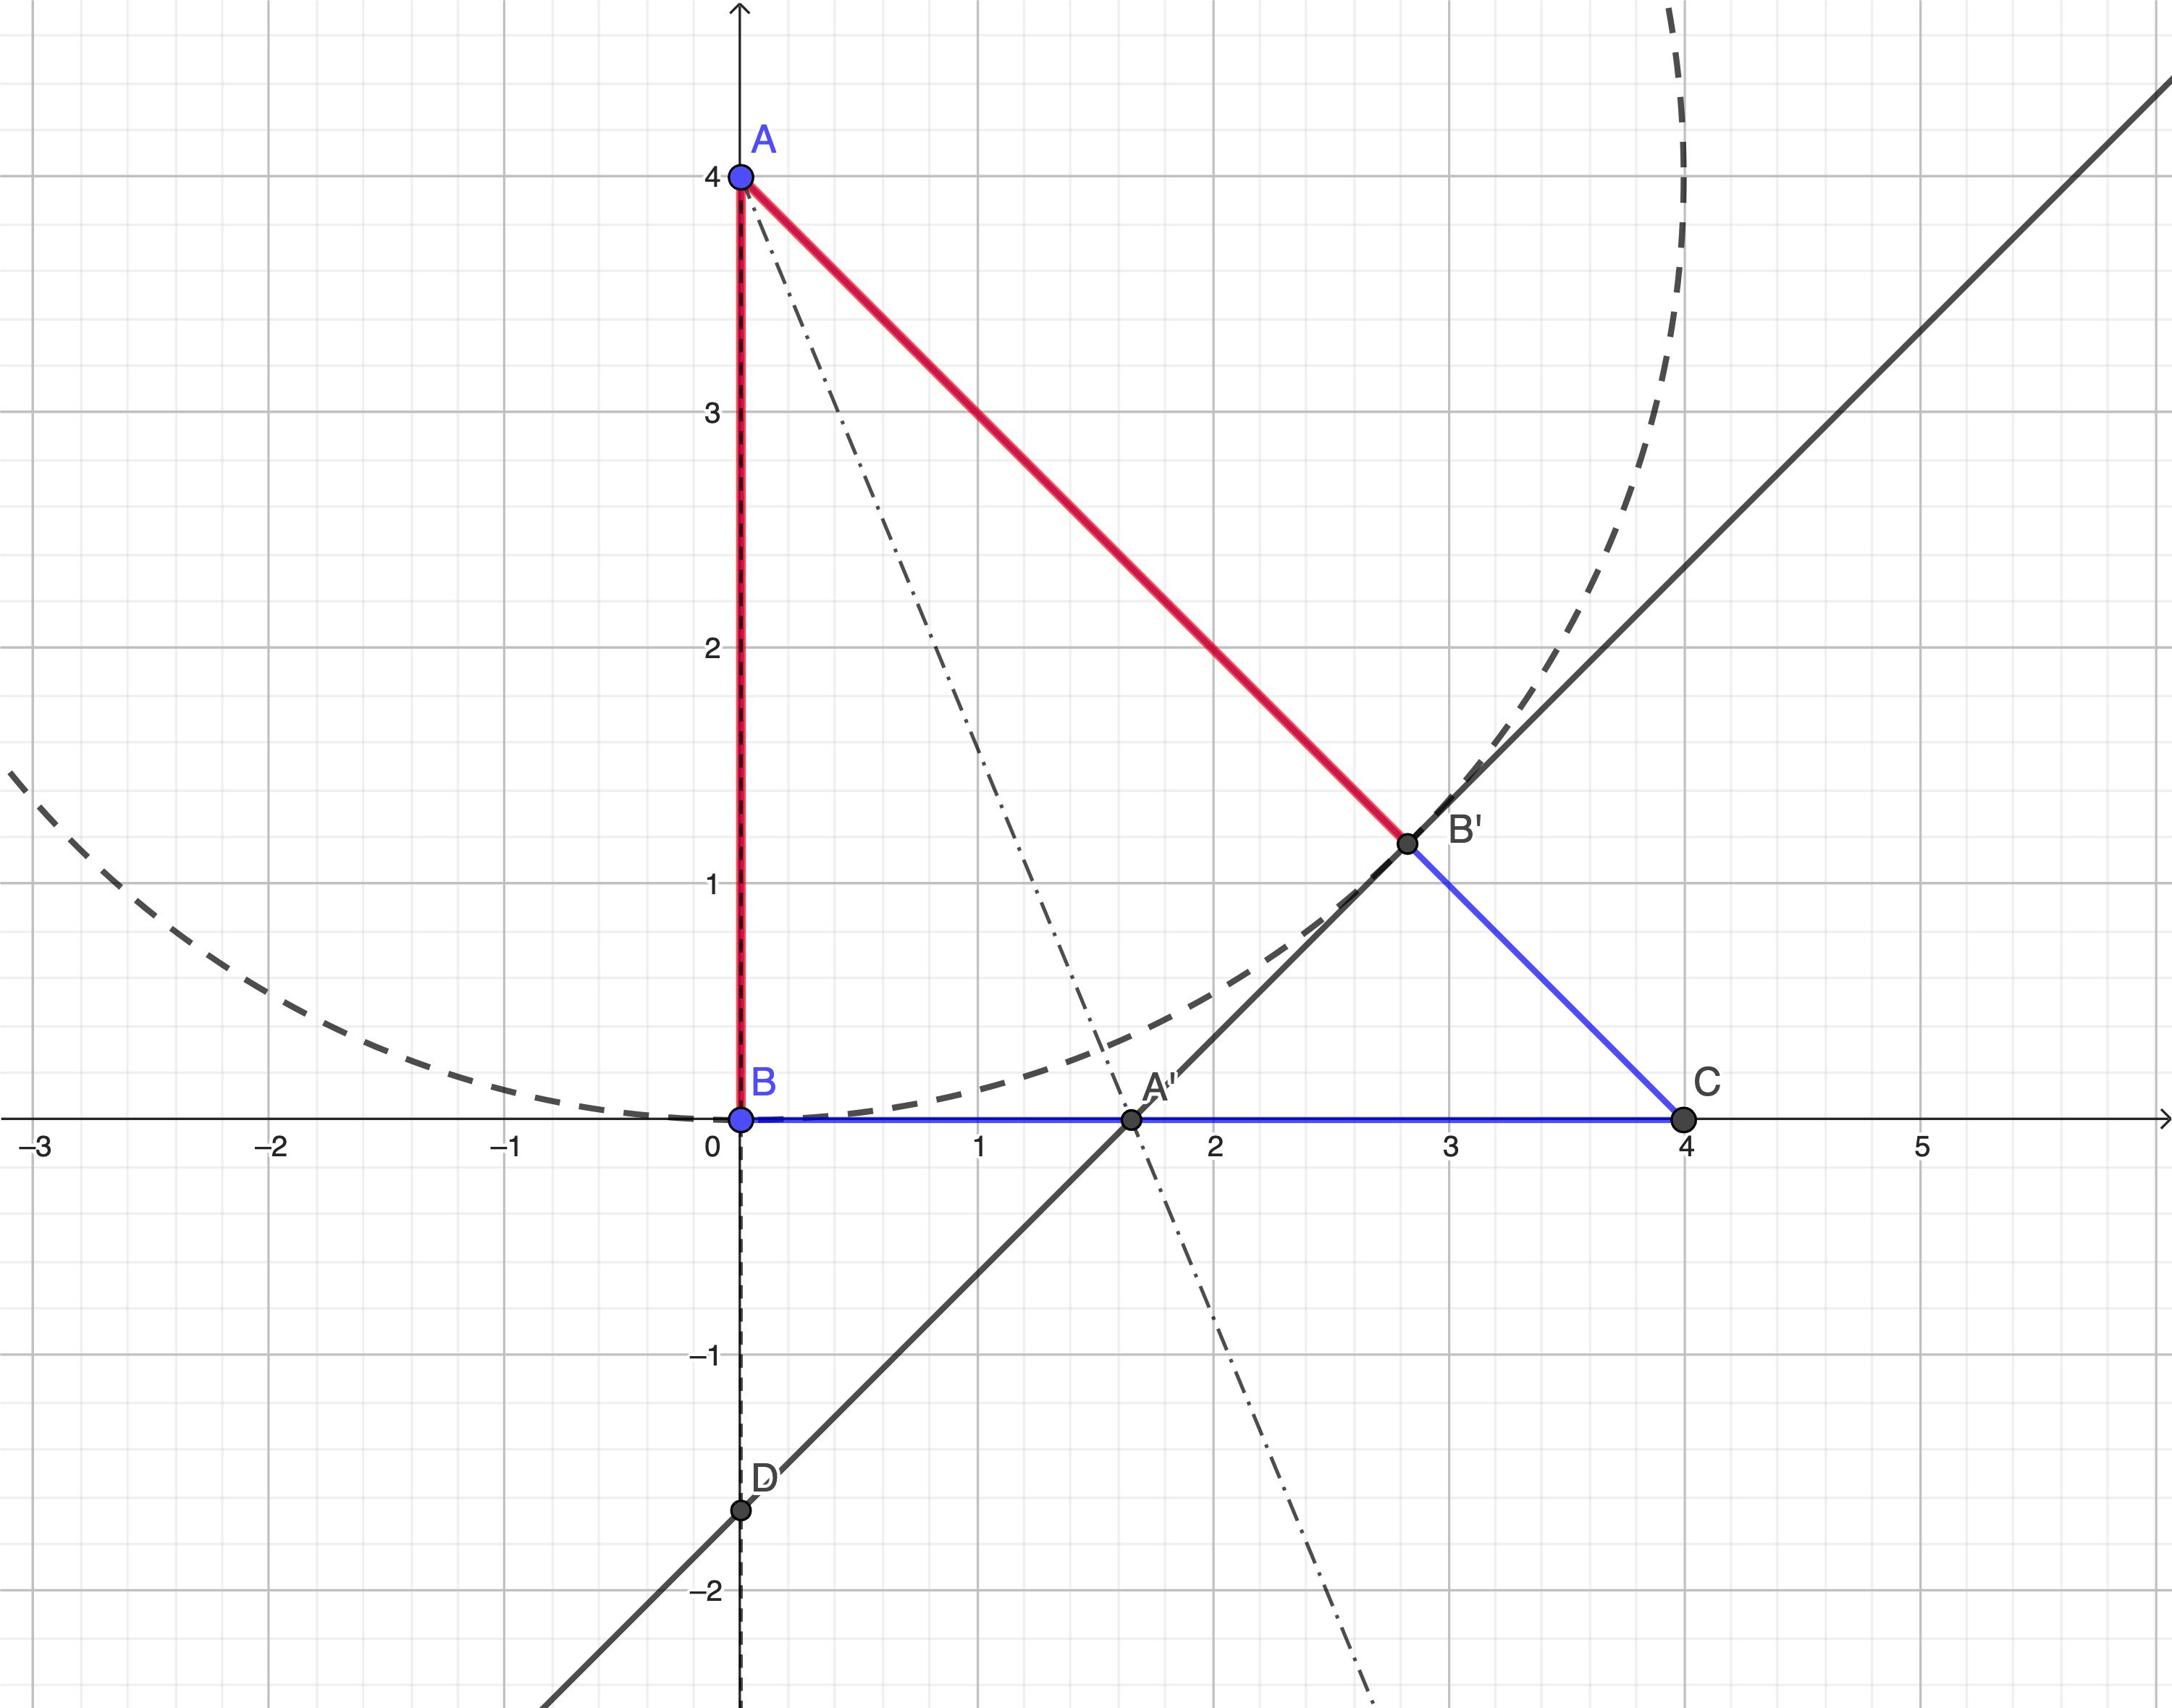
\includegraphics[width=.9\linewidth]{./manip_real/img/isorectangle-sqrt2-png.png}
\caption{Preuve géométrique de l'irrationalité de \(\sqrt{2}\)}
\end{figure}

\clearpage

\begin{itemize}
\item \hyperref[orgc112f4f]{Voir menu précédent}
page~\pageref{page:content6-menu}
\item \hyperref[orgb8d930f]{Voir section précédente}
page~\pageref{page:sec2.6.4irr}
\end{itemize}


\clearpage
\end{enumerate}

\section{Exercice 11}
\label{sec:orge303421}
\label{org1486a04}
\label{page:sec2.6.5exo11}

Considérons un cube d'arête 1.

\begin{enumerate}
\item Montrer que la diagonale principale (reliant deux sommets opposés
en traversant le cube) vaut exactement \(\sqrt{3}\).
\item Montrer que \(\sqrt{3}\) est irrationnel.
\end{enumerate}



\begin{itemize}
\item \hyperref[orgc0eae64]{Voir solution de l'exercice 11}
page~\pageref{page:sec8.6.2sol11}
\item \hyperref[orgc112f4f]{Voir menu précédent}
page~\pageref{page:content6-menu}
\item \hyperref[orgea5a5bb]{Voir section précédente}
page~\pageref{page:sqrt2proofs}
\end{itemize}


\clearpage

\section{Généralisation}
\label{sec:org96af429}
\label{org24a50ec}
\label{page:sec2.6.6gen}

Montrons par l'absurde\index{raisonnement!par l'absurde} que si \(p\)
est un nombre premier alors \(\sqrt{p}\) est
irrationnel.\index{ensemble!des nombres irrationnels}

Supposons par l'absurde que :

\[\sqrt{p} = \dfrac{a}{b}\]

avec

\[pgcd(a, b) = 1\]\index{pgcd}

Il vient :

\[a^2 = pb^2\]

or \(a^2\) et \(b^2\) n'ont pas de diviseur commun donc \(p\) divise
\(a^2\) et donc \(a\) (car \(p\) ne peut pas être un carré).

Ainsi \(a = pk\) avec \(k\in\mathbb{Z}\).

Par conséquent

\[a^2 = p^2k^2\]

et d'autre part

\[a^2 = pb^2\]

d'où

\[b^2 = pk^2\]

Puisque \(a^2\) et \(b^2\) n'ont pas de diviseur commun alors \(k^2\) ne
divise pas \(b^2\).

Donc c'est forcément \(p\) ce qui est absurde parce que cela contredit
l'hypothèse \(pgcd(a, b) = 1\).

\textbf{CQFD}

\newpage

En fait, que l'on choisisse \(k^2\) ou \(p\) comme diviseur de \(b^2\)
dans les deux cas on aboutit à une contradiction.

De plus, il y a un passage subtil ici, c'est parce que \(p\) est
premier\index{ensembles!des nombres premiers} (comme 2 et 3) que \(p\)
divise \(a^2\) entraîne \(p\) divise \(a\).


Prenez le nombre 4, il divise \(2^2\) mais ne divise pas \(2\). Ou
encore le nombre 9 qui divise \(6^2\) mais qui ne divise pas 6.

Donc la primalité de \(p\) est importante sinon la
démonstration\index{démonstration} est invalide.



\begin{itemize}
\item \hyperref[orgc112f4f]{Voir menu précédent}
page~\pageref{page:content6-menu}
\item \hyperref[org1486a04]{Voir section précédente}
page~\pageref{page:sec2.6.5exo11}
\end{itemize}


\clearpage

\section{Exercice 12}
\label{sec:org7db9ebf}
\label{org677ae69}
\label{page:sec2.6.7exo12}


\begin{enumerate}
\item Trouver 5 contre-exemples de nombres \(k\) qui divisent \(a^2\) mais
\(k\) qui ne divisent pas \(a\).
\item Montrer que \[\Phi = \dfrac{1 + \sqrt{5}}{2}\] est
irrationnel.\index{nombre!irrationnel}
\end{enumerate}



\begin{itemize}
\item \hyperref[org86d02ad]{Voir la solution de l'exercice 12}
page~\pageref{page:sec8.6.2sol11}
\item \hyperref[orgc112f4f]{Voir menu précédent}
page~\pageref{page:content6-menu}
\item \hyperref[org24a50ec]{Voir section précédente}
page~\pageref{page:sec2.6.6gen}
\end{itemize}


\clearpage

\section{Probablement irrationnel}
\label{sec:orga8d0f3b}
\label{org01d7b7d}
\label{page:sec2.6.8prob}


Aussi surprenant que cela puisse paraître il y a infiniment plus
de nombres irrationnels\index{ensemble!des nombres irrationnels} que
de rationnels.\index{ensemble!des nombres rationnels}

Si vous lanciez un couteau au hasard sur une planche en bois
graduée\footnote{Voir la figure page \pageref{page:real-line} pour voir
la droite des réels dont la planche en bois serait une illustration
concrète.}\ldots{}

\ldots{} vous tomberiez probablement sur un nombre irrationnel.

Malheureusement les mathématiques nécessaires pour
montrer\index{montrer} ce résultat dépasse largement le cadre de cet
ouvrage et du lycée en général. Il faudrait invoquer des arguments
d'analyse topologique à propos de la notion de densité.

Tout ça pour vous dire que l'aventure avec les nombres
réels\index{nombres!réels} (et les nombres en général) continue bien
au-delà des limites de ce livre.

Et c'est avec regret que je suis contraint de vous laissez sans preuve
pour l'irrationalité\index{ensemble!des nombres irrationnels} de
\(\pi\).

Voyez-vous, les arguments requis font appels aux concepts
de dérivée (que vous verrez en première), d'intégrale (que vous
verrez en terminale) et d'autres plus sophistiqués qui
interviendront dans les mathématiques du supérieur.

Espérons tout de même que la lecture de ce livre vous aura fait
découvrir la richesse des nombres réels. Si vous avez la moindre
suggestion d'amélioration merci de m'écrire à l'adresse
indiquée dans le formulaire avec pour objet : \textbf{Livre Manipuler les
réels}.

\begin{itemize}
\item \hyperref[orgc112f4f]{Voir menu précédent}
page~\pageref{page:content6-menu}
\item \hyperref[org677ae69]{Voir section précédente}
page~\pageref{page:sec2.6.7exo12}
\end{itemize}


\clearpage

\part{Capacités attendues}
\label{sec:orgb7098ab}
\label{org9c65356}
\label{page:sec3capacities}

\begin{myquote}{Sebastian Thrun}
\enquote{To me, mathematics, computer science, and the arts are insanely
related. They’re all creative expressions.}
\footnote{Consultez la page Wikipédia sur Thrun : \url{https://en.wikipedia.org/wiki/Sebastian_Thrun}}
\end{myquote}
\index{Thrun, Sebastian}


\clearpage

\label{orgb90956a}
\label{page:capacities-menu}
\begin{itemize}
\item \hyperref[org09fb152]{Rappels concernant les capacités attendues} page \pageref{page:sec3review}
\item \hyperref[org8554f1b]{Capacité \(C_1\)} page \pageref{page:sec3.2capacity1}
\item \hyperref[org3ab5664]{Capacité \(C_2\)} page \pageref{page:sec3.3capacity2}
\item \hyperref[org376c46d]{Capacité \(C_3\)} page \pageref{page:sec3.4capacity3}
\item \hyperref[org67b7ea7]{Capacité \(C_4\)} page \pageref{page:sec3.5capacity4}
\item \hyperref[org4fcdbf1]{Contenus} page \pageref{page:sec2contents}
\item \hyperref[org08a4120]{Démonstrations} page \pageref{page:sec4proofs}
\end{itemize}

\clearpage

\chapter{Rappels concernant les capacités attendues}
\label{sec:orgd0be93f}
\label{org09fb152}
\label{page:sec3review}

\begin{myquote}{Michel Demazure}
\enquote{Il n’y a guère de discipline plus mal connue et plus mal décrite
que la mathématique. Combien pourraient répondre à la question :
les mathématiques ça parle de quoi ? ça porte sur quoi ? ça propose
quel but ?}\footnote{Voir la page Wikipédia dédiée à Demazure : \url{https://fr.wikipedia.org/wiki/Michel_Demazure}}
\end{myquote}
\index{Demazure, Michel}


\clearpage

Pour rappels tous les codes sont accessibles sur Google Colab à
l'adresse communiquée dans la section concernée lorsque vous
aurez rempli ce petit formulaire : \url{https://forms.gle/qY8ym3ZxSo9NVH3S7}
(vous trouverez également les corrections de tous les exercices du
livre).

C'est également sur Google Colab que vous pourrez tester tous les
programmes qui vous permettent de pratiquer les capacités attendues
de manière interactive.


\begin{itemize}
\item \(C_1\) : << Associer à chaque point de la droite graduée un unique
nombre réel et réciproquement. >>
\item \(C_2\) : << Représenter un intervalle de la droite
numérique. Déterminer si un nombre réel appartient à un intervalle
donné. >>
\item \(C_3\) : << Donner un encadrement, d'amplitude\index{amplitude}
donnée, d'un nombre réel par des
décimaux\index{nombres!décimaux}. >>
\item \(C_4\) : << Dans le cadre de la résolution de problèmes, arrondir
en donnant le nombre de chiffres significatifs adapté à la situation
étudiée. >>
\end{itemize}


Tout ça se trouve sur Google Colab de façon interactive.

\clearpage

\chapter{Capacité \(C_1\)}
\label{sec:orgd137f12}
\label{org8554f1b}
\label{page:sec3.2capacity1}

\begin{myquote}{Stephan Banach}
\enquote{Un mathématicien est une personne capable de trouver des analogies
entre les théorèmes ; un meilleur mathématicien peut voir des
analogies entre les démonstrations. Les très bons mathématiciens
sont ceux capables de déceler des analogies entre des
théories. Mais on peut supposer que le mathématicien ultime est
celui qui peut voir des analogies entres les analogies.}
\footnote{Consulter la page Wikipédia consacrée à Banach : \url{https://fr.wikipedia.org/wiki/Stefan_Banach}}
\end{myquote}
\index{Banach, Stephan}

\clearpage


Cette partie développe la rubrique intitulée :

\(C_{1}\) : << Associer à chaque point de la droite graduée un unique
nombre réel et réciproquement. >>

dans le \href{https://eduscol.education.fr/document/24553/download}{programme officiel}\footnote{Consulter le programme officiel à cette adresse :
\url{https://eduscol.education.fr/document/24553/download}}.
\clearpage


\label{orgccf1b93}
\label{page:capacity1-menu}
\begin{itemize}
\item \hyperref[orgd1ad3aa]{Code pour construire les points} page \pageref{page:sec3.2.1pts}
\item \hyperref[org6da0729]{Exercice 13} page \pageref{page:sec3.2.2exo13}
\item \hyperref[orgb90956a]{Menu précédent} page \pageref{page:capacities-menu}
\item \hyperref[org3ab5664]{Capacité suivante} page \pageref{page:sec3.3capacity2}
\end{itemize}



\clearpage

\section{Code pour construire les points}
\label{sec:org6c5bc93}
\label{orgd1ad3aa}
\label{page:sec3.2.1pts}

Pour rappels tous les codes sont accessibles sur Google Colab à
l'adresse communiquée dans la section concernée lorsque vous
aurez rempli ce petit formulaire : \url{https://forms.gle/qY8ym3ZxSo9NVH3S7}
(vous trouverez également les corrections de tous les exercices du
livre).

C'est également sur Google Colab que vous pourrez tester tous les
programmes qui vous permettent de pratiquer les capacités attendues
de manière interactive.

Voici le code pour construire les points :

\clearpage

\begin{minted}[]{python}
import matplotlib.pyplot as plt
import numpy as np

c_1 = "Associer à chaque point de la droite "
c_1 += "graduée un unique nombre réel et "
c_1 += "réciproquement."
print(c_1)
numbers = [-2, -0.5, 0, 1, np.sqrt(2), np.pi]
labels = ['P_0', 'P_1', 'P_2', 'P_3', 'P_4', 'P_5']

plt.figure(figsize=(10, 1))

# Ploter une ligne horizontale
plt.plot(
    [min(numbers), max(numbers)],
    [0, 0],
    'k'
)

# Placer les nombres sur la ligne graduée
plt.scatter(
    numbers,
    np.zeros_like(numbers),
    color='red'
)

# Ajouter des étiquettes aux nombres
for i, label in enumerate(labels):
    plt.text(
        numbers[i],
        0.02,
        label, ha='center'
    )

# Masquer les axes
plt.axis('off')

plt.show()
\end{minted}

\begin{itemize}
\item \hyperref[orgccf1b93]{Voir menu précédent}
page~\pageref{page:capacity1-menu}
\end{itemize}


\clearpage


\section{Exercice 13}
\label{sec:orgfa7ff04}
\label{org6da0729}
\label{page:sec3.2.2exo13}

Voici le code pour lancer l'exercice :

\begin{minted}[]{python}
from math import pi

nombres = {2**0.5, -2, -0.5, 1, pi, 0}
points = {
  'P_0': 0, 'P_1': 0, 'P_2': 0,
  'P_3': 0, 'P_4': 0, 'P_5': 0
}
msg = "Voici la liste des points dont "
msg += "tu vas déterminer les abscisses"
print(msg)
print(points)

nb_msg = f"{round(nb, 4)} correspond à "
nb_msg += "l'abscisse de quel point ? "
for nb in nombres:
  p = input(nb_msg)
  points[p] = round(nb, 4)
\end{minted}

\begin{itemize}
\item \hyperref[orgcc6458f]{Voir solution de l'exercice 13}
page~\pageref{page:sec9.1.1sols13}
\item \hyperref[orgccf1b93]{Voir menu précédent}
page~\pageref{page:capacity1-menu}
\item \hyperref[orgd1ad3aa]{Voir section précédente}
page~\pageref{page:sec3.2.1pts}
\end{itemize}


\clearpage

\chapter{Capacité \(C_2\)}
\label{sec:orgb107152}
\label{org3ab5664}
\label{page:sec3.3capacity2}

\begin{myquote}{Jacques Hadamard}
\enquote{Le but de la rigueur mathématique est de sanctionner et de
légitimiser les conquêtes de l'intuition, et il n'y a  jamais eu
d'autre raison de la développer.}
\footnote{Lire la page Wikipédia sur Hadamard : \url{https://fr.wikipedia.org/wiki/Jacques_Hadamard}}
\end{myquote}
\index{Hadamard, Jacques}

\clearpage

Cette partie développe la rubrique intitulée :

\(C_{2}\) : << Représenter un intervalle de la droite numérique.
Déterminer si un nombre réel appartient à un intervalle donné. >>

dans le \href{https://eduscol.education.fr/document/24553/download}{programme officiel}\footnote{Lisez le programme officiel à l'adresse :
\url{https://eduscol.education.fr/document/24553/download}}.

\clearpage

\label{org449ea02}
\label{page:capacity2-menu}
\begin{itemize}
\item \hyperref[org873e05f]{Placement des abscisses sur la droite réelle} page
\pageref{page:sec3.3.1x-axis}
\item \hyperref[org7d5ffab]{Exercice 14} page \pageref{page:sec3.3.2exo14}
\item \hyperref[orgb90956a]{Menu précédent} page \pageref{page:capacities-menu}
\item \hyperref[org6da0729]{Section précédente} page \pageref{page:sec3.2.2exo13}
\item \hyperref[org8554f1b]{Capacité précédente} page \pageref{page:sec3.2capacity1}
\item \hyperref[org376c46d]{Capacité suivante} page \pageref{page:sec3.4capacity3}
\end{itemize}


\clearpage

\section{Placement des abscisses sur la droite réelle}
\label{sec:org4293055}
\label{org873e05f}
\label{page:sec3.3.1x-axis}

Pour rappels tous les codes sont accessibles sur Google Colab à
l'adresse communiquée dans la section concernée lorsque vous
aurez rempli ce petit formulaire : \url{https://forms.gle/qY8ym3ZxSo9NVH3S7}
(vous trouverez également les corrections de tous les exercices du
livre).

C'est également sur Google Colab que vous pourrez tester tous les
programmes qui vous permettent de pratiquer les capacités attendues
de manière interactive.

\clearpage

Voici le code :

\begin{minted}[]{python}
import matplotlib.pyplot as plt
import numpy as np

c_2 = "Représenter un intervalle de la "
c_2 += "droite numérique.\nDéterminer si " 
c_2 += "un nombre réel appartient à un "
c_2 += "intervalle donné."
print(c_2)
numbers = [1 + i/10 for i in range(11)]
labels = [str(num) for num in numbers]

plt.figure(figsize=(10, 1))

# Ploter une ligne horizontale
plt.plot(
    [min(numbers), max(numbers)],
    [0, 0],
    'k'
)

# Placer les nombres sur la ligne graduée
plt.scatter(
    numbers,
    np.zeros_like(numbers),
    color='red'
)

# Ajouter des étiquettes aux nombres
for i, label in enumerate(labels):
    plt.text(
        numbers[i],
        0.02,
        label, ha='center'
    )

# Masquer les axes
plt.axis('off')

plt.show()
\end{minted}

\begin{itemize}
\item \hyperref[org449ea02]{Voir menu précédent}
page~\pageref{page:capacity2-menu}
\end{itemize}

\clearpage

\section{Exercice 14}
\label{sec:org676b878}
\label{org7d5ffab}
\label{page:sec3.3.2exo14}

Pour rappels tous les codes sont accessibles sur Google Colab à
l'adresse communiquée dans la section concernée lorsque vous
aurez rempli ce petit formulaire : \url{https://forms.gle/qY8ym3ZxSo9NVH3S7}
(vous trouverez également les corrections de tous les exercices du
livre).

C'est également sur Google Colab que vous pourrez tester tous les
programmes qui vous permettent de pratiquer les capacités attendues
de manière interactive.

\clearpage

Voici le code pour générer l'exercice :

\begin{minted}[]{python}
num_to_square = [1 + i/10 for i in range(5)]
list_of_intervals = []


for n2s in num_to_square:
  msg = "Dans quel intervalle appartient "
  msg += f"{n2s}**2 ?"
  print(msg)

  interval = []


  for borne in ("inf", "sup"):
    msg = f"Borne {borne}érieure au "
    msg += "dixième = "
    interval.append(float(input(msg)))


  list_of_intervals.append(interval)




print("Voici la liste de tes réponses")
print(list_of_intervals)
print("Voici tes correspondances")


for i in range(len(num_to_square)):
  n2s = num_to_square[i]
  interval = list_of_intervals[i]
  msg = f"{n2s}**2 = {round(n2s**2, 2)} "
  msg += " appartient à "
  msg += f"l'intervalle {interval}"
  print(msg)
\end{minted}


\newpage

\begin{itemize}
\item \hyperref[orgfeec3ba]{Voir solution de l'exercice 14}
page~\pageref{page:sec9.2.1sol14}
\item \hyperref[org449ea02]{Voir menu précédent}
page~\pageref{page:capacity2-menu}
\item \hyperref[org873e05f]{Voir section précédente}
page~\pageref{page:sec3.3.1x-axis}
\end{itemize}


\clearpage

\chapter{Capacité \(C_3\)}
\label{sec:orga9c5ab5}
\label{org376c46d}
\label{page:sec3.4capacity3}

\begin{myquote}{Galilée}
\enquote{La physique est écrite dans cet immense livre qui continuellement
se tient ouvert devant nos yeux (je veux dire l'univers), mais elle
ne peut se comprendre si on ne s'exerce d'abord à comprendre la
langue et à connaître les caractères avec lesquels elle est
écrite. Elle est écrite en langue mathématique, et les caractères
sont les triangles, les cercles et autres figures géométriques,
sans lesquelles il est humainement impossible d'en comprendre le
moindre mot, sans lesquelles on s'égare vainement dans un
labyrinthe obscur.}\footnote{Voir la page Wikipédia sur Galilée : \url{https://fr.wikipedia.org/wiki/Galil\%C3\%A9e_\%28savant\%29}}
\end{myquote}
\index{Galilée}

\clearpage

Cette partie développe la rubrique intitulée :

\(C_{3}\) : << Donner un encadrement, d'amplitude\index{amplitude}
donnée, d'un nombre réel des décimaux\index{nombres!décimaux}. >>


dans le \href{https://eduscol.education.fr/document/24553/download}{programme officiel}\footnote{Pour consulter le programme officiel allez à l'adresse :
\url{https://eduscol.education.fr/document/24553/download}}.
\clearpage

\label{org67109aa}
\label{page:capacity3}
\begin{itemize}
\item \hyperref[org8cc10b8]{Exercice 15} page \pageref{page:sec3.4.1exo15}
\item \hyperref[org70c1962]{Exercice 16} page \pageref{page:sec3.4.2exo16}
\item \hyperref[orgb90956a]{Menu précédent} page \pageref{page:capacities-menu}
\item \hyperref[org7d5ffab]{Section précédente} page \pageref{page:sec3.3.2exo14}
\item \hyperref[org3ab5664]{Capacité précédente} page \pageref{page:sec3.3capacity2}
\item \hyperref[org67b7ea7]{Capacité suivante} page \pageref{page:sec3.5capacity4}
\end{itemize}



\clearpage

\section{Exercice 15}
\label{sec:orgb9ec665}
\label{org8cc10b8}
\label{page:sec3.4.1exo15}

Pour rappels tous les codes sont accessibles sur Google Colab à
l'adresse communiquée dans la section concernée lorsque vous
aurez rempli ce petit formulaire : \url{https://forms.gle/qY8ym3ZxSo9NVH3S7}
(vous trouverez également les corrections de tous les exercices du
livre).

C'est également sur Google Colab que vous pourrez tester tous les
programmes qui vous permettent de pratiquer les capacités attendues
de manière interactive.


Voici le code pour générer l'exercice :

\clearpage

\begin{minted}[]{python}
import math


some_primes = [
  2, 3, 5, 7, 11, 13,
  17, 19, 23, 31, 37, 41
]


prime_roots = [
  math.sqrt(sp) for sp in some_primes
]


for i in range(8, len(prime_roots)):
  inf = default(prime_roots[i], i)
  sup = excess(prime_roots[i], i)

  msg = "Un encadrement de "
  msg += f"sqrt({some_primes[i]}) ~"
  print(msg, end=" ")

  msg = f"{round(prime_roots[i], i)} "
  msg += f"d'amplitude 10**(-{i})"
  msg += " est :"
  print(msg, end=" ")

  msg = f"{inf} <= sqrt({some_primes[i]}) "
  msg += f"<= {sup}"
  print(msg)

  msg = "Dit autrement, "
  msg += "sqrt({some_primes[i]}) ~"
  print(msg, end=" ")

  msg = f"{round(prime_roots[i], i)}"
  print(msg, end=" ")

  msg = "appartient à l'intervalle "
  msg += "[{inf}; {sup}]"
  print(msg)




def exo_amplitude():
  score = 0
  method = [default, excess]
  born = ["inf", "sup"]
  motivation = "À toi de jouer !"
  print(motivation)
  instr = "Donne un encadrement à 10**"


  for i in range(5):
    msg = f"{instr}(-{some_primes[i]}) "
    msg += "près de "
    msg += f"sqrt({some_primes[i]})"
    print(msg)

    for j in range(2):
      t = method[j](
        prime_roots[i],
        some_primes[i]
      )

      msg = f"Borne {born[j]}érieure à "
      msg += f"{some_primes[i]} chiffres = "
      r = float(input(msg))
      if r == t:
        print("Bien joué !")
        score += 0.2
      else:
        print(f"La bonne réponse était {t}")
\end{minted}

\newpage

Pour rappels tous les codes sont accessibles sur Google Colab à
l'adresse communiquée dans la section concernée lorsque vous
aurez rempli ce petit formulaire : \url{https://forms.gle/qY8ym3ZxSo9NVH3S7}
(vous trouverez également les corrections de tous les exercices du
livre).

C'est également sur Google Colab que vous pourrez tester tous les
programmes qui vous permettent de pratiquer les capacités attendues
de manière interactive.


\begin{itemize}
\item \hyperref[orgb7308e1]{Voir solution de l'exercice 15}
page~\pageref{page:sec9.3.1-sol15}
\item \hyperref[org67109aa]{Voir menu précédent}
page~\pageref{page:capacity3}
\end{itemize}

\clearpage

\section{Exercice 16}
\label{sec:orgd834dec}
\label{org70c1962}
\label{page:sec3.4.2exo16}

Pour rappels tous les codes sont accessibles sur Google Colab à
l'adresse communiquée dans la section concernée lorsque vous
aurez rempli ce petit formulaire : \url{https://forms.gle/qY8ym3ZxSo9NVH3S7}
(vous trouverez également les corrections de tous les exercices du
livre).

C'est également sur Google Colab que vous pourrez tester tous les
programmes qui vous permettent de pratiquer les capacités attendues
de manière interactive.


Voici le code pour générer l'exercice :

\clearpage

\begin{minted}[]{python}
def approx_nums(some_numbers, decimals):
  score, method = 0, [default, excess]
  born = ["inf", "sup"]
  motivation = "À toi de jouer !"
  print(motivation)
  instr = "Donne un encadrement à 10**"

  for num in some_numbers:
    boundaries = [
      default(num, decimals),
      excess(num, decimals)
    ]

    msg = f"{instr}(-{decimals}) près de {num}"
    print(msg)


    for j in range(2):
      t = boundaries[j]
      msg = f"Borne {born[j]}érieure à "
      msg += f"{decimals} chiffres = "
      r = float(input(msg))
      if r == t:
        print("Bien joué !")
        score += 1
      else:
        print(f"La bonne réponse était {t}")


    x_pts = num
    inf, sup = boundaries[0], boundaries[1]
    d = decimals
    step = 10**(-decimals)

    zoom(
      x_pts,
      inf,
      sup,
      step,
      decimals,
      size=(9.75, 1.25)
    )


  msg = f"Score final = {score * 10}%"
  print(msg)



phi = (1 + 5**0.5) / 2 # nombre d'or
msg = "On appelle nombre d'or et on le note "
msg += r"\Phi = (1 + sqrt(5)) / 2 ~ "
msg += f"{phi}"
print(msg)

phi2, tau = phi**2, 2 * math.pi
msg = "Vous pouvez remarquer que "
msg += r"\Phi ** 2 = 1 + \Phi "
msg += "(vérifiez-le par le calcul !)"
print(msg)

msg = r"On appelle \tau = 2\pi ~ "
msg += f"{tau}"
print(msg)

msg = r"On ne présente plus \pi ~ "
msg += f"{math.pi}"
print(msg)

msg = "On appelle constante d'Euler "
msg += f"e ~ {math.e}"
print(msg)


some_numbers = [
  phi, phi2, math.e,
  math.pi, tau
]


decimals = random.randint(2, 5)
approx_nums(some_numbers, decimals)
\end{minted}

\newpage

Pour rappels tous les codes sont accessibles sur Google Colab à
l'adresse communiquée dans la section concernée lorsque vous
aurez rempli ce petit formulaire : \url{https://forms.gle/qY8ym3ZxSo9NVH3S7}
(vous trouverez également les corrections de tous les exercices du
livre).

C'est également sur Google Colab que vous pourrez tester tous les
programmes qui vous permettent de pratiquer les capacités attendues
de manière interactive.


\begin{itemize}
\item \hyperref[org2f710b4]{Voir solution de l'exercice 16}
page~\pageref{page:sec9.3.2sol16}
\item \hyperref[org67109aa]{Voir menu précédent}
page~\pageref{page:capacity3}
\item \hyperref[org8cc10b8]{Voir section précédente}
page~\pageref{page:sec3.4.1exo15}
\end{itemize}


\clearpage

\chapter{Capacité \(C_4\)}
\label{sec:orgfc1c1cd}
\label{org67b7ea7}
\label{page:sec3.5capacity4}

\begin{myquote}{André Weil}
\enquote{Tout mathématicien digne de ce nom a connu, parfois seulement à de
rares intervalles, ces états d’exaltation lucide où les pensées
s’enchaînent comme par miracle, et où l’inconscient (quel que soit
le sens qu’on attache à ce mot) paraît aussi avoir sa part. [...] A
la différence du plaisir sexuel, celui-là peut durer plusieurs
heures, voire plusieurs jours ; qui l’a connu en désire le
renouvellement mais est impuissant à le provoquer, sinon tout au
plus par un travail opiniâtre dont il apparaît alors comme la
récompense ; il est vrai que le plaisir qu’on en ressent est sans
rapport avec la valeur des découvertes auxquelles il s’associe.}
\footnote{Consulter la page Wikipédia sur Weil : \url{https://fr.wikipedia.org/wiki/Andr\%C3\%A9_Weil}}
\end{myquote}
\index{Weil, André}

\clearpage


Cette partie développe la rubrique intitulée :

\(C_{4}\) : << Dans le cadre de la résolution de problèmes, arrondir
en donnant le nombre de chiffres significatifs adapté à la situation
étudiée. >>

dans le \href{https://eduscol.education.fr/document/24553/download}{programme officiel}\footnote{Pour lire le programme officiel allez à l'adresse :
\url{https://eduscol.education.fr/document/24553/download}}.
\clearpage

\label{org7e69f0d}
\label{page:capacity5-menu}
\begin{itemize}
\item \hyperref[org4f79895]{Exercice 17} page \pageref{page:sec3.5.1exo17}
\item \hyperref[orgb90956a]{Menu précédent} page \pageref{page:capacities-menu}
\item \hyperref[org70c1962]{Section précédente} page \pageref{page:sec3.4.2exo16}
\item \hyperref[org376c46d]{Capacité précédente} page \pageref{page:sec3.4capacity3}
\item \hyperref[org08a4120]{Démonstrations} page \pageref{page:sec4proofs}
\end{itemize}





\clearpage

\section{Exemple}
\label{sec:org3698eeb}
\label{org9840e9a}
\label{page:sec3.5.0exemple}

Pour rappels tous les codes sont accessibles sur Google Colab à
l'adresse communiquée dans la section concernée lorsque vous
aurez rempli ce petit formulaire : \url{https://forms.gle/qY8ym3ZxSo9NVH3S7}
(vous trouverez également les corrections de tous les exercices du
livre).

C'est également sur Google Colab que vous pourrez tester tous les
programmes qui vous permettent de pratiquer les capacités attendues
de manière interactive.

\clearpage
Voici le code pour générer l'exemple :

\begin{minted}[]{python}
c = 299_792_458

msg = "La vitesse de la lumière dans le vide "
msg += f"est de {c} mètres par seconde."
print(msg)

e_s = "L'écriture scientifique d'un nombre "
e_s = "n = a x 10**k"
e_s += "\na appartient à l'intervalle "
e_s += "[1; 10[ donc a < 10"
e_s += "\nk appartient à l'ensemble des "
e_s += "entiers relatifs"

a, k = 2.99792458, 8

msg = "Son écriture scientifique est "
msg += f"c = {a} x 10**{k} m/s"
print(msg)

msg = "Pour passer des mètres aux kilomètres "
msg += "il faut diviser par 1 000"
print(msg)

msg = "Cela revient à multiplier par 10**(-3)"
print(msg)
msg = f"D'où c = {a} x 10**{k-3} km/s"
print(msg)

msg = "Dans 1 heure il y 60 minutes et "
msg += "dans 1 minute il y a 60 secondes"
print(msg)

msg = "Donc dans 1 heure il y a "
msg += "60 x 60 = 3600 secondes"
print(msg)

msg = "Donc il faut multiplier par 3600"
print(msg)

msg = "Mais dans ce cas, autant faire "
msg += "d'une pierre, deux coups"
print(msg)

msg = "Multiplier par 3600 et diviser par "
msg += "1 000 revient à multiplier par 3.6"
print(msg)

a *= 3.6


if a > 10:
  a /= 10
  k -= 1


print(f"D'où c = {a} x 10**{k} km/h")
\end{minted}

\begin{itemize}
\item \hyperref[org7e69f0d]{Voir menu précédent}
page~\pageref{page:capacity5-menu}
\end{itemize}


\clearpage

\section{Exercice 17}
\label{sec:org4cba4cc}
\label{org4f79895}
\label{page:sec3.5.1exo17}

Pour rappels tous les codes sont accessibles sur Google Colab à
l'adresse communiquée dans la section concernée lorsque vous
aurez rempli ce petit formulaire : \url{https://forms.gle/qY8ym3ZxSo9NVH3S7}
(vous trouverez également les corrections de tous les exercices du
livre).

C'est également sur Google Colab que vous pourrez tester tous les
programmes qui vous permettent de pratiquer les capacités attendues
de manière interactive.

\newpage

Voici le code pour générer l'exercice :

\begin{minted}[]{python}
print("À toi de jouer !")

mile = 1609.344

msg = f"Sachant que 1 mile = {mile} "
msg += "mètres"
print(msg)

msg = "Calcule la vitesse de la lumière "
msg += "en miles par heure."
print(msg)

msg = "Prend le temps de poser les "
msg += "calculs sur un papier avant de "
msg += "répondre"
print(msg.upper())

msg = "Vitesse en miles par heure = "
user_rep = float(input(msg))

msg = f"Selon toi c = {user_rep} mph "
msg += "(miles per hour)"
print(msg)
\end{minted}

\newpage

\begin{itemize}
\item \hyperref[orgef40258]{Voir solution de l'exercice 17}
page~\pageref{page:sec9.4.1sol17}
\item \hyperref[org7e69f0d]{Voir menu précédent}
page~\pageref{page:capacity5-menu}
\end{itemize}


\clearpage


\part{Démonstrations}
\label{sec:org0d2ae5c}
\label{org08a4120}
\label{page:sec4proofs}

\begin{myquote}{Bertrand Russell}
\enquote{Tout mathématicien digne de ce nom a connu, parfois seulement à de
rares intervalles, ces états d’exaltation lucide où les pensées
s’enchaînent comme par miracle, et où l’inconscient (quel que soit
le sens qu’on attache à ce mot) paraît aussi avoir sa part. [...] A
la différence du plaisir sexuel, celui-là peut durer plusieurs
heures, voire plusieurs jours ; qui l’a connu en désire le
renouvellement mais est impuissant à le provoquer, sinon tout au
plus par un travail opiniâtre dont il apparaît alors comme la
récompense ; il est vrai que le plaisir qu’on en ressent est sans
rapport avec la valeur des découvertes auxquelles il s’associe.}
\footnote{Lire l'excellente BD Logicomix qui retrace l'histoire
de la logique moderne via le regard de Bertrand Russell, consultez un
extrait gratuit sur Amazon : \url{https://amzn.to/41azKbz}}
\end{myquote}
\index{Russell, Bertrand}


\clearpage

\label{orgc52e956}
\label{page:proofs-menu}
\begin{itemize}
\item \hyperref[org3f97a9b]{Rappels des éléments du programme officiel} page \pageref{page:sec4.1review}
\item \hyperref[org6413964]{Démonstration numéro 1} page \pageref{page:sec4.2proof1}
\item \hyperref[org9c65356]{Capacités attendues} page \pageref{page:sec3capacities}
\item \hyperref[org091b4be]{Exemple d'algorithme} page \pageref{page:sec5algo}
\end{itemize}

\clearpage

\chapter{Rappels des éléments du \href{https://eduscol.education.fr/document/24553/download}{programme officiel}}
\label{sec:orgb9fafca}
\label{org3f97a9b}
\label{page:sec4.1review}




\begin{myquote}{David Hilbert}
\enquote{Une théorie mathématique ne peut être considérée comme complète
tant que l'on ne l'a clarifiée au point de pouvoir l'expliquer au
premier homme que l'on croise dans la rue.}
\footnote{Lire la page Wikipédia consacrée à Hilbert : \url{https://fr.wikipedia.org/wiki/David_Hilbert}}
\end{myquote}
\index{Hilbert, David}



\clearpage

Les deux démonstrations au \href{https://eduscol.education.fr/document/24553/download}{programme officiel}\footnote{Consulter le programme officiel à l'adresse :
\url{https://eduscol.education.fr/document/24553/download}} concernent :

\begin{itemize}
\item Le nombre rationnel \(\dfrac{1}{3}\) n'est pas décimal.
\item Le nombre réel \(\sqrt{2}\) est irrationnel.
\end{itemize}

Ces deux démonstrations sont traitées sur Google Colab.

Pour rappels tous les codes sont accessibles sur Google Colab à
l'adresse communiquée dans la section concernée lorsque vous
aurez rempli ce petit formulaire : \url{https://forms.gle/qY8ym3ZxSo9NVH3S7}
(vous trouverez également les corrections de tous les exercices du
livre).

\begin{itemize}
\item \hyperref[orgc52e956]{Voir menu précédent}
page~\pageref{page:proofs-menu}
\end{itemize}


\clearpage

\chapter{Démonstration numéro 1}
\label{sec:org0f2f2e8}
\label{org6413964}
\label{page:sec4.2proof1}

\begin{myquote}{Cédric Villani}
\enquote{Quel que soit le temps passé à faire des mathématiques, ce n'est
jamais du temps perdu.}
\footnote{Lisez la page Wikipédia de Villani : \url{https://fr.wikipedia.org/wiki/C\%C3\%A9dric_Villani}}
\end{myquote}
\index{Villani, Cédric}

\clearpage

Cette partie développe la rubrique intitulée :

<< Le nombre rationnel \(\dfrac{1}{3}\) n'est pas décimal. >>

du \href{https://eduscol.education.fr/document/24553/download}{programme officiel}\footnote{Lire le programme officiel à l'adresse :
\url{https://eduscol.education.fr/document/24553/download}}.

\clearpage


\label{orgfe369e8}
\label{page:proof1-menu}
\begin{itemize}
\item \hyperref[orga226baf]{À la main} page \pageref{page:sec4.2.1hand}
\item \hyperref[org498288d]{Avec Python} page \pageref{page:sec4.2.2python}
\item \hyperref[orgc52e956]{Menu précédent} page \pageref{page:proofs-menu}
\end{itemize}



\clearpage

\section{À la main}
\label{sec:orgcaec7fc}
\label{orga226baf}
\label{page:sec4.2.1hand}

Proposons une démonstration utilisant l'astuce des nombres à
décimales périodiques vue dans la section \hyperref[org36b98de]{Petite astuce}\footnote{Voir page \pageref{page:sec2.6.3tip}}.

Posons \[x = 0,3\dots 3\] où 3 se répète à l'infini. Multiplions par
10 puis retranchons \(x\).
Ainsi \[9x = 3\] donc \[x = \dfrac{1}{3}\]

\textbf{CQFD}

Pour \(\sqrt{2}\) consulter Google Colab ou les démonstrations
précédentes à la section \hyperref[orgea5a5bb]{Quelques preuves de l'irrationalité de
\(\sqrt{2}\)}. 

En espérant que la lecture de ce livre vous aura satisfait et fait
découvrir la richesse des nombres réels. Si vous avez la moindre
suggestion d'amélioration merci de m'écrire à l'adresse
indiquée dans le formulaire avec pour objet \textbf{Livre Manipuler les
réels}.

\begin{itemize}
\item \hyperref[orgfe369e8]{Voir menu précédent}
page~\pageref{page:proof1-menu}
\end{itemize}


\clearpage

\section{Avec Python}
\label{sec:org2bba363}
\label{org498288d}
\label{page:sec4.2.2python}

Pour rappels tous les codes sont accessibles sur Google Colab à
l'adresse communiquée dans la section concernée lorsque vous
aurez rempli ce petit formulaire : \url{https://forms.gle/qY8ym3ZxSo9NVH3S7}
(vous trouverez également les corrections de tous les exercices du
livre).

\clearpage

Voici le code pour générer les 3 démonstrations :

\begin{minted}[]{python}
def read_text(txt):
  for t in txt:
    msg = f"{t}\nAppuyez sur une touche pour "
    msg += "lire la suite..."
    input(msg)


intro = [
    "Le nombre 1/3 est-il décimal ?",
    "Pour que 1/3 soit décimal",
    "il faudrait trouver a et n tels que",
    "1/3 = a/10**n.",
    "En faisant 1 produit en croix on a ",
    "10**n = 3*a.",
    "Maintenant le problème devient ",
    "beaucoup plus simple.",
    "Il suffit de prouver qu'aucune ",
    "puissance de 10 n'est multiple de 3."
    ]

read_text(txt=intro)

multiple_of_3 = [3*k for k in range(21)]
print("Voici les multiples de 0 à 60")
print(multiple_of_3)

rem = input("Que remarquez-vous ? ")
msg = "Vous en voulez plus ? 0) Non 1) Oui\n"
more = input(msg)


if more == "1":
  for k in range(21, 50):
    print(3*k, end=", ")
  print()


msg = "Quels sont les diviseurs "
msg += "(entiers positifs) de 10 ? "

div = input(msg)
div = div.split(",")
div = [int(d) for d in div]

msg = f"Selon vous, les diviseurs de 10 sont {div}"
print(msg)

prime_proof = [
    "Les diviseurs de 10 sont 2 et 5",
    "Donc les diviseurs de n'importe ",
    "quelle puissance de 10",
    "sont de la forme 2**p x 5**q",
    "avec p et q tels que p + q <= n",
    "Aucune puissance de 2 ne divise 3",
    "car 2 et 3 sont premiers entre eux ",
    "(ils n'ont pas de diviseurs communs)",
    "il en va de même pour 5 et 3",
    "donc il est impossible d'obtenir 10**n = 3*a",
    "une autre façon de faire consiste à poser ",
    "la division de 10 par 3",
    "vous constaterez qu'il y aura toujours ",
    "un reste non nul",
    "et vous pourriez faire de même à l'infini "
    "avec toute puissance de 10"
]


read_text(txt=prime_proof)


div_proof = [
  f"10**{n} = 3 x {(10**n)//3} + {(10**n) % 3}"
  for n in range(10)
]

read_text(txt=div_proof)

decimal_proof = [
  f"1/3 ~ {round(1/3, i)} à {i} décimale(s)"
  for i in range(10)
]
read_text(txt=decimal_proof)

magic_proof = [
    "Supposons qu'il existe un nombre noté ",
    "x = 0.33...",
    "Puisqu'il y a une infinité de 3 alors",
    "10x = 3.333... ",
    "avec une infinité de 3 après la virgule",
    "10x - x = 3 ",
    "et donc 9x = 3 ",
    "d'où x = 3/9 = 1/3",
    "CQFD"
]
read_text(txt=magic_proof)
\end{minted}

\newpage

Pour rappels tous les codes sont accessibles sur Google Colab à
l'adresse communiquée dans la section concernée lorsque vous
aurez rempli ce petit formulaire : \url{https://forms.gle/qY8ym3ZxSo9NVH3S7}
(vous trouverez également les corrections de tous les exercices du
livre).


\begin{itemize}
\item \hyperref[orgfe369e8]{Voir menu précédent}
page~\pageref{page:proof1-menu}
\item \hyperref[orga226baf]{Voir section précédente}
page~\pageref{page:sec4.2.1hand}
\end{itemize}


\clearpage

\part{Exemple d'algorithme}
\label{sec:org272a3cb}
\label{org091b4be}
\label{page:sec5algo}

\begin{myquote}{Andrew Wiles}
\enquote{Just because we can’t find a solution, it doesn’t mean there isn’t
one.}
\footnote{Consultez la page de l'homme qui a démontré le grand théorème de Fermat : \url{https://en.wikipedia.org/wiki/Andrew_Wiles}}
\end{myquote}
\index{Wiles, Andrew}

\clearpage


\label{org3aca2a1}
\label{page:algos-menu}
\begin{itemize}
\item \hyperref[org06c5a30]{Rappel des éléments du programme officiel} page \pageref{page:sec5.1review}
\item \hyperref[org25f4c17]{Petites explications} page \pageref{page:sec5.2explain}
\item \hyperref[orgb14e38d]{Le code} page \pageref{page:sec5.3code}
\item \hyperref[org08a4120]{Démonstrations} page \pageref{page:sec4proofs}
\end{itemize}


\clearpage

\chapter{Rappel des éléments du \href{https://eduscol.education.fr/document/24553/download}{programme officiel}}
\label{sec:orgf010f67}
\label{org06c5a30}
\label{page:sec5.1review}



\begin{myquote}{Charles Gustave Jacob Jacobi}
\enquote{Monsieur Fourier avait l'opinion que le but principal des
mathématiques était l'utilité publique et l'explication des
phénomènes naturels. Un philosophe tel que lui aurait dû savoir que
le but unique de la Science, c'est l'honneur de l'esprit humain et
que, sous ce titre, une question de nombres vaut bien une question
de système du monde.}
\footnote{Lire la page Wikipédia dédiée à Jacobi : \url{https://fr.wikipedia.org/wiki/Charles_Gustave_Jacob_Jacobi}}
\end{myquote}
\index{Jacobi, Charles}


\clearpage

Le \href{https://eduscol.education.fr/document/24553/download}{programme officiel}\footnote{Adresse pour consulter le programme officiel :
\url{https://eduscol.education.fr/document/24553/download}} propose un seul exemple
d'algorithme :

\begin{itemize}
\item Déterminer par balayage un encadrement de \(\sqrt{2}\)
d'amplitude\index{amplitude} inférieure ou égale à \(10^{-n}\).
\end{itemize}


\begin{itemize}
\item \hyperref[org3aca2a1]{Voir menu précédent}
page~\pageref{page:algos-menu}
\end{itemize}

\clearpage

\chapter{Petites explications}
\label{sec:org08a872d}
\label{org25f4c17}
\label{page:sec5.2explain}

\begin{myquote}{René Descartes}
\enquote{Les mathématiques ont des inventions très subtiles et qui peuvent
beaucoup servir, tant à contenter les curieux qu'à faciliter tous
les arts et à diminuer le travail des hommes.}
\footnote{Voir la page Wikipédia sur Descartes : \url{https://fr.wikipedia.org/wiki/Ren\%C3\%A9_Descartes}}
\end{myquote}
\index{Descartes, René}


\clearpage

On cherche des réels \(a\) et \(b\) tels que :
\[a < \sqrt{2} < b\]
avec
\[\lvert a - b \rvert \leq 10^{-n}\]

Comme
\[\sqrt{2} \geq 1\]
alors on va choisir
\[a \geq 1\]

De sorte que :
\[a^2 \leq 2 \leq b^2\]

\begin{itemize}
\item \hyperref[org3aca2a1]{Voir menu précédent}
page~\pageref{page:algos-menu}
\item \hyperref[org06c5a30]{Voir section précédente}
page~\pageref{page:sec5.1review}
\end{itemize}

\clearpage

\chapter{Le code}
\label{sec:org89799dd}
\label{orgb14e38d}
\label{page:sec5.3code}

\begin{myquote}{Euclide}
\enquote{Si vous touchez aux maths, vous ne devez être ni pressés, ni
cupides, fussiez-vous roi ou reine.}
\footnote{Le chercheur français Christian Velpry a écrit un livre
très intéressant sur les origines africaines d'Euclide dont vous
pouvez lire un extrait gratuit sur Amazon : \url{https://amzn.to/46zlzAB}}
\end{myquote}
\index{Euclide}


\clearpage

Voici le code que vous pouvez retrouver sur Google Colab :

\begin{minted}[]{python}
def balayage(n):
  """
  Cette fonction renvoie les bornes
  d'un encadrement par balayage
  d'amplitude inférieure ou égale
  à 10**(-n)
  """
  a = 1
  b = a + 10**(-n)
  while b**2 < 2:
    a += 10**(-n)
    b = a + 10**(-n)
  return round(a, n), round(b, n)


# Tests : attention parce qu'au-delà de n = 7
# ça devient très long 
for n in range(1, 7):
  infimum, supremum = balayage(n)
  ampli = 10**(-n)
  msg = f"{infimum} < sqrt{2} < {supremum} "
  msg += "est un encadrement d'amplitude "
  msg += f"{ampli}"
  print(msg)
\end{minted}

\clearpage

Pour rappels tous les codes sont accessibles sur Google Colab à
l'adresse communiquée dans la section concernée lorsque vous
aurez rempli ce petit formulaire : \url{https://forms.gle/qY8ym3ZxSo9NVH3S7}
(vous trouverez également les corrections de tous les exercices du
livre).

En espérant que la lecture de ce livre vous aura satisfait et fait
découvrir la richesse des nombres réels. Si vous avez la moindre
suggestion d'amélioration merci de m'écrire à l'adresse
indiquée dans le formulaire avec pour objet \textbf{Livre Manipuler les
réels}.


\begin{itemize}
\item \hyperref[org3aca2a1]{Voir menu précédent}
page~\pageref{page:algos-menu}
\item \hyperref[org25f4c17]{Voir section précédente}
page~\pageref{page:sec5.2explain}
\end{itemize}


\clearpage

\part{Approfondissements possibles}
\label{sec:org61bb368}
\label{org2f59ee6}
\label{page:sec6deep}

\begin{myquote}{Bernard Baruch}
\enquote{Millions saw the apple fall, but Newton asked why.}
\footnote{Voir la page Wikipédia sur Baruch : \url{https://en.wikipedia.org/wiki/Bernard_Baruch}}
\end{myquote}
\index{Baruch, Bernard}




\clearpage

\label{org82a5705}
\label{page:deeps-menu}
\begin{itemize}
\item \hyperref[org1e7ea68]{Rappel des éléments du programme officiel} page \pageref{page:sec6.1review}
\item \hyperref[org419d7e0]{Petit bilan} page \pageref{page:sec6.2bilan}
\item \hyperref[orgde7e38b]{Et pour quelques exemples de plus} page \pageref{page:sec6.3exs}
\item \hyperref[org091b4be]{Exemple d'algorithme} page \pageref{page:sec5algo}
\item \hyperref[org16db6b7]{Après ce livre} page \pageref{page:sec7after}
\end{itemize}


\clearpage

\chapter{Rappel des éléments du \href{https://eduscol.education.fr/document/24553/download}{programme officiel}}
\label{sec:org207be03}
\label{org1e7ea68}
\label{page:sec6.1review}




\begin{myquote}{Isocrate}
\enquote{Les mathématiques sont une gymnastique de l'esprit et une
préparation à la philosophie.}
\footnote{Lire la page Wikipédia sur Isocrate : \url{https://fr.wikipedia.org/wiki/Isocrate}}
\end{myquote}
\index{Isocrate}

\clearpage
D'apprès le \href{https://eduscol.education.fr/document/24553/download}{programme officiel}\footnote{Adresse pour consulter le programme officiel :
\url{https://eduscol.education.fr/document/24553/download}} les approfondissements
possibles sont :

\begin{itemize}
\item Développement décimal illimité d'un nombre réel.
\item Observation, sur des exemples, de la périodicité du développement
décimal de nombres rationnels, du fait qu'un développement décimal
périodique correspond à un rationnel.
\end{itemize}


\begin{itemize}
\item \hyperref[org82a5705]{Voir menu précédent}
page~\pageref{page:deeps-menu}
\end{itemize}


\clearpage

\chapter{Petit bilan}
\label{sec:orga8b9a8b}
\label{org419d7e0}
\label{page:sec6.2bilan}

\begin{myquote}{William P. Thurston}
\enquote{Il y a une joie réelle à faire des mathématiques, à apprendre de
nouvelles méthodes de pensée qui expliquent, organisent et
simplifient. On peut ressentir cette joie en découvrant de
nouvelles mathématiques, (…) ou en trouvant une nouvelle façon
d’expliquer (…) une structure mathématique ancienne.}
\footnote{Consultez la page Wikipédia consacrée à Thurston : \url{https://en.wikipedia.org/wiki/William_Thurston}}
\end{myquote}
\index{Thurston, William}


\clearpage

\section{Développement décimal illimité d'un nombre réel}
\label{sec:org824dcb5}

Le développement décimal\index{développement décimal} illimité
d'un nombre réel est simplement son écriture avec une infinité de
chiffres après la virgule sans répétition régulière.

\clearpage

Considérons les quelques exemples suivants :

\begin{enumerate}
\item Le nombre \(\pi\) qui intervient pour calculer le périmètre
d'un cercle ou son aire : \[\pi \simeq 3,1415926536\dots\] est
approché à 10 décimales.
\item Le nombre d'or souvent noté \(\pi\) : \[\phi = \dfrac{1 +
       \sqrt{5}}{2} \simeq 1,6180339887\] est approché à 10 décimales.
\item Le nombre \(e\) d'\href{https://fr.wikipedia.org/wiki/Leonhard\_Euler}{Euler}\footnote{Lisez la page Wikipédia sur Euler à l'adresse :
\url{https://fr.wikipedia.org/wiki/Leonhard\_Euler}} qui sert de base à
l'exponentielle et sera abordé en classe de première
\[e \simeq 2,7182818285\dots\]
est approché à 10 décimales.
\item Le nombre \(\sqrt{2}\) qui représente la diagonale du carré de
côté 1 : \[\sqrt{2} \simeq 1,4142135624\dots\]
est approché à 10 décimales.
\item Le nombre \(\sqrt{3}\) qui représente la grande diagonale du
cube d'arête 1 : \[\sqrt{3} \simeq 1,7320508076\dots\]
est approché à 10 décimales (\hyperref[org1486a04]{voir l'exercice au sujet du cube}\footnote{Voir page \pageref{page:sec2.6.5exo11}}).
\end{enumerate}



\clearpage

Tous les nombres réels qui \textbf{NE} sont \textbf{PAS} rationnels connaissent
un déveleppement décimal illimité. Cela signifie qu'on ne pourra
jamais trouver de régularité dans leurs décimales contrairement
aux rationnels qui eux ont un développement périodique.


\begin{itemize}
\item \hyperref[org82a5705]{Voir menu précédent}
page~\pageref{page:deeps-menu}
\item \hyperref[org1e7ea68]{Voir section précédente}
page~\pageref{page:sec6.1review}
\end{itemize}


\clearpage

\section{Périodicité du développement décimal d'un nombre rationnel}
\label{sec:orgd80a238}

Pour le deuxième point on a déjà vu beaucoup d'exemples (cf la
petite astuce vue dans la section \hyperref[org36b98de]{Petite astuce}\footnote{Voir page \pageref{page:sec2.6.3tip}\}}).



Mais rien que pour le plaisir en voici encore un.

Soit \[x = 0,2023\dots\]
Ici la période est 2023.

Donc on va multiplier par \(10^4\) puis retrancher \(x\) d'où

\[9999x = 2023\]

qui entraîne

\[x = \dfrac{2023}{9999} \simeq 0,2023\dots 2023\dots\]



\begin{itemize}
\item \hyperref[org82a5705]{Voir menu précédent}
page~\pageref{page:deeps-menu}
\item \hyperref[org1e7ea68]{Voir section précédente}
page~\pageref{page:sec6.1review}
\end{itemize}



\clearpage

\chapter{Et pour quelques exemples de plus}
\label{sec:org54329ff}
\label{orgde7e38b}
\label{page:sec6.3exs}

\begin{myquote}{Albert Einstein}
\enquote{Pure mathematics is, in its way, the poetry of logical ideas.}
\footnote{Voir la page Wikipédia dédiée à Einstein : \url{https://en.wikipedia.org/wiki/Albert_Einstein}}
\end{myquote}
\index{Einstein, Albert}



\clearpage

Voici quelques développement décimaux\index{décimaux} illimités de
nombres réels :



\begin{itemize}
\item D1) : \[\sqrt{2} \simeq 1,414213562373095\dots\]
\item D2) : \[\Phi \simeq 1.618033988749895\dots\]
\item D3) : \[\sqrt{3} \simeq 1.7320508075688772\dots\]
\item D4) : \[\sqrt{5} \simeq 2.23606797749979\dots\]
\item D5) : \[\sqrt{7} \simeq 2.6457513110645907\dots\]
\item D6) : \[e \simeq 2.718281828459045\dots\]
\item D7) : \[\pi \simeq 3.141592653589793\dots\]
\item D8) : \[\sqrt{11} \simeq 3.3166247903554\dots\]
\end{itemize}


En espérant que la lecture de ce livre vous aura satisfait et fait
découvrir la richesse des nombres réels. Si vous avez la moindre
suggestion d'amélioration merci de m'écrire à l'adresse
indiquée dans le formulaire avec pour objet \textbf{Livre Manipuler les
réels}.


\begin{itemize}
\item \hyperref[org82a5705]{Voir menu précédent}
page~\pageref{page:deeps-menu}
\item \hyperref[org419d7e0]{Voir section précédente}
page~\pageref{page:sec6.2bilan}
\end{itemize}


\clearpage

\part{Après ce livre}
\label{sec:org5cc24aa}
\label{org16db6b7}
\label{page:sec7after}

\begin{myquote}{Alvin E. Roth}
\enquote{I’ve always been interested in using mathematics to make the world
work better.}
\footnote{Voir la page Wikipédia dédiée à Roth : \url{https://en.wikipedia.org/wiki/Alvin_E._Roth}}
\end{myquote}
\index{Roth, Alvin}


\clearpage

\label{org71f8d0a}
\label{page:after-menu}
\begin{itemize}
\item \hyperref[orgc860eab]{Conclusion} page \pageref{page:sec7.1conclusion}
\item \hyperref[org2f59ee6]{Approfondissements possibles} page \pageref{page:sec6deep}
\item \hyperref[orge8af971]{Solutions des exercices des contenus} page \pageref{page:sec8sols-contents}
\end{itemize}

\clearpage

\chapter{Conclusion}
\label{sec:org2af2cef}
\label{orgc860eab}
\label{page:sec7.1conclusion}

\begin{myquote}{Shakuntala Devi}
\enquote{Without mathematics, there’s nothing you can do. Everything around
you is mathematics. Everything around you is numbers.}
\footnote{Voir la page Wikipédia sur Devi : \url{https://en.wikipedia.org/wiki/Shakuntala_Devi}}
\end{myquote}
\index{Devi, Shakuntala}

\clearpage

Bravo à vous si vous avez lu jusqu'au bout.

Pour rappels tous les codes sont accessibles sur Google Colab à
l'adresse communiquée dans la section concernée lorsque vous
aurez rempli ce petit formulaire : \url{https://forms.gle/qY8ym3ZxSo9NVH3S7}
(vous trouverez également les corrections de tous les exercices du
livre).

Sur Google Colab vous pourrez expérimenter avec des exercices
nouveaux à chaque exécution du code. Cela vous permettra de vous
entraîner avec des valeurs différentes à chaque fois. C'est beaucoup
plus interactif que tous les exemples de ce livre.

Le but de ce livre est de vous donner un aperçu du monde merveilleux
des nombres réels. Mais il y a encore beaucoup de choses à découvrir
que je n'ai même pas pu mentionner ici.

Je vous invite à mettre le maximum d'étoiles sur Amazon et à laisser
un commentaire pour aider les gens qui cherchent des ressources utiles.

En espérant que la lecture de ce livre vous aura satisfait et fait
découvrir la richesse des nombres réels. Si vous avez la moindre
suggestion d'amélioration merci de m'écrire à l'adresse
indiquée dans le formulaire avec pour objet \textbf{Livre Manipuler les
réels}.

\begin{itemize}
\item \hyperref[org71f8d0a]{Voir menu précédent}
page~\pageref{page:after-menu}
\end{itemize}

\clearpage

\part{Solutions des exercices des contenus}
\label{sec:org3ec29c0}
\label{orge8af971}
\label{page:sec8sols-contents}

\begin{myquote}{Paul Richard Halmos}
\enquote{The only way to learn mathematics is to do mathematics.}
\footnote{Lire la page Wikipédia sur Halmos : \url{https://en.wikipedia.org/wiki/Paul_Halmos}}
\end{myquote}
\index{Halmos, Paul}


\clearpage

\label{orgd150cd0}
\label{page:sols-contents-menu}
\begin{itemize}
\item \hyperref[orgdc6a2eb]{Solutions des exercices du contenu 1} page \pageref{page:sec8.1sols-cont1}
\item \hyperref[org56f3479]{Solutions des exercices du contenu 2} page \pageref{page:sec8.2sols-cont2}
\item \hyperref[org76d02b6]{Solutions des exercices du contenu 3} page \pageref{page:sec8.3sols-cont3}
\item \hyperref[org74bc845]{Solutions des exercices du contenu 4} page \pageref{page:sec8.4sols-cont4}
\item \hyperref[orge89e966]{Solutions des exercices du contenu 5} page \pageref{page:sec8.5sols-cont5}
\item \hyperref[org4cedc13]{Solutions des exercices du contenu 6} page \pageref{page:sec8.6sols-cont6}
\item \hyperref[org16db6b7]{Après ce livre} page \pageref{page:sec7after}
\item \hyperref[orgd241bdf]{Solutions des exercices des capacités attendues} page
\pageref{page:sec9sols-capacities}
\end{itemize}




\clearpage

\chapter{Solutions des exercices du contenu 1}
\label{sec:org9b4c6c5}
\label{orgdc6a2eb}


\label{page:sec8.1sols-cont1}

\begin{myquote}{Creola Katherine Coleman}
\enquote{We will always have STEM with us. Some things will drop out of the
public eye and go away, but there will always be science,
engineering, and technology. And there will always, always be
mathematics.}
\footnote{Lire la page sur Coleman-Johnson qui a inspiré le film
<< les figures de l'ombre >> : \url{https://en.wikipedia.org/wiki/Katherine_Johnson}}
\end{myquote}
\index{Coleman, Creola}


\clearpage

\label{orgecd4f02}
\label{page:sols-cont1-menu}
\begin{itemize}
\item \hyperref[org51c56ef]{Solution de l'exercice 1} page \pageref{page:sec8.1.1sol1}
\item \hyperref[orged5d56d]{Solution de l'exercice 2 : Python} page \pageref{page:sec8.1.2sol2}
\item \hyperref[orgd150cd0]{Menu précédent} page \pageref{page:sols-contents-menu}
\item \hyperref[org56f3479]{Solutions des exercices du contenu 2} page \pageref{page:sec8.2sols-cont2}
\end{itemize}


\clearpage

\section{Solution de l'exercice 1}
\label{sec:orgacd1181}
\label{org51c56ef}
\label{page:sec8.1.1sol1}
On reprend le \hyperref[org084e38f]{même schéma}\footnote{Voir page \pageref{page:sec2.1.6cp}} que dans l'exemple.
\begin{itemize}
\item \(A = (x < -1)\)
\item \(B = (-3x > 3)\)
\item \(P = (A\Rightarrow B)\)
\item \(\neg B = (-3x \leq 3)\)
\item \(\neg A = (x \geq -1)\)
\item \(CP(P) = (\neg B\Rightarrow \neg A)\)
\end{itemize}


\begin{itemize}
\item \hyperref[orgfd91183]{Voir énoncé de l'exercice 1}
page~\pageref{page:sec2.1.7exo1}
\end{itemize}

\clearpage

\section{Solution de l'exercice 2 : Python}
\label{sec:org8f99e33}
\label{orged5d56d}
\label{page:sec8.1.2sol2}

\begin{enumerate}
\item Pour rappels tous les codes sont accessibles sur Google Colab à
l'adresse communiquée dans la section concernée lorsque vous aurez
rempli ce petit formulaire : \url{https://forms.gle/qY8ym3ZxSo9NVH3S7}
(vous trouverez également les corrections de tous les exercices du
livre).
Voici le code de la fonction \texttt{imply} :
\begin{minted}[]{python}
def imply(A, B):
   """
   Cette fonction prend 2 paramètres
   A et B en entrée et renvoie la
   phrase logique A implique B
   """
   return f"({A}) implique ({B})"

# Tests
A = ["x > 2", "x < -1"]
B = ["2*x > 4", "-3*x > 3"]
for i in range(len(A)):
   print(imply(A[i], B[i]))

# Sorties
# (x > 2) implique (2*x > 4)
# (x < -1) implique (-3*x > 3)
\end{minted}
\item Pour rappels tous les codes sont accessibles sur Google Colab à
l'adresse communiquée dans la section concernée lorsque vous aurez
rempli ce petit formulaire :
\url{https://forms.gle/qY8ym3ZxSo9NVH3S7} (vous trouverez également les
corrections de tous les exercices du livre).
Voici le code de la fonction \texttt{contrapose} : 
\begin{minted}[]{python}
def contrapose(A, B):
  """
  Cette fonction prend 2 paramètres
  A et B en entrée et renvoie la
  phrase logique non B implique non A
  """
  return imply("non " + B, "non " + A)

# Tests
A = ["x > 2", "x < -1"]
B = ["2*x > 4", "-3*x > 3"] 
for i in range(len(A)):
  print(contrapose(A[i], B[i]))

# Sorties
#(non 2*x > 4) implique (non x > 2)
#(non -3*x > 3) implique (non x < -1)
\end{minted}

\item \hyperref[orgce66a51]{Voir énoncé de l'exercice 2}
page~\pageref{page:sec2.1.8exo2}
\end{enumerate}

\clearpage

\chapter{Solutions des exercices du contenu 2}
\label{sec:orge2a9ff2}
\label{org56f3479}
\label{page:sec8.2sols-cont2}

\begin{myquote}{Richard Courant}
\enquote{Mathematics as an expression of the human mind reflects the active
will, the contemplative reason, and the desire for aesthetic
perfection. Its basic elements are logic and intuition, analysis
and construction, generality and individuality.}
\footnote{Voir la page Wikipédia sur Courant : \url{https://en.wikipedia.org/wiki/Richard_Courant}}
\end{myquote}
\index{Courant, Richard}

\clearpage

\label{orgd5de19a}
\label{page:sols-cont2}
\begin{itemize}
\item \hyperref[org34f5627]{Solution de l'exercice 3} page \pageref{page:sec8.2.1sol3}
\item \hyperref[orgea731a5]{Solution de l'exercice 4} page \pageref{page:sec8.2.2sol4}
\item \hyperref[org727e50c]{Solution du petit jeu} page \pageref{page:sec8.2.3sol-game}
\item \hyperref[orgd150cd0]{Menu précédent} page \pageref{page:sols-contents-menu}
\item \hyperref[orgdc6a2eb]{Solutions des exercices du contenu 1} page \pageref{page:sec8.1sols-cont1}
\item \hyperref[org76d02b6]{Solutions des exercices du contenu 3} page \pageref{page:sec8.3sols-cont3}
\end{itemize}

\clearpage

\section{Solution de l'exercice 3}
\label{sec:org5710084}
\label{org34f5627}
\label{page:sec8.2.1sol3}

\begin{enumerate}
\item \[\dfrac{1}{3}\in I_1 = [0,3 ; 0,4]\]
qui a pour amplitude\index{amplitude} :
\[|I_1| = 0,4 - 0,3 = 0,1 = 10^{-1}\]
\[\dfrac{1}{3}\in I_2 = [0,33 ; 0,34]\]
qui a pour amplitude :
\[|I_2| = 0,34 - 0,33 = 0,01 = 10^{-2}\]
\[\dfrac{1}{3}\in I_3 = [0,333 ; 0,334]\]
qui a pour amplitude :
\[|I_3| = 0,334 - 0,333 = 0,001 = 10^{-3}\]
On peut classer ces intervalles :
\[\dfrac{1}{3}\in I_3 = [0,333 ; 0,334] \subset I_2 = [0,33 ;
   0,34] \subset I_1 = [0,3 ; 0,4]\]
\item \[\sqrt{2}\in R_1 = [1,4 ; 1,5]\]
qui a pour amplitude :
\[|R_1| = 1,5 - 1,4 = 0,1 = 10^{-1}\]
\[\sqrt{2}\in R_2 = [1,41 ; 1,42]\]
qui a pour amplitude :
\[|R_2| = 1,42 - 1,41 = 0,01 = 10^{-2}\]
\[\sqrt{2}\in R_3 = [1,414 ; 1,415]\]
qui a pour amplitude :
\[|R_3| = 1,415 - 1,414 = 0,001 = 10^{-3}\]
On peut classer ces intervalles :
\[\sqrt{2}\in R_3 = [1,414 ; 1,415] \subset R_2 = [1,41 ;
   1,42]\subset R_1 = [1,4 ; 1,5]\]
\item \[\Phi = \dfrac{1 + \sqrt{5}}{2}\in F_1 = [1,6 ; 1,7]\]
qui pour amplitude :
\[|F_1| = 1,7 - 1,6 = 0,1 = 10^{-1}\]
\[\Phi = \dfrac{1 + \sqrt{5}}{2}\in F_2 = [1,61 ; 1,62]\]
qui pour amplitude :
\[|F_2| = 1,62 - 1,61 = 0,01 = 10^{-2}\]
\[\Phi = \dfrac{1 + \sqrt{5}}{2}\in F_3 = [1,618 ; 1,619]\]
qui pour amplitude :
\[|F_3| = 1,619 - 1,618 = 0,001 = 10^{-3}\]
On peut classer ces intervalles :
\[\Phi\in F_3 = [1,618 ; 1,619] \subset F_2 = [1,61 ; 1,62]\subset
   F_1 = [1,6 ; 1,7]\]
\item \[\pi\in P_1 = [3,1 ; 3,2]\]
qui a pour amplitude :
\[|P_1| = 3,2 - 3,1 = 0,1 = 10^{-1}\]
\[\pi\in P_2 = [3,14 ; 3,15]\]
qui a pour amplitude :
\[|P_2| = 3,15 - 3,14 = 0,01 = 10^{-2}\]
\[\pi\in P_3 = [3,141 ; 3,142]\]
qui a pour amplitude :
\[|P_3| = 3,142 - 3,141 = 0,001 = 10^{-3}\]
On peut classer ces intervalles :
\[\pi\in P_3 = [3,141 ; 3,142]\subset P_2 = [3,14 ; 3,15]\subset P_1 = [3,1 ;
   3,2]\]
\item \[\tau = 2\pi\in T_1 = [6,2 ; 6,3]\]
qui a pour amplitude :
\[|T_1| = 6,3 - 6,2 = 0,1 = 10^{-1}\]
\[\tau = 2\pi\in T_2 = [6,28 ; 6,29]\]
qui a pour amplitude :
\[|T_2| = 6,29 - 6,28 = 0,01 = 10^{-2}\]
\[\tau = 2\pi\in T_3 = [6,283 ; 6,284]\]
qui a pour amplitude :
\[|T_3| = 6,284 - 6,283 = 0,001 = 10^{-3}\]
On peut classer ces intervalles :
\[\tau = 2\pi\in T_3 = [6,283 ; 6,284]\subset T_2 = [6,28 ;
   6,29]\subset T_1 = [6,2 ; 6,3]\]

\item \hyperref[org61fbd6f]{Voir l'énoncé de l'exercice 3}
page~\pageref{page:sec2.2.2exo3}
\end{enumerate}

\clearpage

\section{Solution de l'exercice 4}
\label{sec:orgc506e60}
\label{orgea731a5}
\label{page:sec8.2.2sol4}


\begin{enumerate}
\item \[\Phi = \dfrac{1 + \sqrt{5}}{2} \simeq 1,61803\]
\item Voici les 16 premiers termes de cette suite de nombres :
\begin{itemize}
\item \[F_1 = 1,\quad F_2 = 1,\quad F_3 = 2,\quad F_4 = 3\]
\item \[F_5 = 5,\quad F_6 = 8,\quad F_7 = 13,\quad F_8 = 21\]
\item \[F_9 = 34,\quad F_{10} = 55,\quad F_{11} = 89,\quad F_{12} = 144\]
\item \[F_{13} = 233,\quad F_{14} = 377,\quad F_{15} = 610,\quad F_{16} = 987\]
\end{itemize}
\item Pour calculer un nouveau terme on ajoute les deux termes précédents
\[F_n = F_{n - 1} + F_{n-2}\]
Par exemple :
\[F_3 = F_2 + F_1 = 1 + 1 = 2\]
ou encore :
\[F_7 = F_6 + F_5 = 8 + 5 = 13\]
\begin{itemize}
\item \[\dfrac{F_2}{F_1} = 1,\quad \dfrac{F_3}{F_2} = 2\]
\item \[\dfrac{F_4}{F_3} = \dfrac{3}{2},\quad \dfrac{F_5}{F_4} = \dfrac{5}{3}\simeq 1,67\]
\item \[\dfrac{F_6}{F_5} = \dfrac{6}{5} = 1,2,\quad\dfrac{F_7}{F_6} = \dfrac{13}{8} = 1,625\]
\item \[\dfrac{F_8}{F_7} = \dfrac{21}{13}\simeq 1,615,\quad\dfrac{F_9}{F_8}\simeq 1,619\]
\item \[\dfrac{F_{10}}{F_9} = \dfrac{55}{34}\simeq 1,6176,\quad\dfrac{F_{11}}{F_{10}} = \dfrac{89}{55} = 1,6182\]
\end{itemize}
\item Les 11 premiers termes de la suites de Fibonacci ont permis
d'approcher le nombre d'or à 3 chiffres après la
virugle. Poursuivons avec ce que nous avons déjà calculer à la question 2.
\begin{itemize}
\item \[\dfrac{F_{12}}{F_{11}} = \dfrac{144}{89}\simeq 1,6180,\quad\dfrac{F_{13}}{F_{12}} = \dfrac{233}{144}\simeq 1,61801\]
\item \[\dfrac{F_{14}}{F_{13}} = \dfrac{377}{233}\simeq 1,61803,\quad\dfrac{F_{15}}{F_{14}} = \dfrac{610}{377}\simeq 1,61804\]
\end{itemize}
\[\Phi = \dfrac{1 + \sqrt{5}}{2} \simeq 1,61803\in
   \left[\dfrac{F_{14}}{F_{13}} ; \dfrac{F_{15}}{F_{14}}\right]\]
\end{enumerate}


\begin{itemize}
\item \hyperref[org6c6db0c]{Voir l'énoncé de l'exercice 4}
page~\pageref{page:sec2.2.3exo4}
\end{itemize}


\clearpage

\section{Solution du petit jeu}
\label{sec:orgcd21d5e}
\label{org727e50c}
\label{page:sec8.2.3sol-game}
\clearpage

\begin{enumerate}
\item Partie 1
\label{sec:orgb463b7d}

Voilà pour la première partie de la question

\begin{enumerate}
\item \[u = 0,1\dots\in I_u = [0,09 ; 0,19]\] en effet \[|I_u| =
      0,19 - 0,09 = 0,1\]
\item \[v = 0,12\dots\in I_v = [0,118 ; 0,128]\] en effet \[|I_v| =
      0,128 - 0,118 = 0,01\]
\item \[w = 0,123\dots\in I_w = [0,1227 ; 0,1237]\] en effet \[|I_w| =
      0,1237 - 0,1227 = 0,001\]
\item \[x = 0,1234\dots\in I_x = [0,12336 ; 0,12346]\] en effet
\[|I_x| = 0,12346 - 0,12336 = 0,0001\]
\item \[y = 0,12345\dots\in I_y = [0,123455 ; 0,123465]\] en effet
\[|I_y| = 0,123465 - 0,123455 = 0,0001\]
\end{enumerate}


\begin{itemize}
\item \hyperref[org2b18515]{Voir l'énoncé du petit jeu}
page~\pageref{page:sec2.2.4small-game}
\end{itemize}

\clearpage

\item Partie 2
\label{sec:org8b32679}

Maintenant occupons-nous de la seconde partie.

\begin{enumerate}
\item \[10u = 1,1\dots\] donc \[10u - u = 1\] d'où \[u =
      \dfrac{1}{9}\in I_u = [0,09 ; 0,19]\]
\item \[100v = 12,12\dots\] donc \[100v - v = 12\] d'où \[v =
      \dfrac{12}{99} = \dfrac{4}{33}\in I_v = [0,118 ; 0,128]\]
\item \[1000w = 123,123\dots\] donc \[1000w - w = 123\] d'où \[w =
      \dfrac{123}{999} = \dfrac{41}{333}\in I_w = [0,1227 ; 0,1237]\]
\item \[10000x = 1234,1234\dots\] donc \[10000x - x = 1234\] d'où \[x
      = \dfrac{1234}{9999}\in I_x = [0,12336 ; 0,12346]\]
\item \[100000y = 12345,12345\dots\] donc \[100000y - y = 12345\] d'où
\[y = \dfrac{12345}{99999}\in I_y = [0,123455 ; 0,123465]\]
\end{enumerate}



\begin{itemize}
\item \hyperref[org2b18515]{Voir l'énoncé du petit jeu}
page~\pageref{page:sec2.2.4small-game}
\end{itemize}

\clearpage
\end{enumerate}

\chapter{Solutions des exercices du contenu 3}
\label{sec:org37ba6a5}
\label{org76d02b6}
\label{page:sec8.3sols-cont3}

\begin{myquote}{James Joseph Sylvester}
\enquote{Mathematics is the music of reason.}
\footnote{Lire la page sur Sylvester : \url{https://en.wikipedia.org/wiki/James_Joseph_Sylvester}}
\end{myquote}
\index{Sylvester, James}

\clearpage

\label{orga64a6e6}
\label{page:sols-cont3-menu}
\begin{itemize}
\item \hyperref[orgc2047b6]{Solution de l'exercice 5} page \pageref{page:sec8.3sols-cont3}
\item \hyperref[orge0c2cd7]{Solution de l'exercice 6} page \pageref{page:sec8.3.2sol6}
\item \hyperref[orgd150cd0]{Menu précédent} page \pageref{page:sols-contents-menu}
\item \hyperref[org56f3479]{Solutions des exercices du contenu 2} page \pageref{page:sec8.2sols-cont2}
\item \hyperref[org74bc845]{Solutions des exercices du contenu 4} page \pageref{page:sec8.4sols-cont4}
\end{itemize}

\clearpage

\section{Solution de l'exercice 5}
\label{sec:orgc66cd0b}
\label{orgc2047b6}
\label{page:sec8.3.1sol5}

\begin{enumerate}
\item Calcul de la distance\index{distance} entre \(\pi\) et \(\Phi = \dfrac{1 +
   \sqrt{5}}{2}\) à 3 chiffres après la virgule.
\[d(\Phi ; \pi) = \pi - \Phi \simeq 1,524\]
\item Calcul de la distance \(\dfrac{1}{4}\) et \(\dfrac{1}{3}\) à 3
chiffres près.
\[d\left(\dfrac{1}{4} ; \dfrac{1}{3}\right) =
       \left\lvert\dfrac{3}{12} - \dfrac{4}{12}\right\rvert =
       \dfrac{1}{12} \simeq 0,083\]
\item Calcul de la distance \(\dfrac{1}{7}\) et \(\dfrac{1}{8}\) à 6 chiffres.
\[d\left(\dfrac{1}{7} ; \dfrac{1}{8}\right) =
       \left\lvert\dfrac{8}{56} - \dfrac{7}{56}\right\rvert =
       \dfrac{1}{56} \simeq 0,017857\]
\item Calcul de la distance entre \(\Phi\) et \(\sqrt{2}\) à 2 chiffres.
\[d\left(\Phi ; \sqrt{2}\right) = \Phi - \sqrt{2} \simeq 0,21\]
\item Calcul de la distance entre \(\Phi\) et \(\sqrt{3}\) à 5 chiffres.
\[d\left(\Phi ; \sqrt{3}\right) = \sqrt{3} - \Phi \simeq 0,11402\]

\item \hyperref[org65c295d]{Voir l'énoncé de l'exercice 5}
page~\pageref{page:sec2.3.2exo5}
\end{enumerate}

\clearpage

\section{Solution de l'exercice 6}
\label{sec:org93888f6}
\label{orge0c2cd7}
\label{page:sec8.3.2sol6}


\begin{enumerate}
\item Calcul des nombres à une distance\index{distance} 1 de 1. Là c'est facile on peut
le faire de tête c'est \(x_1 = 0\) et \(x_2 = 2\).
\[----0--1--2------>\]
\item Calcul des nombres à une distance \(0,5\) de \(-1\). Là on peut
poser les calculs :
\[x_1 = -1 - 0,5 = -1,5\]
et
\[x_2 = -1 + 0,5 = -0,5\]
\[------(-1,5)---(-1)---(-0,5)----->\]
\item Calcul des nombres à une distance \(\dfrac{1}{3}\) de
\(\dfrac{1}{4}\). Mettons les fractions au même dénominateur :
\[x_1 = \dfrac{1}{4} - \dfrac{1}{3} = \dfrac{3}{12} - \dfrac{4}{12} =
   -\dfrac{1}{12}\]
et
\[x_2 = \dfrac{1}{4} + \dfrac{1}{3} = \dfrac{3}{12} + \dfrac{4}{12}
   = \dfrac{7}{12}\]

\[------\left(-\dfrac{1}{12}\right)----\left(\dfrac{3}{12}\right)----\left(\dfrac{7}{12}\right)----->\]
\item Calcul des nombres à une distance \(\sqrt{2}\) de 1.
\[x_1 = 1 - \sqrt{2}\simeq -0,414\]
et
\[x_2 = 1 + \sqrt{2} \simeq 2,414\]
\[--(1-\sqrt{2})--1--(1+\sqrt{2})--->\]
\item Calcul des nombres à une distance \(\sqrt{3}\) de \(\sqrt{2}\). Ici
il faut faire appel à une astuce classique pour les racines
carrées, la multiplication par la quantité conjuguée (cf l'identité
remarquable \((a - b)(a + b) = a^2 - b^2\) qui permet d'enlever les
racines).
\begin{itemize}
\item \[x_1 = \sqrt{2} - \sqrt{3} \]
\item \[x_1 = \dfrac{(\sqrt{2} - \sqrt{3})(\sqrt{2} + \sqrt{3})}{\sqrt{2} + \sqrt{3}}\]
\item \[x_1 = \dfrac{2 - 3}{\sqrt{2} + \sqrt{3}}\]
\item \[x_1 = -\dfrac{1}{\sqrt{2} + \sqrt{3}}\]
\item \[x_2 = \sqrt{2} + \sqrt{3}\simeq 3,15\]
\item \[x_1 \simeq -0,32\]
\end{itemize}
\[----\left(-\dfrac{1}{\sqrt{2} + \sqrt{3}}\right)--\sqrt{2}--(\sqrt{2} + \sqrt{3})---->\]
\item Calcul des nombres à une distance \(\Phi = \dfrac{1 +
   \sqrt{5}}{2}\) de \(1\).

\begin{itemize}
\item \[x_1 = 1 + \Phi = \dfrac{2}{2} + \dfrac{1 + \sqrt{5}}{2}\]
\item \[x_1 = 1 + \Phi = \dfrac{3 + \sqrt{5}}{2}\simeq 2,618\]
\item \[x_2 = 1 - \Phi = \dfrac{2}{2} - \dfrac{1 + \sqrt{5}}{2}\]
\item \[x_2 = 1 - \Phi = \dfrac{1 - \sqrt{5}}{2}\simeq -0,618\]
\end{itemize}
\[-------\left(\dfrac{1 - \sqrt{5}}{2}\right)--1--\left(\dfrac{3 + \sqrt{5}}{2}\right)------>\]
\item Calcul des nombres à une distance \(\tau = 2\pi\) de \(\pi\).
\[x_1 = \pi - \tau = \pi - 2\pi = -\pi\]
et \[x_2 = \pi + \tau = \pi + 2\pi = 3\pi\]

\[----(-\pi)------\pi------3\pi---->\]

\item \hyperref[org4ecd154]{Voir l'énoncé de l'exercice 6}
page~\pageref{page:sec2.3.3exo6}
\end{enumerate}


\clearpage
\chapter{Solutions des exercices du contenu 4}
\label{sec:orgfbc310b}
\label{org74bc845}
\label{page:sec8.4sols-cont4}

\begin{myquote}{Edsger W. Dijkstra}
\enquote{There should be no such thing as boring mathematics.}
\footnote{Consultez la page Wikipédia dédiée à Dijkstra : \url{https://en.wikipedia.org/wiki/Edsger_W._Dijkstra}}
\end{myquote}
\index{Dijkstra, Edsger}


\clearpage

\label{org3b486a4}
\label{page:sols-cont4-menu}
\begin{itemize}
\item \hyperref[orgad10de5]{Solution de l'exercice 7} page \pageref{page:sec8.4.1sol7}
\item \hyperref[org01182cf]{Solution de l'exercice 8} page \pageref{page:sec8.4.2sol8}
\item \hyperref[orgd150cd0]{Menu précédent} page \pageref{page:sols-contents-menu}
\item \hyperref[org76d02b6]{Solutions des exercices du contenu 3} page \pageref{page:sec8.3sols-cont3}
\item \hyperref[orge89e966]{Solutions des exercices du contenu 5} page \pageref{page:sec8.5sols-cont5}
\end{itemize}

\clearpage

\section{Solution de l'exercice 7}
\label{sec:orgd4810fa}
\label{orgad10de5}
\label{page:sec8.4.1sol7}

\begin{enumerate}
\item Calculs avec \((a, r) = (1, \sqrt{2})\)
\begin{itemize}
\item \[D_a = [1-\sqrt{2} ; 1+\sqrt{2}]\]
\item \[x\in D_a \Rightarrow 1-\sqrt{2}\leq x\leq 1+\sqrt{2}\]
\item \[\Rightarrow -\sqrt{2}\leq x - 1\leq \sqrt{2}\]
\item \[\Rightarrow \lvert x - 1\rvert \leq \sqrt{2}\]
\end{itemize}
\item Calculs avec \((a, r) = (\sqrt{2}, \sqrt{3})\)
\begin{itemize}
\item \[D_a = [\sqrt{2}-\sqrt{3} ; \sqrt{2}+\sqrt{3}]\]
\item \[x\in D_a \Rightarrow \sqrt{2}-\sqrt{3}\leq x\leq \sqrt{2}+\sqrt{3}\]
\item \[\Rightarrow -\sqrt{3}\leq x - \sqrt{2}\leq \sqrt{3}\]
\item \[\Rightarrow \lvert x - \sqrt{2}\rvert \leq \sqrt{3}\]
\end{itemize}
\item Calculs avec \((a, r) = (1, \Phi)\)
\begin{itemize}
\item \[D_a = [1-\Phi ; 1+\Phi]\]
\item \[x\in D_a \Rightarrow 1-\Phi\leq x\leq 1+\Phi\]
\item \[\Rightarrow -\Phi\leq x - 1\leq \Phi\]
\item \[\Rightarrow \lvert x - 1\rvert \leq \Phi\]
\end{itemize}
\item Calculs avec \((a, r) = (\pi, \tau)\)
\begin{itemize}
\item \[D_a = [\pi-\tau ; \pi+\tau]\]
\item \[x\in D_a \Rightarrow \pi-\tau\leq x\leq \pi+\tau\]
\item \[\Rightarrow -\tau\leq x - \pi\leq \tau\]
\item \[\Rightarrow \lvert x - \pi\rvert \leq \tau\]
\end{itemize}

\item \hyperref[org69ab718]{Voir l'énoncé de l'exercice 7}
page~\pageref{page:sec2.4.2exo7}
\end{enumerate}

\clearpage

\section{Solution de l'exercice 8}
\label{sec:org96d2399}
\label{org01182cf}
\label{page:sec8.4.2sol8}




\begin{enumerate}
\item Pour rappels tous les codes sont accessibles sur Google Colab à
l'adresse communiquée dans la section concernée lorsque vous aurez
rempli ce petit formulaire : \url{https://forms.gle/qY8ym3ZxSo9NVH3S7}
(vous trouverez également les corrections de tous les exercices du
livre).

\begin{minted}[]{python}
def borne_inf_sup(a, r):
  if r < 0: return False
  else: return a - r, a + r

# Test
a, r = 2, -2**0.5
print(borne_inf_sup(a, r))
# Sortie
#False
a, r = 2, 2**0.5
print(borne_inf_sup(a, r))
# Sortie
#(0.5857864376269049, 3.414213562373095)
\end{minted}
\item Pour rappels tous les codes sont accessibles sur Google Colab à
l'adresse communiquée dans la section concernée lorsque vous aurez
rempli ce petit formulaire : \url{https://forms.gle/qY8ym3ZxSo9NVH3S7}
(vous trouverez également les corrections de tous les exercices du
livre).
\begin{minted}[]{python}
def borne_inf_sup(a, r, precision):
  if r < 0: return False
  else:
    borne_inf = round(a - r, precision)
    borne_sup = round(a + r, precision)
    return borne_inf, borne_sup

# Tests
a, r = 2, 2**0.5
for precision in range(1, 10):
  print(borne_inf_sup(a, r, precision))

# Sorties
#(0.6, 3.4)
#(0.59, 3.41)
#(0.586, 3.414)
#(0.5858, 3.4142)
#(0.58579, 3.41421)
#(0.585786, 3.414214)
#(0.5857864, 3.4142136)
#(0.58578644, 3.41421356)
#(0.585786438, 3.414213562)
\end{minted}
\item Pour rappels tous les codes sont accessibles sur Google Colab à
l'adresse communiquée dans la section concernée lorsque vous aurez
rempli ce petit formulaire : \url{https://forms.gle/qY8ym3ZxSo9NVH3S7}
(vous trouverez également les corrections de tous les exercices du
livre).
\begin{minted}[]{python}
def distance(a, b):
  if a < b: return b - a
  else: return a - b

# Tests
a, b = 1, 2
print(f"d({a}, {b}) = {distance(a, b)}")
a, b = 2**0.5, 1
print(f"d({a}, {b}) = {distance(a, b)}")
#d(1, 2) = 1
#d(1.4142135623730951, 1) = 0.41421356237309515
\end{minted}
\end{enumerate}


\begin{itemize}
\item \hyperref[org71eb39f]{Voir l'énoncé de l'exercice 8}
page~\pageref{page:sec2.4.5exo8}
\end{itemize}

\clearpage
\chapter{Solutions des exercices du contenu 5}
\label{sec:orgde8f257}
\label{orge89e966}
\label{page:sec8.5sols-cont5}

\begin{myquote}{Eric Temple Bell}
\enquote{‘Obvious’ is the most dangerous word in mathematics.}
\footnote{Lire la page Wikipédia dédiée à Bell : \url{https://en.wikipedia.org/wiki/Eric_Temple_Bell}}
\end{myquote}
\index{Bell, Eric}


\clearpage

\label{org6225072}
\label{page:sols-cont5-menu}
\begin{itemize}
\item \hyperref[orgd0fbac8]{Solution de l'exercice 9} page \pageref{page:sec8.5.1sol9}
\item \hyperref[orgd150cd0]{Menu précédent} page \pageref{page:sols-contents-menu}
\item \hyperref[org74bc845]{Solutions des exercices du contenu 4} page \pageref{page:sec8.4sols-cont4}
\item \hyperref[org4cedc13]{Solutions des exercices du contenu 6} page \pageref{page:sec8.6sols-cont6}
\end{itemize}


\clearpage

\section{Solution de l'exercice 9}
\label{sec:orgbce5e8e}
\label{orgd0fbac8}
\label{page:sec8.5.1sol9}

Si vous l'avez fait sur papier vous avez dû utiliser une machine
pour calculer les décimales de \(\tau\), de \(\Phi\) et des racines
carrées. Exactement comme je l'avais montré pour \(\sqrt{2}\). Ici
la façon la plus intelligente de procéder consiste à utiliser
Python.

Pour rappels tous les codes sont accessibles sur Google Colab à
l'adresse communiquée dans la section concernée lorsque vous
aurez rempli ce petit formulaire : \url{https://forms.gle/qY8ym3ZxSo9NVH3S7}
(vous trouverez également les corrections de tous les exercices du
livre).

\clearpage

\begin{minted}[]{python}
from math import ceil, pi, trunc


def decimal_frame(real, nb_digits):
  """
  Cette fonction prend en entrées : 
  real: un nombre réel à encadrer
  nb_digits: le nombre de décimales
             de l'encadrement
  Elle renvoie en sortie les bornes
  inférieures et supérieures de cet
  encadrement décimal.
  """

  # on décale la virgule de nb_digits
  # vers la droite
  real_power_nb_digits = real * 10**nb_digits 

  # on coupe
  infimum = trunc(real_power_nb_digits)
  infimum *= 10 ** (-nb_digits)
  infimum = round(infimum, nb_digits)

  supremum = ceil(real_power_nb_digits)
  supremum *= 10 ** (-nb_digits)
  supremum = round(supremum, nb_digits)

  return infimum, supremum



# Tests

# Valeurs pour les tests
tau, phi = 2*pi, (1+5**0.5)/2
sqrts = [x**0.5 for x in [2, 3, 5, 7]]
reals = [tau, phi] + sqrts


# boucle sur les valeurs
for real in reals:
  msg = f"Encadrement du nombre réel {real} à :"
  print(msg)


  for nb_digits in range(1, 6):
    msg = f"10**(-{nb_digits}) près :", end=" "
    print(msg)
    print(decimal_frame(real, nb_digits))
\end{minted}

\begin{itemize}
\item \hyperref[org3125f8c]{Voir l'énoncé de l'exercice 9}
page~\pageref{page:sec2.5.2exo9}
\end{itemize}

\clearpage

\chapter{Solutions des exercices du contenu 6}
\label{sec:org373cd68}
\label{org4cedc13}
\label{page:sec8.6sols-cont6}

\begin{myquote}{Marston Morse}
\enquote{Mathematics are the result of mysterious powers which no one
understands, and which the unconscious recognition of beauty must
play an important part. Out of an infinity of designs a
mathematician chooses one pattern for beauty’s sake and pulls it
down to earth.}
\footnote{Lire la page sur Morse : \url{https://en.wikipedia.org/wiki/Marston_Morse}}
\end{myquote}
\index{Morse, Marston}

\clearpage

\label{org2ca521c}
\label{page:sols-cont6-menu}
\begin{itemize}
\item \hyperref[orgb898032]{Solution de l'exercice 10} page \pageref{page:sec8.6.1sol10}
\item \hyperref[orgc0eae64]{Solution de l'exercice 11} page \pageref{page:sec8.6.2sol11}
\item \hyperref[org86d02ad]{Solution de l'exercice 12} page \pageref{page:sec8.6.3sol12}
\item \hyperref[orgd150cd0]{Menu précédent} page \pageref{page:sols-contents-menu}
\item \hyperref[orge89e966]{Solutions des exercices du contenu 5} page
\pageref{page:sec8.5sols-cont5}
\end{itemize}


\clearpage

\section{Solution de l'exercice 10}
\label{sec:orgf428682}
\label{orgb898032}
\label{page:sec8.6.1sol10}

Trouvons l'écriture fractionnaire des nombres suivants :

\begin{enumerate}
\item \[x = 0,07\dots7\dots\] avec des \(7\) à l'infini.
\[100x = 7,7\dots\]
\[10x  = 0,7\dots\]
\[90x = 7\]
\[x = \dfrac{7}{90}\]
Vous connaissez maintenant la fraction de James Bond !
\item \[y = 0,076923\dots\] avec la période 076923 qui se répète à l'infini.
\[y \times 10^6 = 76923,076923\dots\]
\[y  = 0,076923\dots\]
\[999999y = 76923\]
\[y = \dfrac{76923}{999999} = \dfrac{1\times 76923}{13\times 76923} \]
\[y = \dfrac{1}{13}\]
Le nombre 13 propose une période à 6 chiffres comme le nombre 7.
\item \[z = 0,0588235294117647\] avec la période 0588235294117647 qui se
répète à l'infini.
\[z\times 10^{16} = 588235294117647,0588235294117647\dots\]
\[z  = 0,0588235294117647\dots\]
\[9999999999999999z = 588235294117647\]
\[z = \dfrac{588235294117647}{9999999999999999}\]
\[9999999999999999 = 17\times 588235294117647 \]
\[z = \dfrac{1}{17}\]
Le nombre 17 cachait bien son jeu avec sa période à 16 chiffres !
\end{enumerate}


\begin{itemize}
\item \hyperref[org76d4ecb]{Voir l'énoncé de l'exercice 10}
page~\pageref{page:sec2.6.2exo10}
\end{itemize}


\clearpage

\section{Solution de l'exercice 11}
\label{sec:orgf6f2e0c}
\label{orgc0eae64}
\label{page:sec8.6.2sol11}

\begin{enumerate}
\item Chacune des 6 faces du cube d'arête 1 est un carré de côté 1 donc
de diagonale \(\sqrt{2}\) (voir les démonstrations précédentes dans
la section \hyperref[orgea5a5bb]{quelques preuves de l'irrationalité de
\(\sqrt{2}\)}\footnote{Voir page \pageref{page:sqrt2proofs}}).
Si on considère un triangle formé par une diagonale de la face du
bas et d'une arête verticale alors l'hypoténuse sera la diagonale
cherchée. Nommons ABC ce triangle avec \(AB = 1\) (l'arête
verticale), \(BC = \sqrt{2}\) (la diagonale de la face du bas) et
\(AC\) l'hypoténuse.

Par Pythagore :
\[CA^2 = AB^2 + BC^2 = 1 + 2 = 3\]
d'où \(CA = \sqrt{3}\).

\textbf{CQFD}
\begin{figure}[htbp]
\centering
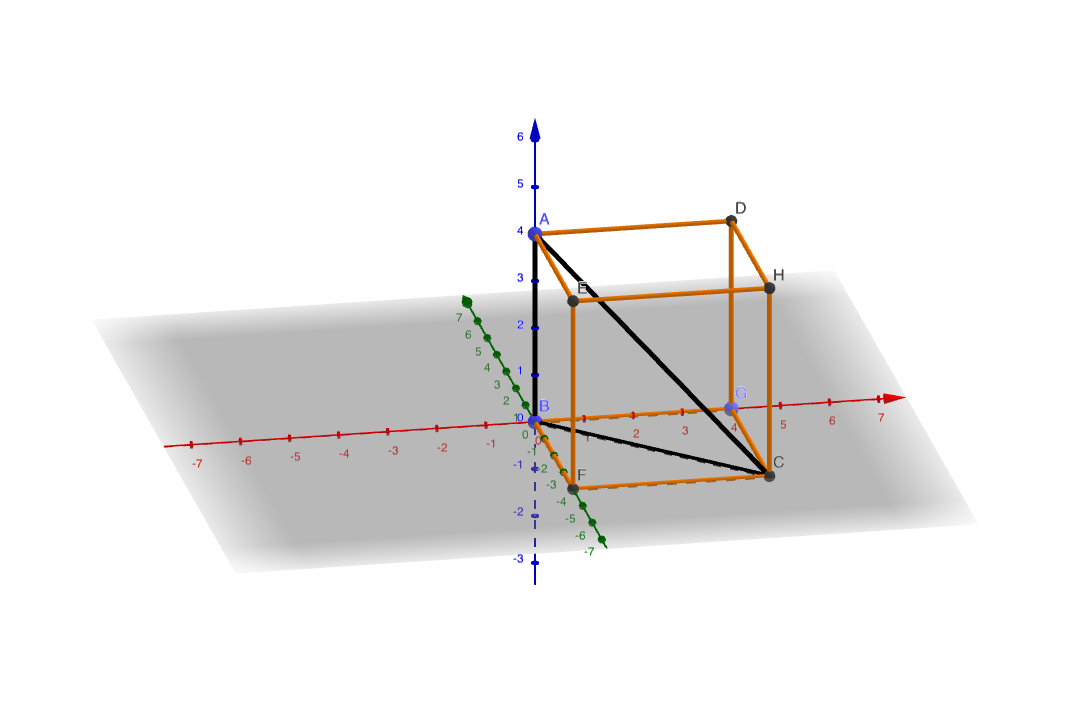
\includegraphics[width=.9\linewidth]{./manip_real/img/cube-sqrt3-png.png}
\caption{Cube d'arrête 1}
\end{figure}
\item Montrons par l'absurde\index{raisonnement!absurde} que \(\sqrt{3}\)
est irrationnel\index{ensembles!des nombres irrationnels}.
Soit \(a\) et \(b\) deux entiers tels que
\[\sqrt{3} = \dfrac{a}{b}\]
et \(pgcd(a, b) = 1\).\index{pgcd}

Alors \(a^2 = 3b^2\).

Puisque \(a\) et \(b\) n'ont pas de diviseur commun il en va de
même pour leurs carrés.

Donc 3 est un diviseur de \(a\) puisqu'il divise son carré.

Ainsi \[a = 3k\] avec \(k\in\mathbb{Z}\).

On peut alors établir que
\[a^2 = 9k^2\]
ce qui implique \[b^2 = 3k^2\]

Comme \(a^2\) et \(b^2\) n'ont pas de diviseur commun (car \(a\) et
\(b\) n'en ont pas) alors \(k^2\) ne divise pas \(b^2\) (car il
divise déjà \(a^2\)).

Mais alors, on a nécessairement 3 comme diviseur de \(b^2\).

Problème, si 3 divise \(b^2\) alors il divise aussi \(b\) ce qui
contredit \(pgcd(a, b) = 1\).\index{pgcd}
\end{enumerate}


\textbf{CQFD}

\begin{itemize}
\item \hyperref[org1486a04]{Voir l'énoncé de l'exercice 11}
page~\pageref{page:sec2.6.5exo11}
\end{itemize}


\clearpage

\section{Solution de l'exercice 12}
\label{sec:org5714eb2}
\label{org86d02ad}
\label{page:sec8.6.3sol12}

\begin{enumerate}
\item Le nombre 4 divise le carré de 10 mais pas 10. Le nombre 8 divise
le carré de 4 mais pas 4. Le nombre 12 divise le carré de 6 mais
pas 6. Le nombre 16 divise le carré de 8 mais pas 8. Le nombre 9
divise le carré de 12 mais pas 12. Le nombre 25 divise le carré de
10 mais pas 10.
\item Supposons par l'absurde que le nombre d'or
\[\Phi = \dfrac{1 + \sqrt{5}}{2}\] soit rationnel.
Alors
\[\Phi = \dfrac{a}{b}\] avec \(pgcd(a, b) = 1\).\index{pgcd}
Or
\[\Phi^2 = 1 + \Phi\]
donc
\[\Phi^2 = \dfrac{a + b}{b}\in\mathbb{Q}\]
mais alors
\[\dfrac{a + b}{b} = \dfrac{a^2}{b^2}\]
conduit à
\[ab + b^2 = a^2\]
soit
\[b^2 = a(a - b)\]
ce qui est absurde car \(a\) ne divise pas \(b\) donc pas son carré
non plus.

\textbf{CQFD}

Pour rappel, si \(a\) divisait \(b\) alors il existerait
\(k\in\mathbb{Z}\) tel que :
\[b = ka\]
Par conséquent on aurait automatiquent :
\[b^2 = (ka)^2 = k^2a^2 = a(ak^2)\]

Formalisons :
\begin{itemize}
\item A = << \(a\) divise \(b\) >>
\item B = << \(a^2\) divise \(b^2\) >>
\item P = << A implique B >> (c'est ce qu'on vient de montrer)
\item P = << si \(a\) divise \(b\) alors \(a^2\) divise \(b^2\) >>
\end{itemize}

Par contraposée :
\begin{itemize}
\item non(A) = << \(a\) ne divise pas \(b\) >>
\item non(B) = << \(a^2\) ne divise pas \(b^2\) >>
\item Q = CP(P) = << non(B) implique non(A) >>
\item Q = CP(P) = << si \(a^2\) ne divise pas \(b^2\) alors \(a\) ne
divise pas \(b\) >>
\end{itemize}

Donc si \(a\) ne divise pas \(b\) il ne peut pas diviser son carré.

\item \hyperref[org677ae69]{Voir l'énoncé de l'exercice 12}
page~\pageref{page:sec2.6.7exo12}
\end{enumerate}


\clearpage

\part{Solutions des exercices des capacités attendues}
\label{sec:orge60ad46}
\label{orgd241bdf}
\label{page:sec9sols-capacities}

\begin{myquote}{John Forbes Nash Jr.}
\enquote{You don’t have to be a mathematician to have a feel for numbers.}
\footnote{Voir la page Wikipédia sur Nash : \url{https://en.wikipedia.org/wiki/John_Forbes_Nash_Jr.}}
\end{myquote}
\index{Nash, John}

\clearpage

\label{orgcabe6f1}
\label{page:sols-capacities-menu}
\begin{itemize}
\item \hyperref[orgfab147a]{Solutions des exercices de la capacité \(C_1\)} page
\pageref{page:sec9.1sols-capacity1}
\item \hyperref[org890787c]{Solutions des exercices de la capacité \(C_2\)} page
\pageref{page:sec9.2sols-capacity2}
\item \hyperref[org0574bca]{Solutions des exercices de la capacité \(C_3\)} page
\pageref{page:sec9.3sols-capacity3}
\item \hyperref[orgaa4998d]{Solutions des exercices de la capacité \(C_4\)} page
\pageref{page:sec9.4sols-capacity4}
\item \hyperref[orge8af971]{Solutions des exercices des contenus} page
\pageref{page:sec8sols-contents}
\end{itemize}



\clearpage

\chapter{Solutions des exercices de la capacité \(C_1\)}
\label{sec:org4901d34}
\label{orgfab147a}
\label{page:sec9.1sols-capacity1}

\begin{myquote}{Sofya Kovalveskaya}
\enquote{It is impossible to be a mathematician without being a poet in soul.}
\footnote{Voir la page Wikipédia sur Kovalveskaya : \url{https://en.wikipedia.org/wiki/Sofya_Kovalevskaya}}
\end{myquote}
\index{Kovalveskaya, Sofya}

\label{orga6feabd}
\label{page:sols-capacity1-menu}
\begin{itemize}
\item \hyperref[orgcc6458f]{Solution de l'exercice 13}
page~\pageref{page:sec9.1.1sols13}
\item \hyperref[orgcabe6f1]{Menu précédent}
page~\pageref{page:sols-capacities-menu}
\end{itemize}

\clearpage

\section{Solution de l'exercice 13}
\label{sec:orge81c56c}
\label{orgcc6458f}
\label{page:sec9.1.1sols13}


Pour rappels tous les codes sont accessibles sur Google Colab à
l'adresse communiquée dans la section concernée lorsque vous
aurez rempli ce petit formulaire : \url{https://forms.gle/qY8ym3ZxSo9NVH3S7}
(vous trouverez également les corrections de tous les exercices du
livre).


\clearpage


\begin{minted}[]{python}
# Solution
import matplotlib.pyplot as plt
import numpy as np

numbers = [
    -2, -0.5, 0,
    1, np.sqrt(2), np.pi
]
labels = [
    'P_0 (-2)', 'P_1 (-0.5)', 'P_2 (0)',
    'P_3 (1)', 'P_4 (sqrt{2})', r'P_5 (\pi)'
]

plt.figure(figsize=(10, 1))

# Ploter une ligne horizontale
plt.plot(
    [min(numbers), max(numbers)],
    [0, 0],
    'k'
)

# Placer les nombres sur la ligne graduée
plt.scatter(
    numbers,
    np.zeros_like(numbers),
    color='red'
)

# Ajouter des étiquettes aux nombres
for i, label in enumerate(labels):
    plt.text(
        numbers[i],
        0.02,
        label,
        ha='center'
    )

# Masquer les axes
plt.axis('off')

plt.show()
\end{minted}

\clearpage

Pour rappels tous les codes sont accessibles sur Google Colab à
l'adresse communiquée dans la section concernée lorsque vous
aurez rempli ce petit formulaire : \url{https://forms.gle/qY8ym3ZxSo9NVH3S7}
(vous trouverez également les corrections de tous les exercices du
livre).


\begin{itemize}
\item \hyperref[org6da0729]{Voir l'énoncé de l'exercice 13}
page~\pageref{page:sec3.2.2exo13}
\end{itemize}


\clearpage
\chapter{Solutions des exercices de la capacité \(C_2\)}
\label{sec:org0e2621a}
\label{org890787c}
\label{page:sec9.2sols-capacity2}

\begin{myquote}{Karl Weierstrass}
\enquote{A mathematician who is not also something of a poet will never be a
complete mathematician.}
\footnote{Lire la page Wikipédia sur Weierstrass : \url{https://en.wikipedia.org/wiki/Karl_Weierstrass}}
\end{myquote}
\index{Weierstrass, Karl}

\clearpage

\label{org882de4a}
\begin{itemize}
\item \hyperref[orgfeec3ba]{Solution de l'exercice 14}
page~\pageref{page:sec9.2.1sol14}
\item \hyperref[orgcabe6f1]{Menu précédent}
page~\pageref{page:sols-capacities-menu}
\end{itemize}

\clearpage
\section{Solution de l'exercice 14}
\label{sec:org5eda210}
\label{orgfeec3ba}
\label{page:sec9.2.1sol14}

Pour rappels tous les codes sont accessibles sur Google Colab à
l'adresse communiquée dans la section concernée lorsque vous
aurez rempli ce petit formulaire : \url{https://forms.gle/qY8ym3ZxSo9NVH3S7}
(vous trouverez également les corrections de tous les exercices du
livre).

C'est également sur Google Colab que vous pourrez tester tous les
programmes qui vous permettent de pratiquer les capacités attendues
de manière interactive.

\clearpage

\begin{minted}[]{python}
# Solution
from math import floor, ceil



def default(number, decimals):
  """
  Cette fonction prend 2 paramètres
  en entrées :
  + number: le nombre qu'on cherche
            à arrondir par défaut
  + decimals: le nombre de chiffres
              après la virgule
  Elle renvoie le nombre arrondi
  par défaut à decimals décimales
  """

  num = floor(number * 10**decimals)
  den = 10**decimals

  return num / den



def excess(number, decimals):
  """
  Cette fonction prend 2 paramètres
  en entrées :
  + number: le nombre qu'on cherche à arrondir
            par excès
  + decimals: le nombre de chiffres
              après la virgule
  Elle renvoie le nombre arrondi
  par excès à decimals décimales
  """

  if number == int(number):
    num = ceil(number * 10**decimals + 1)
  else: num = ceil(number * 10**decimals)
  den = 10**decimals

  return num / den



def get_boundary(nums, method, decimals):
  """
  Cette fonction prend 3 paramètres
  en entrées :
  + nums: nombres dont on cherche la
          borne (inf ou sup)
  + method: la fonction utilisée
            (default ou excess)
  + decimals: le nombre de décimales
  Elle renvoie la liste des bornes
  (que des infs ou que des sups)
  """

  bounds = [
    method(num, decimals) for num in nums
  ]

  return bounds



num_to_square = [1 + i/10 for i in range(5)]
squares = [
  round(n2s**2, 2) for n2s in num_to_square
]
infs = get_boundary(squares, default, 1)
sups = get_boundary(squares, excess, 1)
list_of_intervals = [
  [infs[i], sups[i]] for i in range(len(infs))
]

nums = []
for i in range(len(squares)):
  nums.extend([infs[i], squares[i], sups[i]])
  n2s = num_to_square[i]
  interval = list_of_intervals[i]
  msg = f"{n2s}**2 = {squares[i]} "
  msg += "appartient à l'intervalle "
  msg += f"{interval}"
  print(msg)

plt.figure(figsize=(10, 1))

# Tracer une ligne horizontale
plt.plot(
  [min(nums), max(nums)],
  [0, 0],
  'k'
)

# Placer les nombres sur la ligne graduée
plt.scatter(
  squares, np.zeros_like(squares),
  color='green', marker='x'
)
plt.scatter(
  infs, np.zeros_like(infs),
  color='red', marker='$[$'
)
plt.scatter(
  sups, np.zeros_like(sups),
  color='red', marker='$]$'
)

infs_labels = [str(inf) for inf in infs]
sqrs_labels = [str(sqr) for sqr in squares]
sups_labels = [str(sup) for sup in sups]
# Ajouter des étiquettes aux nombres
for i, inf_label in enumerate(infs_labels):
    plt.text(
      infs[i],
      0.02,
      inf_label,
      ha='center'
    )

for i, sqr_label in enumerate(sqrs_labels):
    plt.text(
      squares[i], -0.02, sqr_label,
      ha='center', va='top'
    )

for i, sup_label in enumerate(sups_labels):
    plt.text(
      sups[i], 0.02,
      sup_label, ha='center'
    )


# Masquer les axes
plt.axis('off')

plt.show()
\end{minted}

\clearpage

Pour rappels tous les codes sont accessibles sur Google Colab à
l'adresse communiquée dans la section concernée lorsque vous
aurez rempli ce petit formulaire : \url{https://forms.gle/qY8ym3ZxSo9NVH3S7}
(vous trouverez également les corrections de tous les exercices du
livre).

C'est également sur Google Colab que vous pourrez tester tous les
programmes qui vous permettent de pratiquer les capacités attendues
de manière interactive.


\begin{itemize}
\item \hyperref[org7d5ffab]{Voir l'énoncé de l'exercice 14}
page~\pageref{page:sec3.3.2exo14}
\end{itemize}

\clearpage
\chapter{Solutions des exercices de la capacité \(C_3\)}
\label{sec:org5469a12}
\label{org0574bca}
\label{page:sec9.3sols-capacity3}

\begin{myquote}{Georg Cantor}
\enquote{In mathematics the art of proposing a question must be held of
higher value than solving it.}
\footnote{Voir la page Wikipédia sur Cantor : \url{https://en.wikipedia.org/wiki/Georg_Cantor}}
\end{myquote}
\index{Cantor, Georg}

\clearpage

\label{org58d9008}
\label{page:sols-capacity3-menu}
\begin{itemize}
\item \hyperref[orgb7308e1]{Solution de l'exercice 15}
page~\pageref{page:sec9.3.1-sol15}
\item \hyperref[org2f710b4]{Solution de l'exercice 16}
page~\pageref{page:sec9.3.2sol16}
\item \hyperref[orgcabe6f1]{Menu précédent}
page~\pageref{page:sols-capacities-menu}
\end{itemize}

\clearpage

\section{Solution de l'exercice 15}
\label{sec:org6009dd6}
\label{orgb7308e1}
\label{page:sec9.3.1-sol15}

Les solutions sont générées automatiquement après la saisie
utilisateur.

Pour rappels tous les codes sont accessibles sur Google Colab à
l'adresse communiquée dans la section concernée lorsque vous
aurez rempli ce petit formulaire : \url{https://forms.gle/qY8ym3ZxSo9NVH3S7}
(vous trouverez également les corrections de tous les exercices du
livre).

C'est également sur Google Colab que vous pourrez tester tous les
programmes qui vous permettent de pratiquer les capacités attendues
de manière interactive.

\begin{itemize}
\item \hyperref[org8cc10b8]{Voir l'énoncé de l'exercice 15}
page~\pageref{page:sec3.4.1exo15}
\end{itemize}



\clearpage

\section{Solution de l'exercice 16}
\label{sec:orgefbe07e}

\label{org2f710b4}
\label{page:sec9.3.2sol16}

Les solutions sont générées automatiquement après la saisie
utilisateur.

Pour rappels tous les codes sont accessibles sur Google Colab à
l'adresse communiquée dans la section concernée lorsque vous
aurez rempli ce petit formulaire : \url{https://forms.gle/qY8ym3ZxSo9NVH3S7}
(vous trouverez également les corrections de tous les exercices du
livre).

C'est également sur Google Colab que vous pourrez tester tous les
programmes qui vous permettent de pratiquer les capacités attendues
de manière interactive.


\begin{itemize}
\item \hyperref[org70c1962]{Voir l'énoncé de l'exercice 16}
page~\pageref{page:sec3.4.2exo16}
\end{itemize}

\clearpage

\chapter{Solutions des exercices de la capacité \(C_4\)}
\label{sec:org9bd0fb3}
\label{orgaa4998d}
\label{page:sec9.4sols-capacity4}

\begin{myquote}{John Wesley Young}
\enquote{It is clear that the chief end of mathematical study must be to
make the students think.}
\footnote{Lire la page Wikipédia sur Young : \url{https://en.wikipedia.org/wiki/John_Wesley_Young}}
\end{myquote}
\index{Young, John}

\clearpage

\label{org8c5c90a}
\label{page:sols-capacity4-menu}
\begin{itemize}
\item \hyperref[orgef40258]{Solution de l'exercice 17}
page~\pageref{page:sec9.4.1sol17}
\item \hyperref[orgcabe6f1]{Menu précédent}
page~\pageref{page:sols-capacities-menu}
\end{itemize}

\clearpage
\section{Solution de l'exercice 17}
\label{sec:orga5f9661}
\label{orgef40258}
\label{page:sec9.4.1sol17}

Pour rappels tous les codes sont accessibles sur Google Colab à
l'adresse communiquée dans la section concernée lorsque vous
aurez rempli ce petit formulaire : \url{https://forms.gle/qY8ym3ZxSo9NVH3S7}
(vous trouverez également les corrections de tous les exercices du
livre).

C'est également sur Google Colab que vous pourrez tester tous les
programmes qui vous permettent de pratiquer les capacités attendues
de manière interactive.

\begin{itemize}
\item \hyperref[org4f79895]{Voir l'énoncé de l'exercice 17}
page~\pageref{page:sec3.5.1exo17}
\end{itemize}

\part{Remerciements}
\label{sec:orgc32fb54}

Merci d’avoir lu ce livre jusqu’au bout.

Si tu as aimé cette exploration des nombres réels, je t’invite à :
\begin{itemize}
\item Laisser un avis sur Amazon
\item Mettre le maximum d'étoiles sur Amazon
\item Partager le livre autour de toi
\item Me contacter pour des suggestions
\end{itemize}

\begin{center}
\includegraphics[width=1.5in]{./manip_real/img/qr-code.png}
\end{center}

Scanne ce QR code pour accéder directement à la page du livre sur Amazon.
\part{Index}
\label{sec:org01bac78}
\printindex


\printglossaries
\printglossary[type=\acronymtype]
\end{document}
